\subsection{Outline}
In this section, all the main results for 5.02 TeV Pb+Pb are presented as follows:
\begin{itemize}
\item Comparison between standard and 3-subevent cumulant;
\item 2-particle cumulant $c_n\{2\}$;
\item 4-particle cumulant $c_n\{4\}$ and $nc_n\{4\}$;
\item 4-particle cumulant in ultra-central collisions;
\item 4-particle cumulant in 2.76 and 5.02 TeV;
\item 6-particle cumulant $c_n\{6\}$ and $nc_n\{6\}$;
\item Universality check of flow fluctuation models;
\item Symmetric cumulant $sc_{n,m}\{4\}$ and $nsc_{n,m}\{4\}$;
\item Asymmetric cumulant $ac_{n,n+m}\{3\}$ and $nac_{n,n+m}\{3\}$;
\end{itemize}
Most of the results are calculated using standard cumulant method, and they are presented in the following 4 $p_\text{T}$ ranges:
\begin{itemize}
\item $0.5<p_\text{T}<5.0$ GeV
\item $1.0<p_\text{T}<5.0$ GeV
\item $1.5<p_\text{T}<5.0$ GeV
\item $2.0<p_\text{T}<5.0$ GeV
\end{itemize}
In additional, three different event class definitions are applied to test impact of centrality on flow fluctuations:
\begin{itemize}
\item Event class definition 1: centrality: defined by FCal $E_\text{T}$;
\item Event class definition 2: FCal $E_\text{T}$: same as centrality but with better look in UCC;
\item Event class definition 3: $N_{ch}^{rec}$: different $\eta$ range from FCal $E_\text{T}$;
\end{itemize}

\subsection{Comparison between standard and 3-subevent cumulant}
3-subevent method was proposed to suppress the residual non-flow contribution. It measures particle correlation across different $\eta$ ranges. The method has been extensively studied in small systems and proven its effectiveness. However, in large systems like Pb+Pb collision, where flow signal is dominating over non-flow, the improvement from 3-subevent method is limited. In this section, we will make direct comparison between results using standard and 3-subevent methods. If the difference is not large, standard method will be the default method due to its smaller statistical uncertainties.

\begin{figure}[H]
\centering
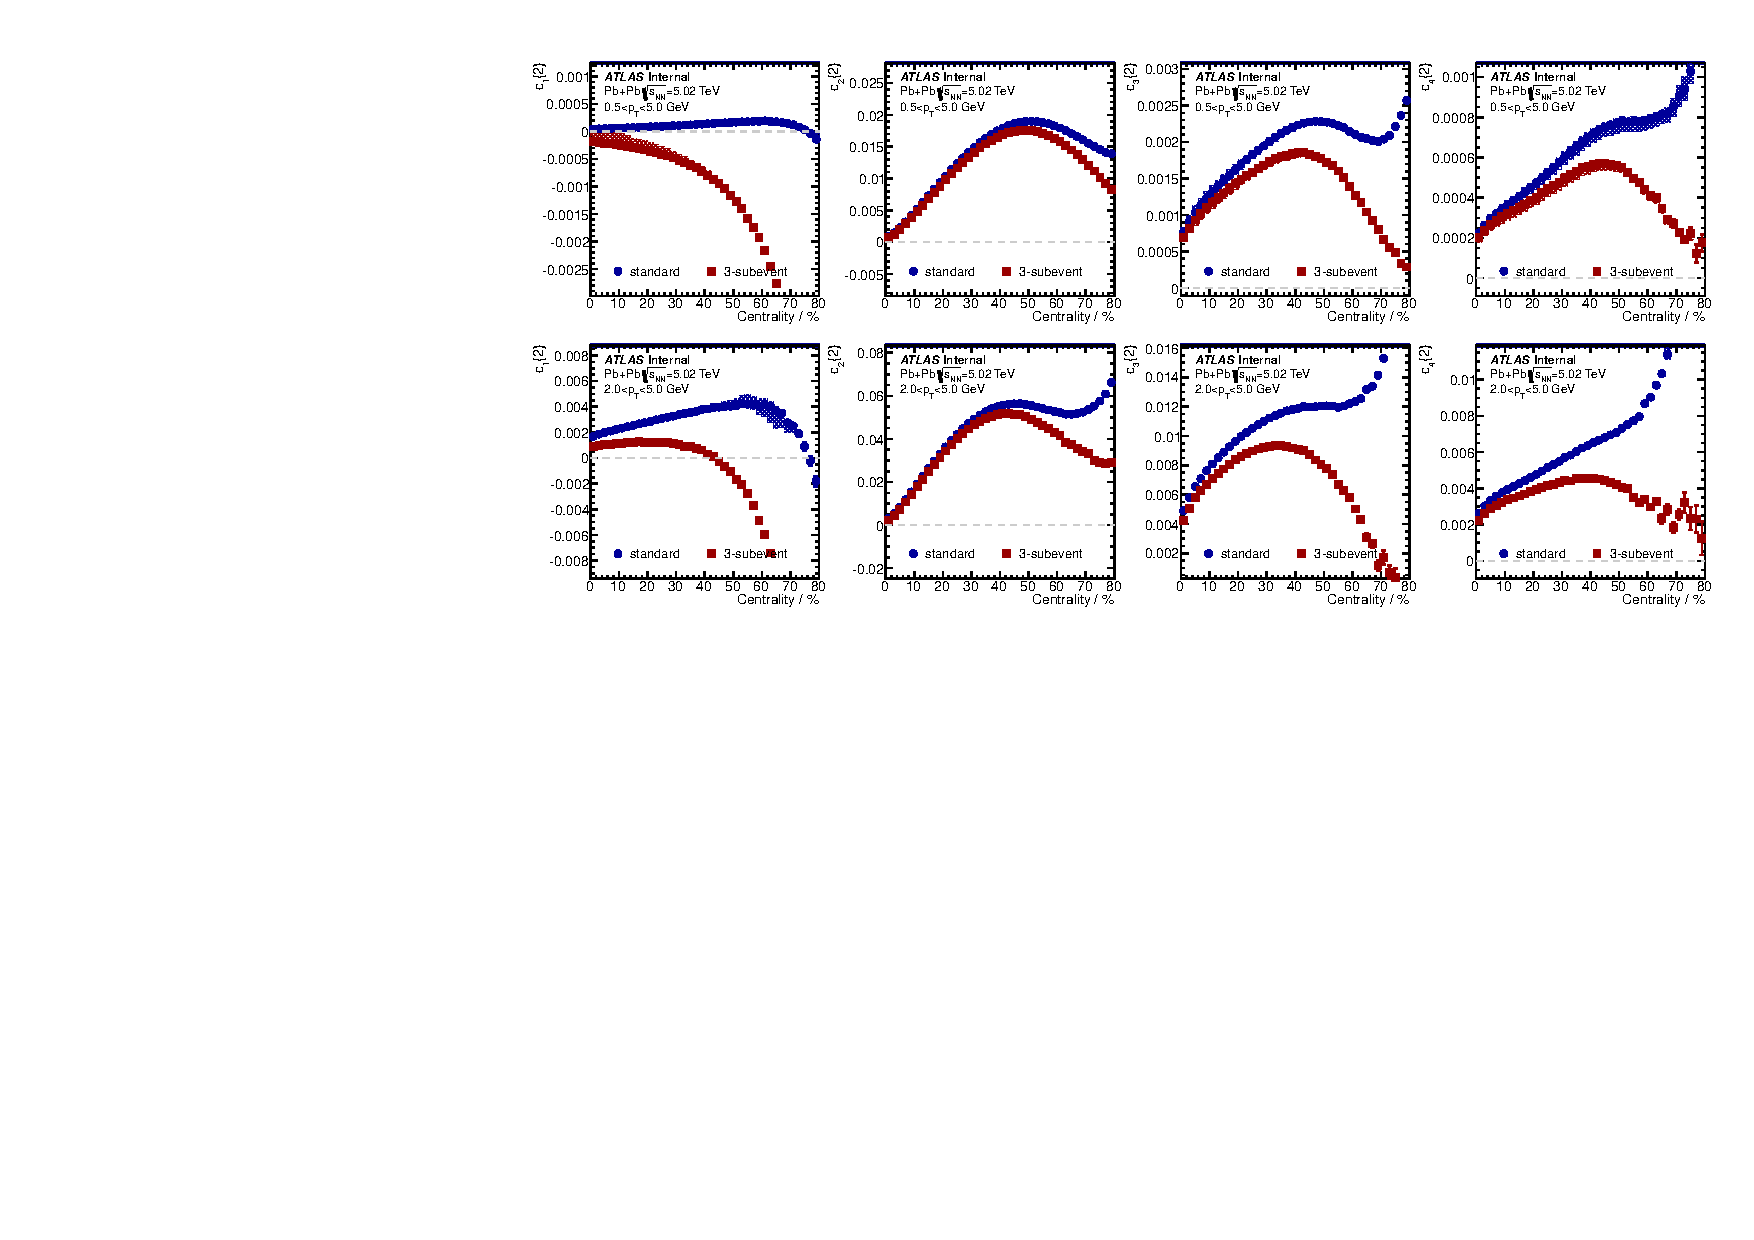
\includegraphics[width=.95\linewidth]{figs/sec_result/forQM/mtd_c2.pdf}
\caption{$c_n\{2\}$ compared between standard and 3-subevent methods, with low $p_\text{T}$ (top) and high $p_\text{T}$ (bottom). Different columns are for different harmonics.}
\label{fig:result_mtd_c2}
\end{figure}
Fig.~\ref{fig:result_mtd_c2} compares the 2-particle cumulant $c_n\{2\}$ using two methods. For second-harmonic $v_2$, the differences between two methods are small in central and mid-central collisions. As the collision moves to peripheral, since number of particles deceases fast, the non-flow contributions case the growth of the differences between two methods. While for other flow harmonics, due to their smaller magnitudes, the suppression from 3-subevent method is observed even in central collision. The huge differences in $v_1$ is partially due to the large momentum conservation effects in standard method, which we will not discuss in details in this analysis ($c_1\{2\}$ is not included in the results). Since the statistical uncertainty for 2-particle correlation is not an issue, in order to suppress the non-flow, in this analysis, 3-subevent method is always preferred whenever 2-particle correlations are calculated (for example in the normalized cumulant).

\begin{figure}[H]
\centering
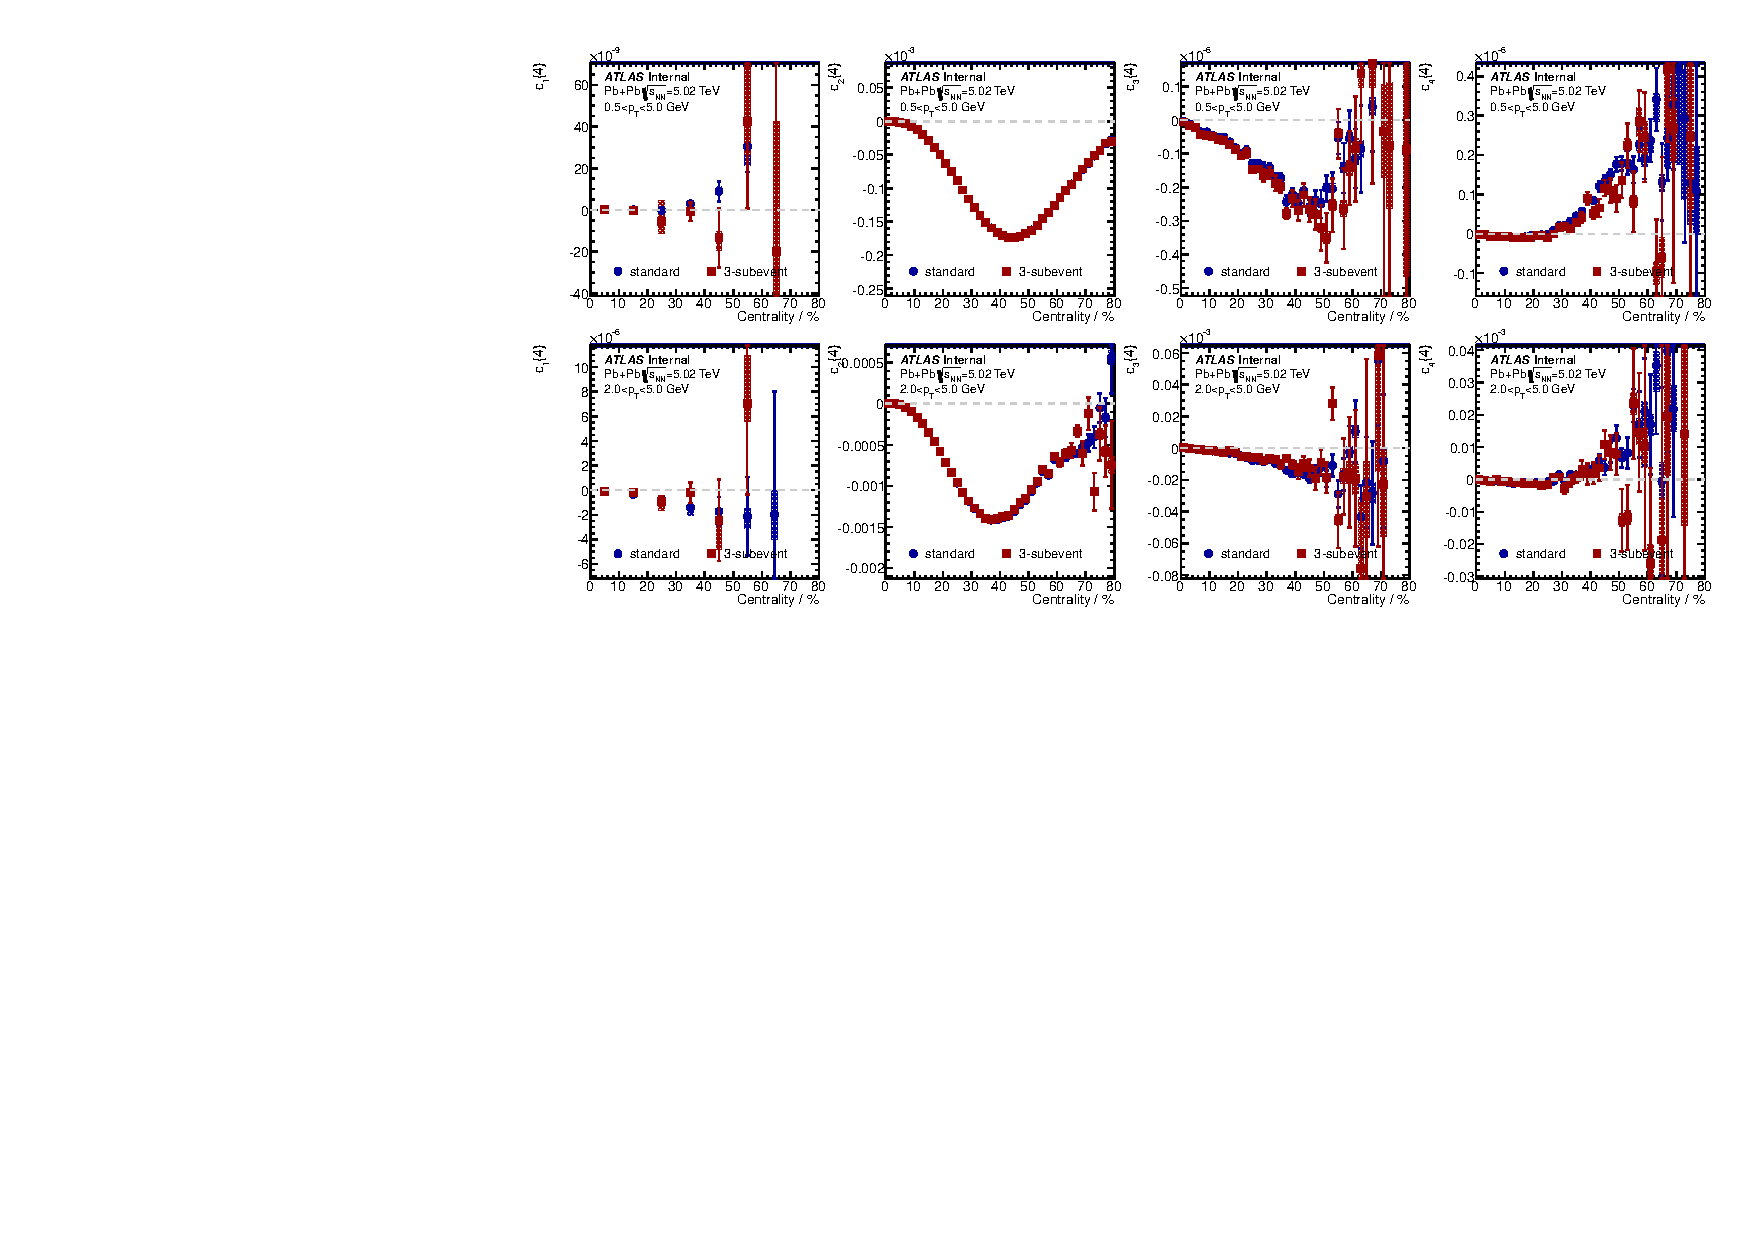
\includegraphics[width=.95\linewidth]{figs/sec_result/forQM/mtd_c4.pdf}
\caption{$c_n\{4\}$ compared between standard and 3-subevent methods, with low $p_\text{T}$ (top) and high $p_\text{T}$ (bottom). Different columns are for different harmonics.}
\label{fig:result_mtd_c4}
\end{figure}
Fig.~\ref{fig:result_mtd_c4} compares the 4-particle cumulant $c_n\{4\}$ using standard and 3-subevent methods. For $v_2$, both methods give very consistent $c_2\{4\}$. This is as expected since by requiring 4 particles in the correlation calculation, the non-flow contributions are already significantly suppressed. For $v_3$ and $v_4$, both methods are consistent within statistical uncertainties, and we do see the errors from 3-subevent are much larger. For $v_1$ in high $p_\text{T}$, 3-subevent method can also measure negative $c_1\{4\}$ in peripheral region, but with smaller statistical significance. This observation supports our claim that negative $c_1\{4\}$ is not due to non-flow contributions.

\begin{figure}[H]
\centering
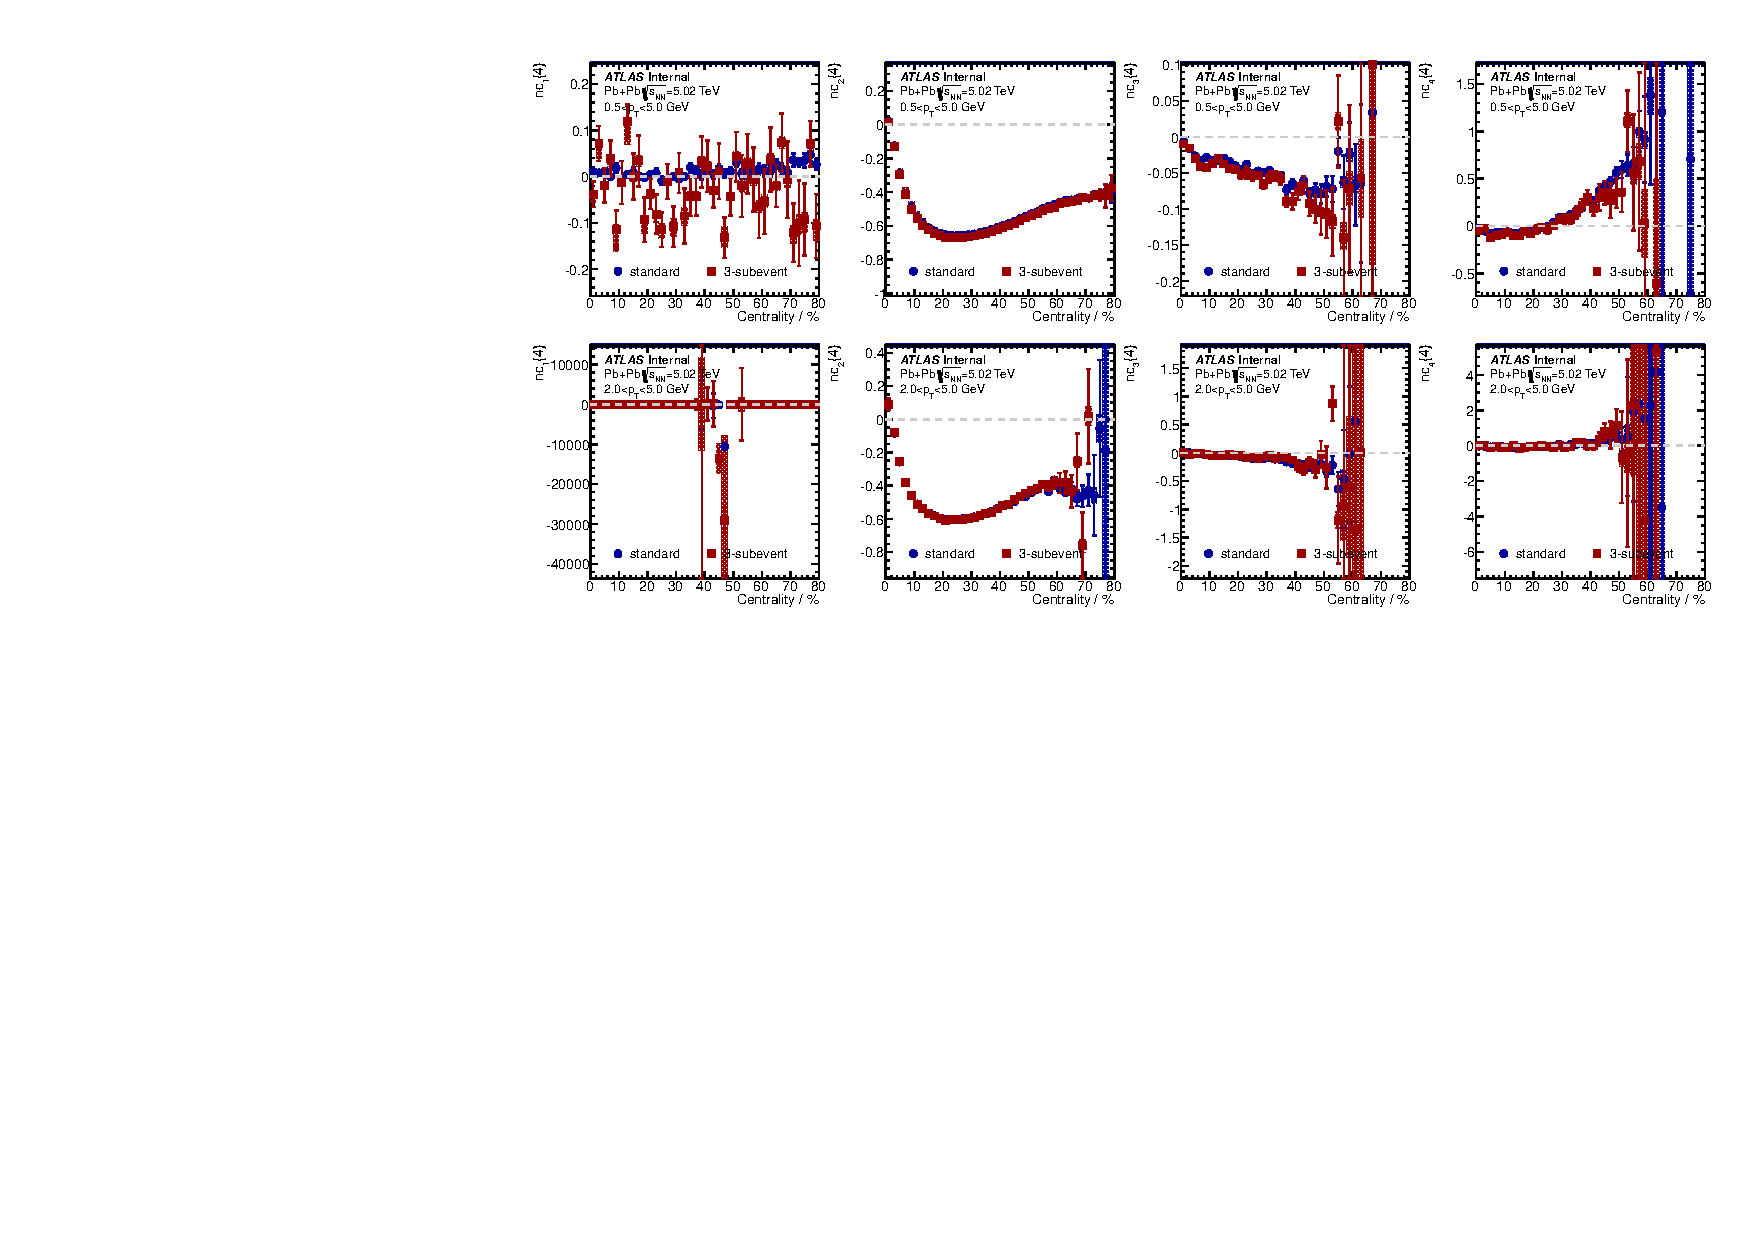
\includegraphics[width=.95\linewidth]{figs/sec_result/forQM/mtd_nc4.pdf}
\caption{$nc_n\{4\}$ compared between standard and 3-subevent methods, with low $p_\text{T}$ (top) and high $p_\text{T}$ (bottom). Different columns are for different harmonics.}
\label{fig:result_mtd_nc4}
\end{figure}
Fig.~\ref{fig:result_mtd_nc4} shows the results for normalized 4-particle cumulant. Since both standard and 3-subevent cumulants are normalized by the 3-subevent 2-particle correlation, the behaviors of $nc_n\{4\}$ are the same as $c_n\{4\}$: both methods give consistent results. (Please ignore the leftmost column because $c_1\{2\}$ is not well defined.)

\begin{figure}[H]
\centering
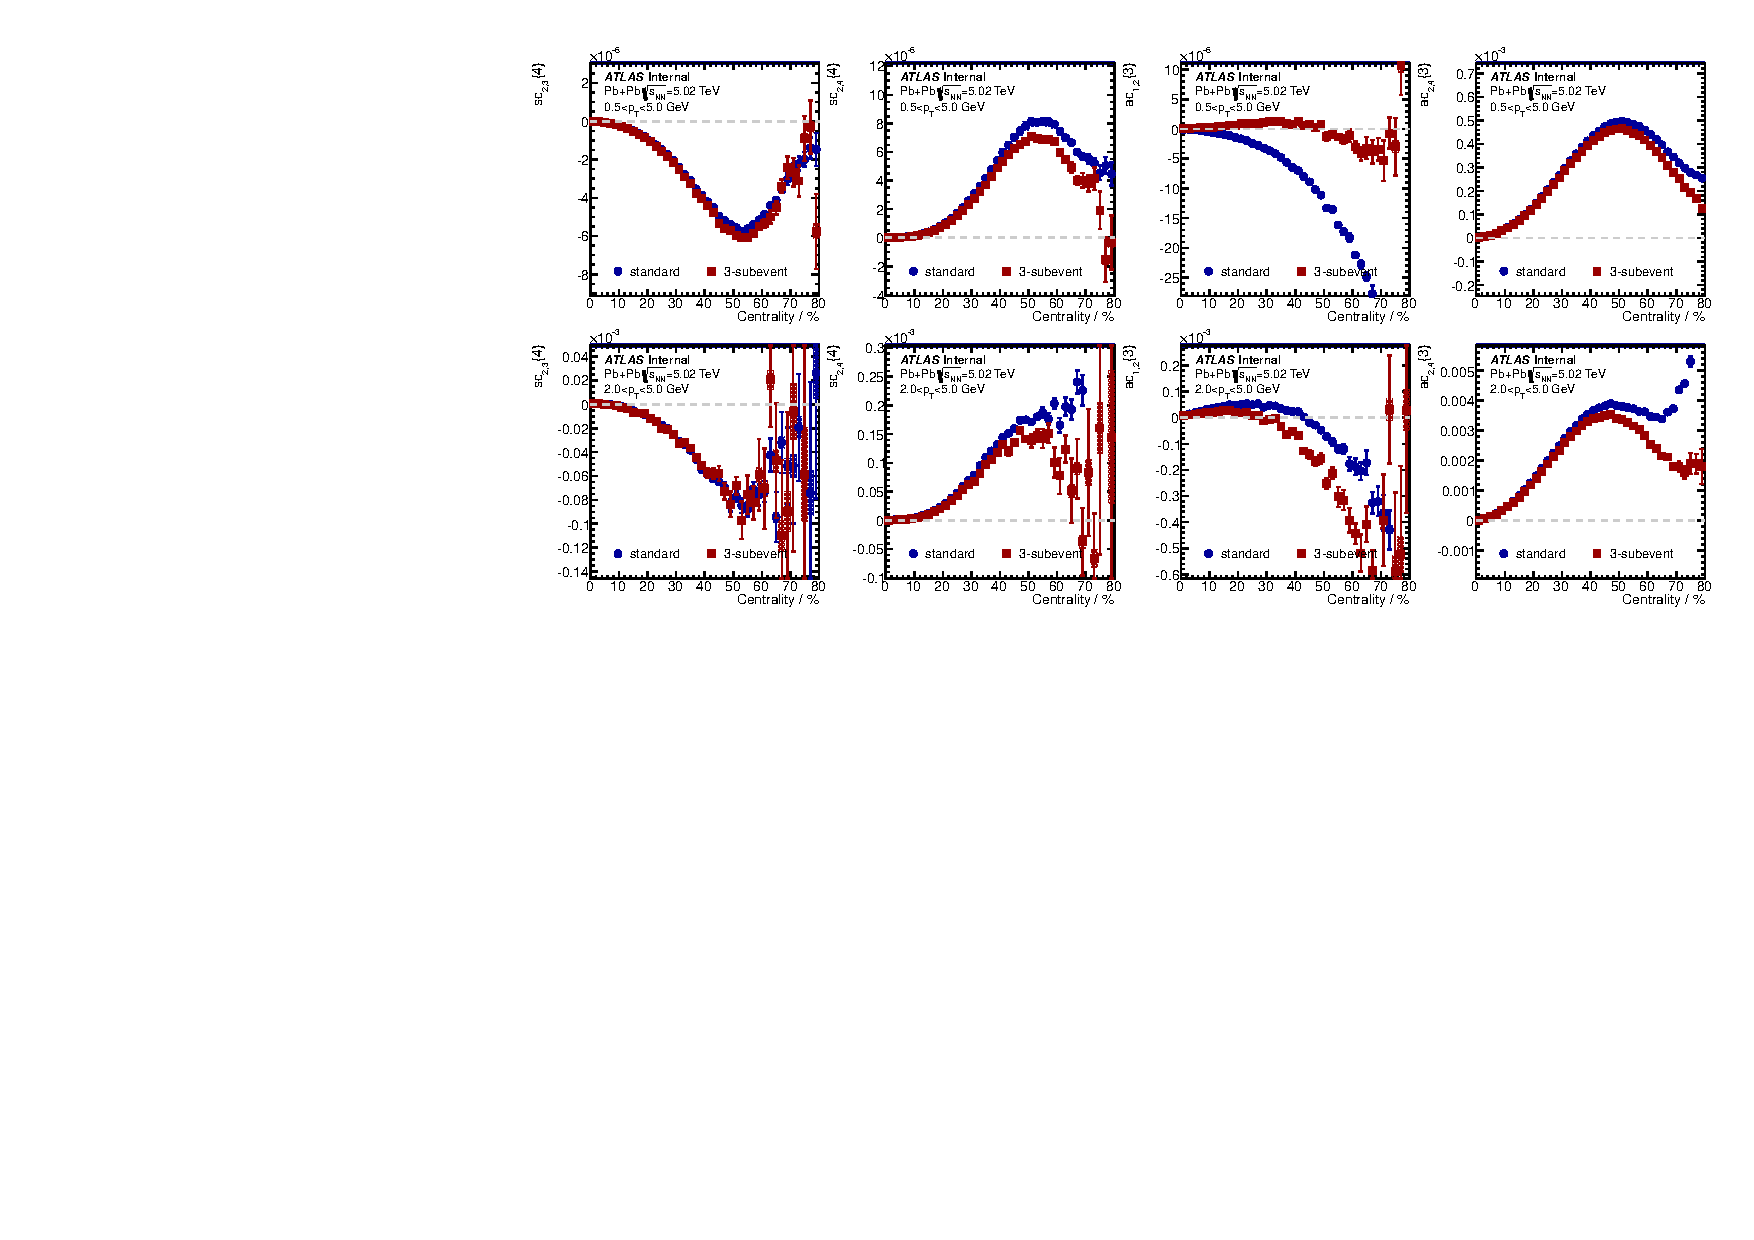
\includegraphics[width=.95\linewidth]{figs/sec_result/forQM/mtd_sc.pdf}
\caption{Symmetric and asymmetric cumulant compared between standard and 3-subevent methods, with low $p_\text{T}$ (top) and high $p_\text{T}$ (bottom). Different columns are for different observables.}
\label{fig:result_mtd_sc}
\end{figure}
In the end, Fig.~\ref{fig:result_mtd_sc} compares the 2 methods for symmetric and asymmetric cumulants. For the observables shown in the figure, both methods began to deviate towards peripheral collisions. The differences can be caused by two factors: non-flow contributions and flow decorrelation effects. Flow decorrelation effects are introduced into 3-subevent method simply because 3 events are separated in the $\eta$ direction. Since in this analysis we do not tend to discuss such effects, the standard method is selected as the default one when presenting the symmetric and asymmetric cumulant results.

\subsection{2-particle cumulant $c_n\{2\}$}
In this section we will show the 2-particle cumulant $c_n\{2\}$ for flow harmonics $v_2$, $v_3$ and $v_4$. In each case, the $c_n\{2\}$ is calculated with 4 different $p_\text{T}$ ranges and 3 different event class definitions. By varying the event class definitions, flow fluctuation is changing in each event class according so that we could study the potential impact of event class definition on cumulant-like analysis.

The main purpose of calculating 2-particle cumulant is to normalize 4-, 6-particle cumulant, symmetric and asymmetric cumulants. In order to suppress the large residual non-flow, we will always apply the 3-subevent method when calculate 2-particle correlation.
\begin{figure}[H]
\centering
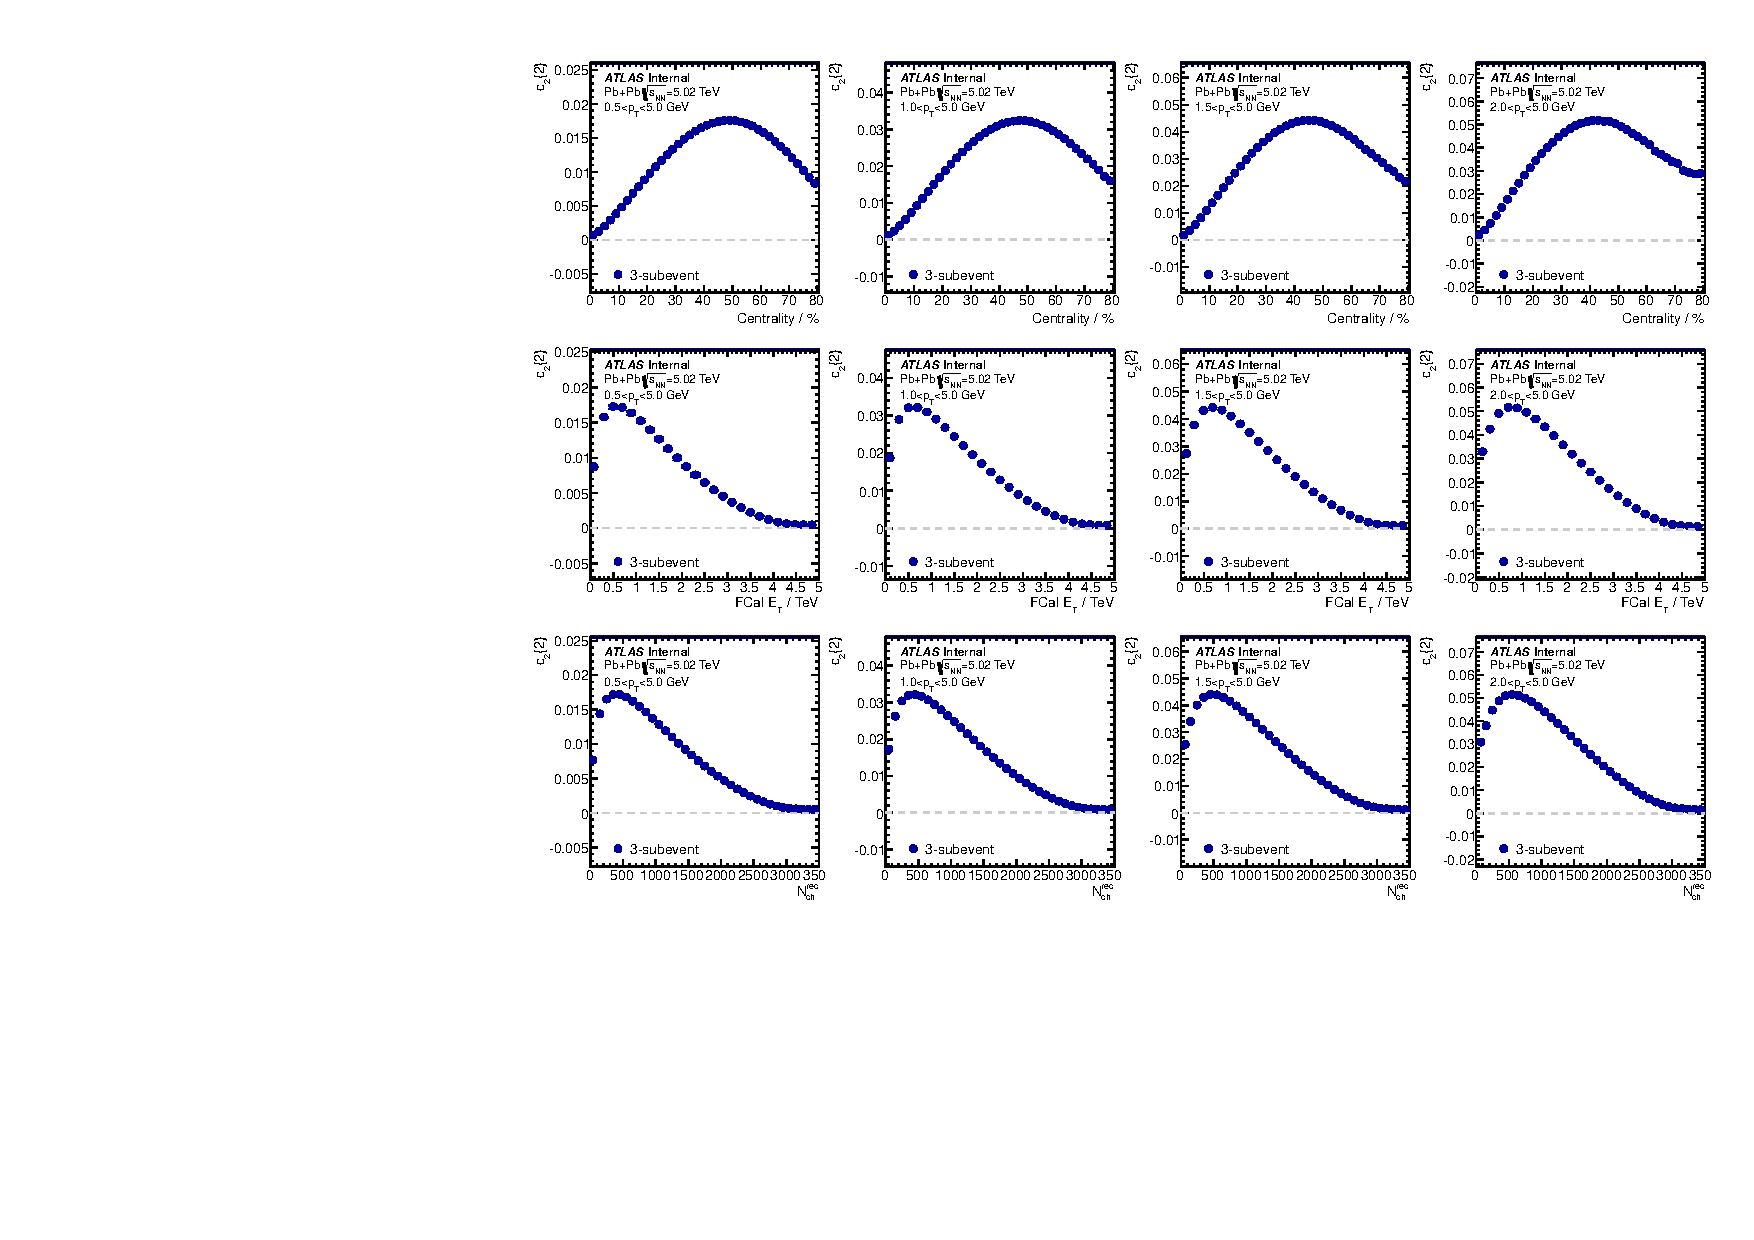
\includegraphics[width=.95\linewidth]{figs/sec_result/forQM/phy_c2_Har2.pdf}
\caption{2-particle cumulant $c_2\{2\}$ calculated with different $p_\text{T}$ ranges (columns) and different event class definitions (rows).}
\label{fig:result_phy_c2_Har2}
\end{figure}
Fig.~\ref{fig:result_phy_c2_Har2} shows the 2-particle cumulant $c_2\{2\}$ calculated with different $p_\text{T}$ ranges and different event class definitions. The centrality dependence of $v_2$ is same as other event-plane measurements: $c_2\{2\}$ is largest in mid-central and decreases towards central and peripheral. Previous measurements showed that $v_2$ as a function of $p_\text{T}$ keeps increasing until $p_\text{T}$ reaches 2 to 3 GeV, which is also reflected in this measurement of $c_2\{2\}$ with different $p_\text{T}$ cuts: the magnitude of $c_2\{2\}$ keeps increasing as $p_\text{T}$ grows. Similar behaviors are observed for other harmonics $v_3$ and $v_4$, as shown in Fig.~\ref{fig:result_phy_c2_Har34}.

\begin{figure}[H]
\centering
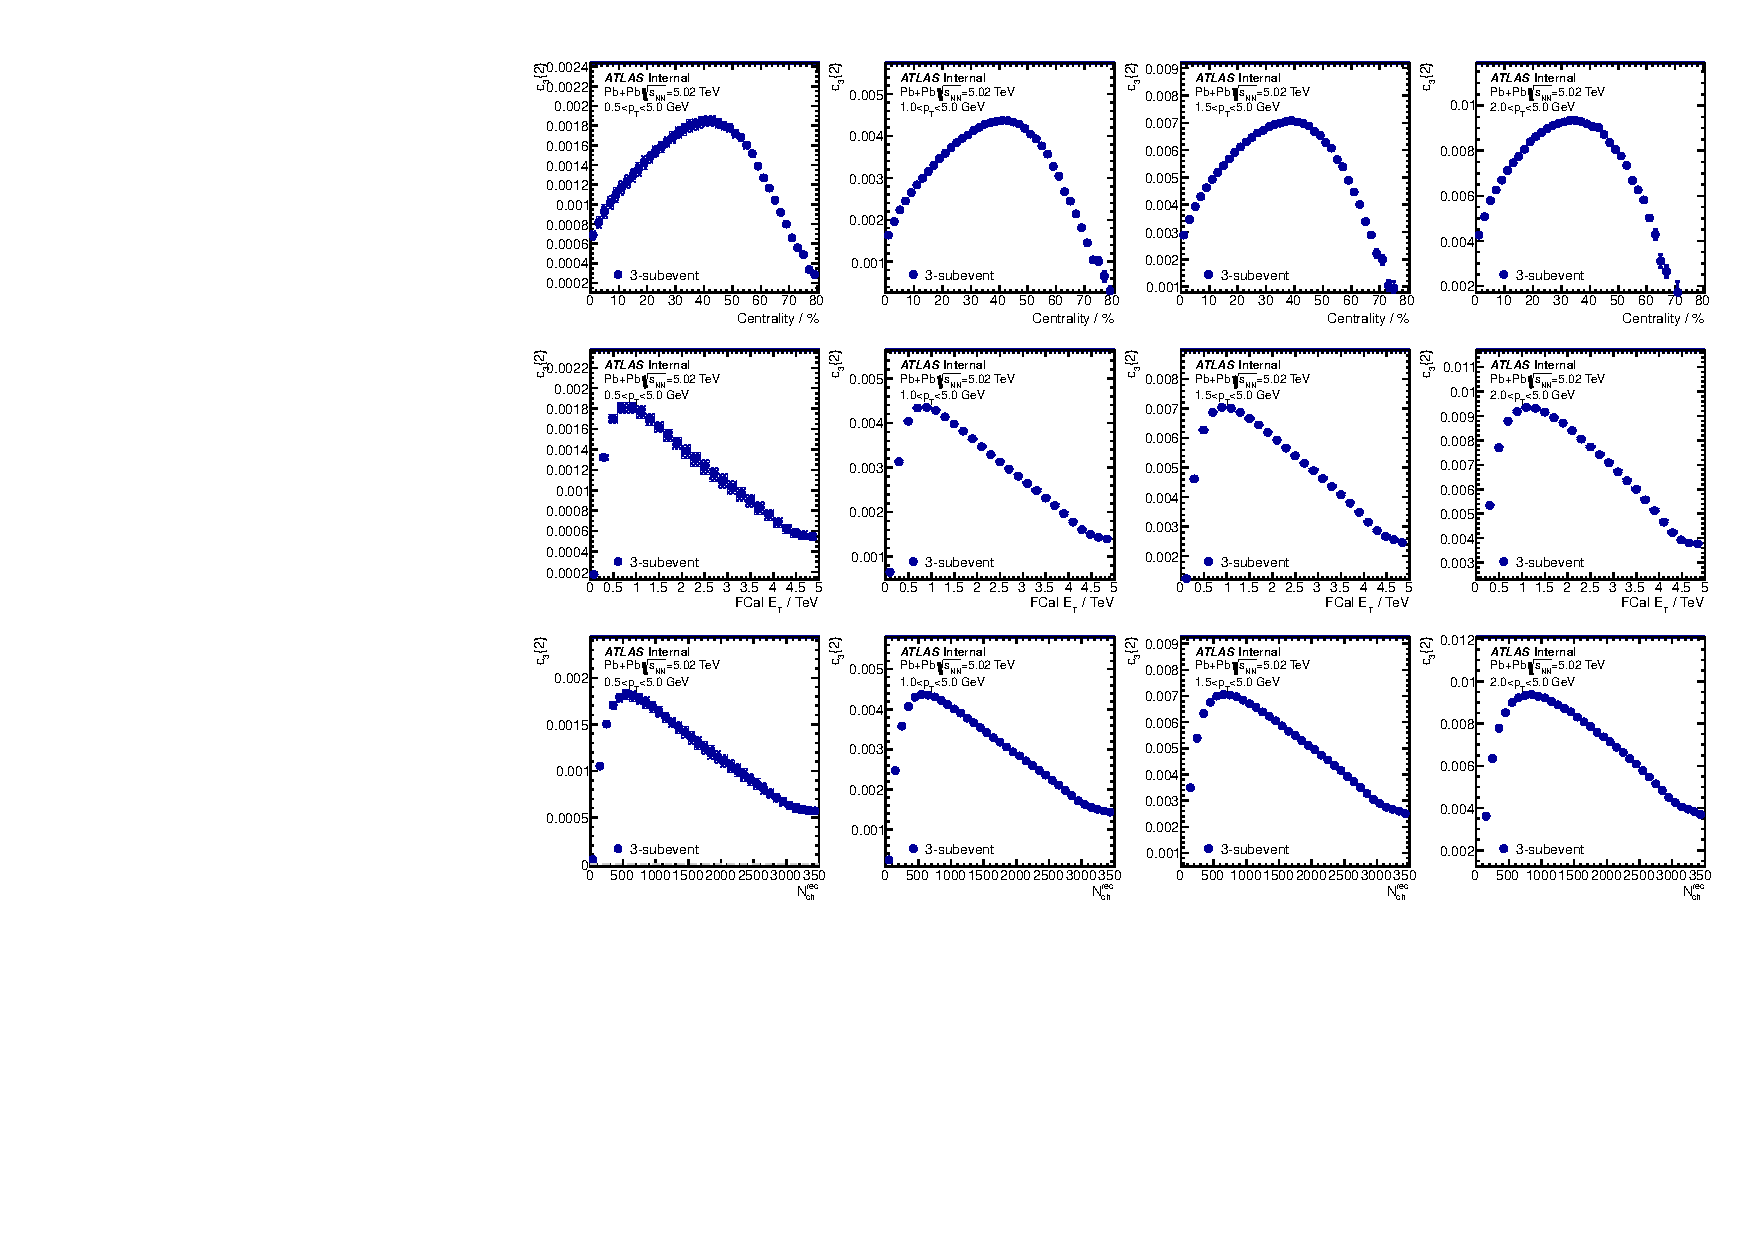
\includegraphics[width=.95\linewidth]{figs/sec_result/forQM/phy_c2_Har3.pdf}
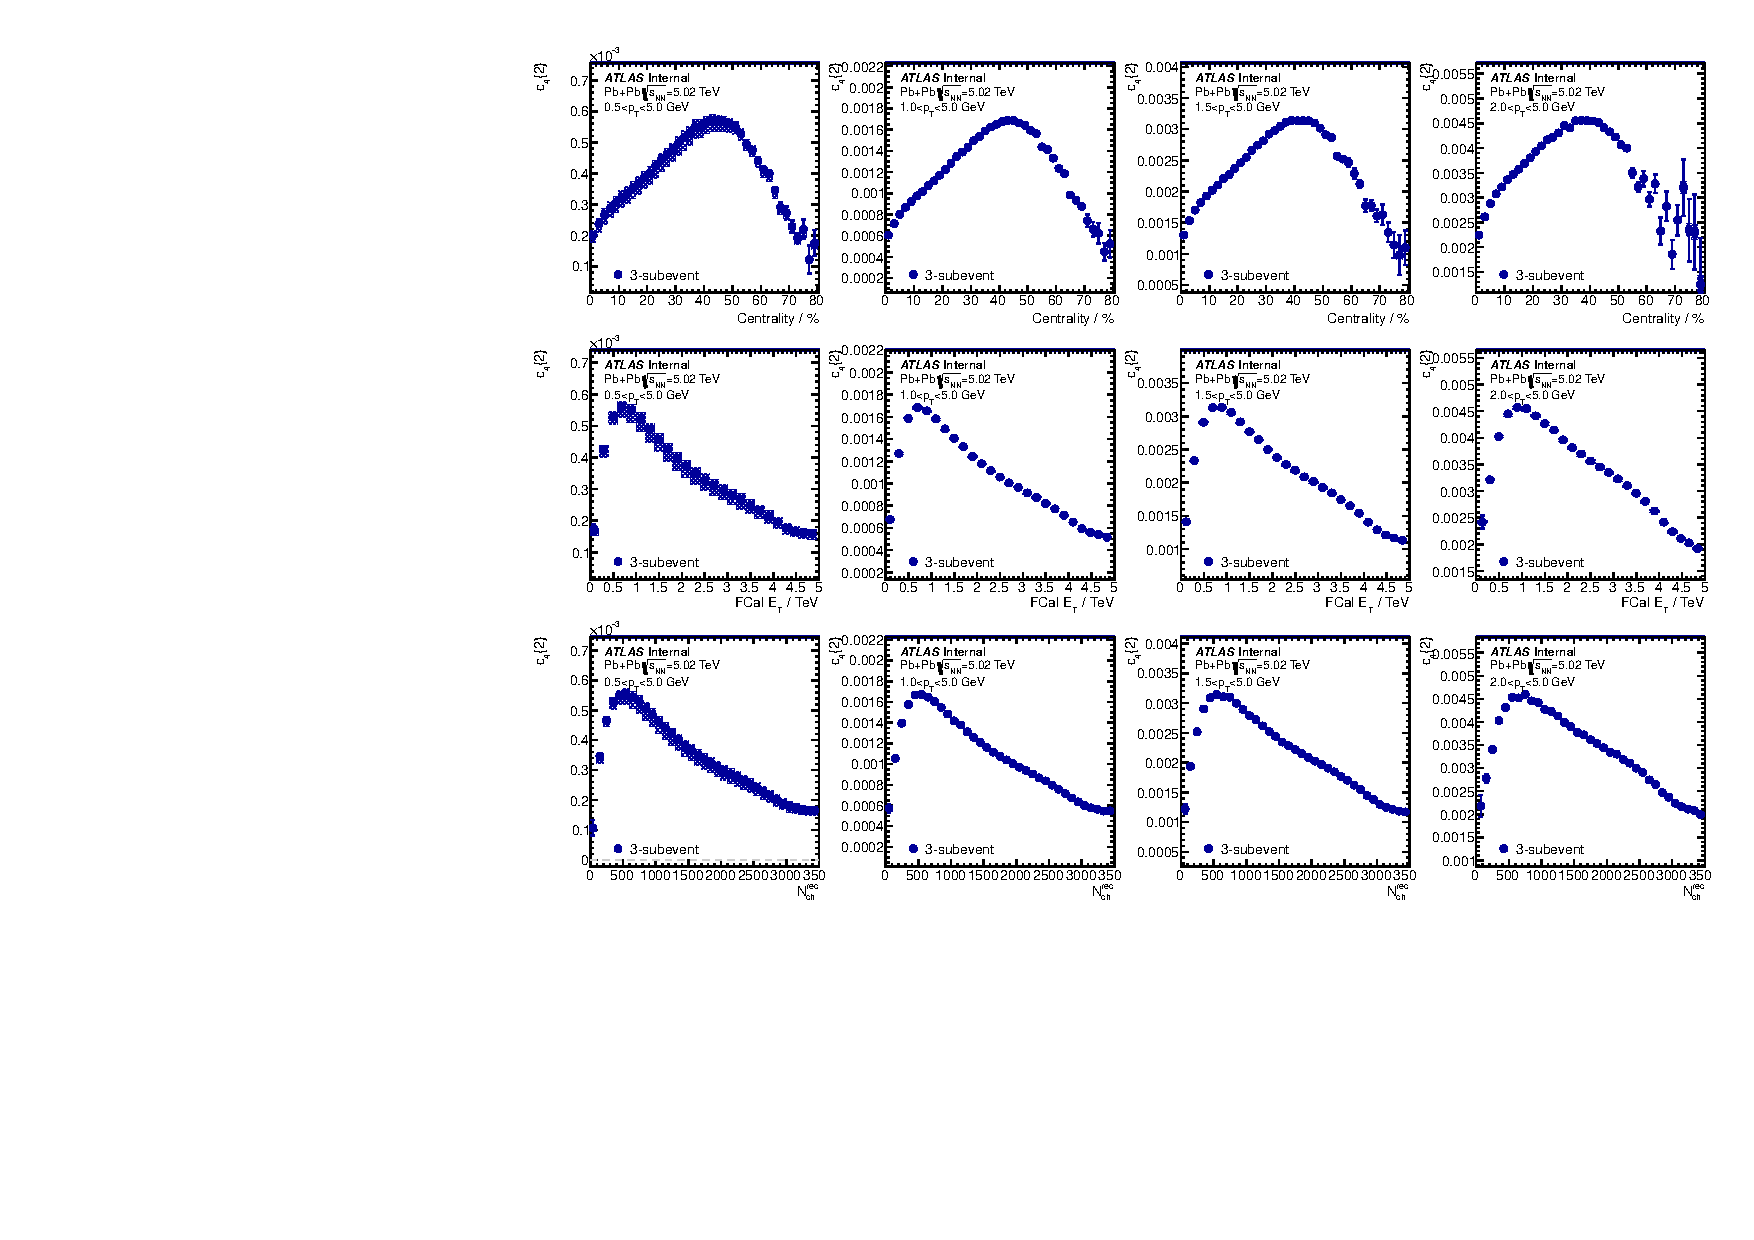
\includegraphics[width=.95\linewidth]{figs/sec_result/forQM/phy_c2_Har4.pdf}
\caption{2-particle cumulant $c_3\{2\}$ (top half) and $c_4\{2\}$ (bottom half) calculated with different $p_\text{T}$ ranges (columns) and different event class definitions (rows).}
\label{fig:result_phy_c2_Har34}
\end{figure}

\subsection{4-particle cumulant $c_n\{4\}$ and $nc_n\{4\}$}
In this section we present the 4-particle cumulant $c_n\{4\}$ for flow harmonics $v_1$, $v_2$, $v_3$ and $v_4$. The normalized cumulants are also shown to better reflect the centrality dependence of flow fluctuations.
\begin{figure}[H]
\centering
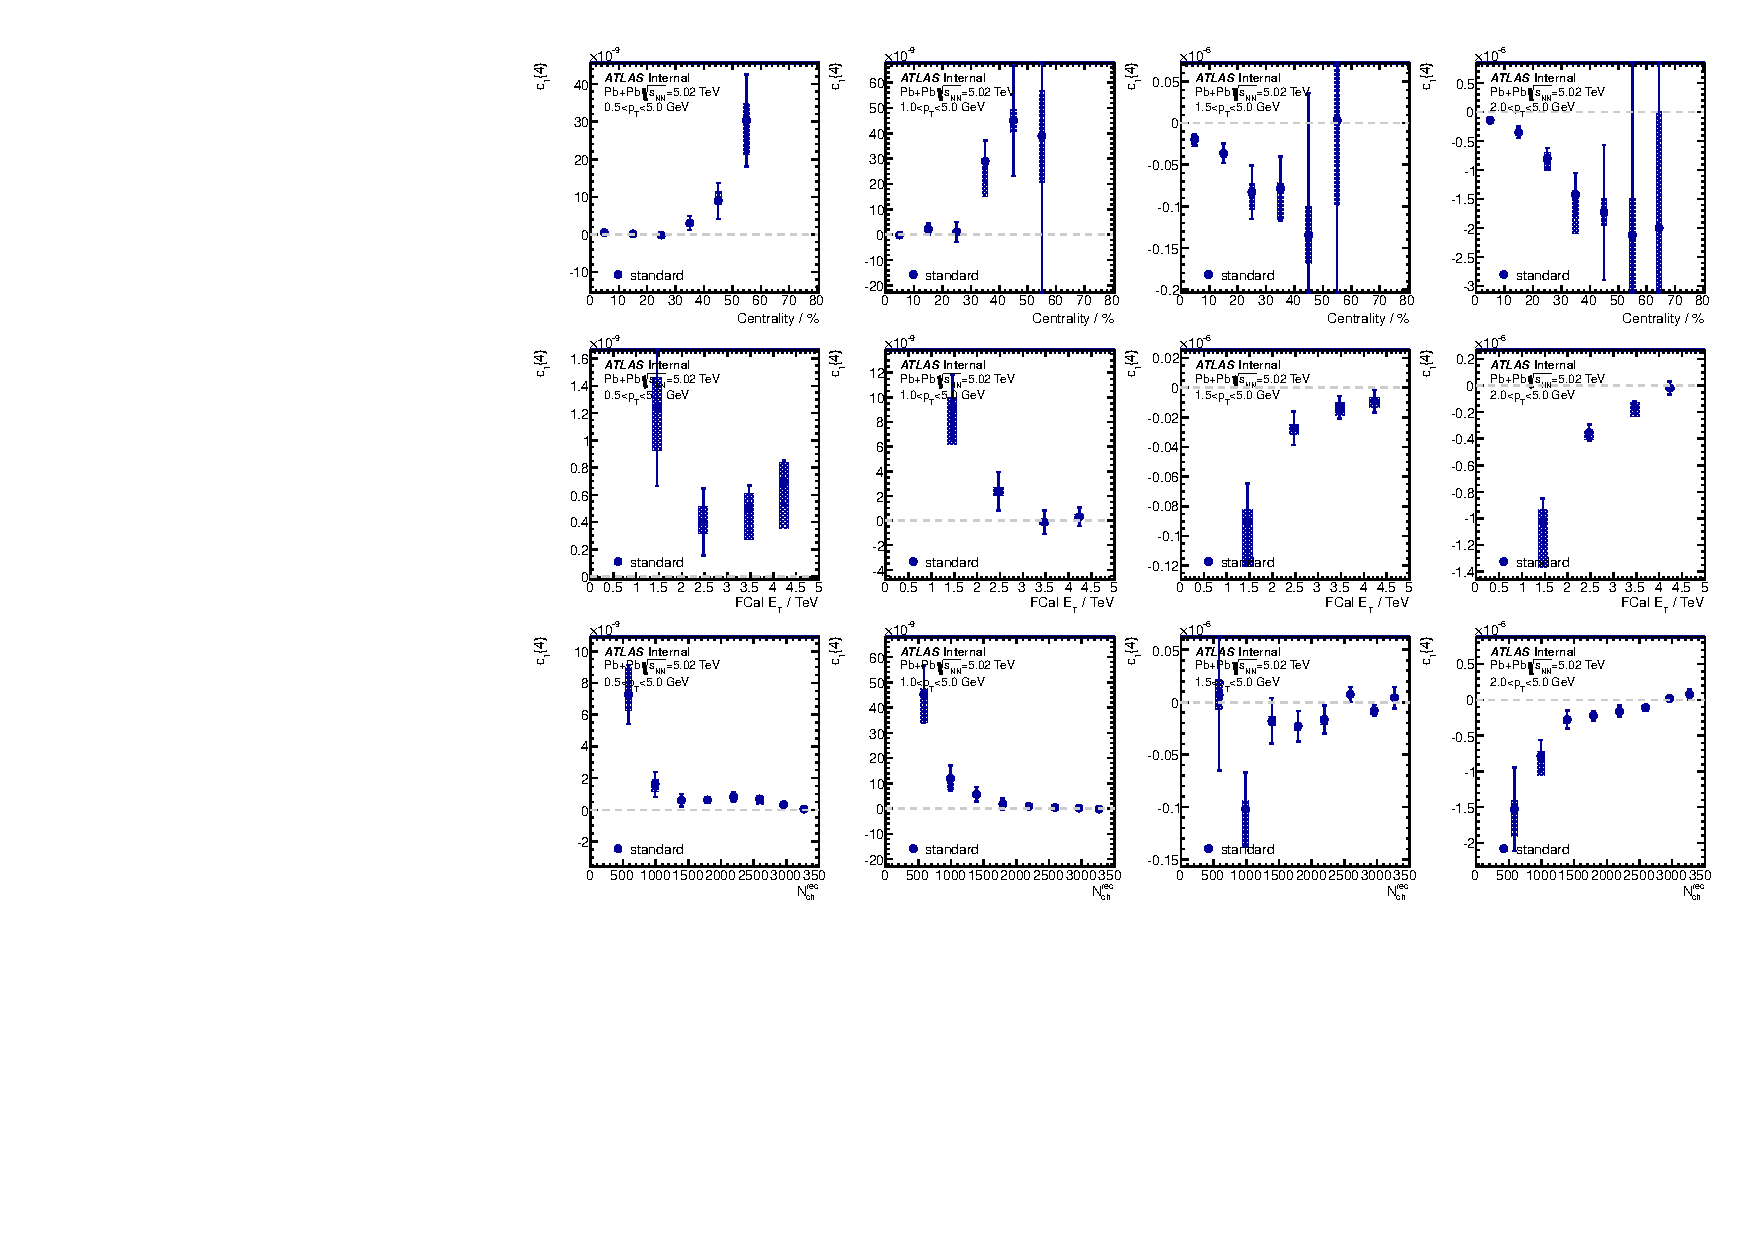
\includegraphics[width=.95\linewidth]{figs/sec_result/forQM/phy_c4_Har1.pdf}
\caption{4-particle cumulant $c_1\{4\}$ calculated with different $p_\text{T}$ ranges (columns) and different event class definitions (rows).}
\label{fig:result_phy_c4_Har1}
\end{figure}
Fig.~\ref{fig:result_phy_c4_Har1} shows the 4-particle cumulant $c_1\{4\}$ calculated with different $p_\text{T}$ ranges and different event class definitions. When the minimum $p_\text{T}$ cut is below 1.0 GeV, $c_1\{4\}$ is consistent with 0 within statistical uncertainties, except in the very peripheral region, where $c_1\{4\}$ becomes positive. The reason why $c_1\{4\}$ becomes positive is not clear at the moment. As the minimum $p_\text{T}$ cut goes beyond 1.5 GeV, $c_1\{4\}$ is systematically below 0 in peripheral collisions. We know that $v_1\{2\}$ from 2-particle correlation (after global momentum conservation is removed) changes sign around $p_\text{T}=1.0$ GeV, which explains why $c_1\{4\}$ is negative only with higher $p_\text{T}$ cuts: when the $p_\text{T}$ cut is lower, the negative and positive $v_1\{2\}$ compensates each other. Interestingly, 2-particle correlation measurement also shows that $v_1\{2\}$ is weakly dependent of centrality, which is not a case for $c_1\{4\}$: its magnitude keeps decreasing towards peripheral collision. While the mean value of $v_1$ unchanged, this indicates that the fluctuation of $v_1$ becomes highly non-Gaussian in peripheral collisions.

\begin{figure}[H]
\centering
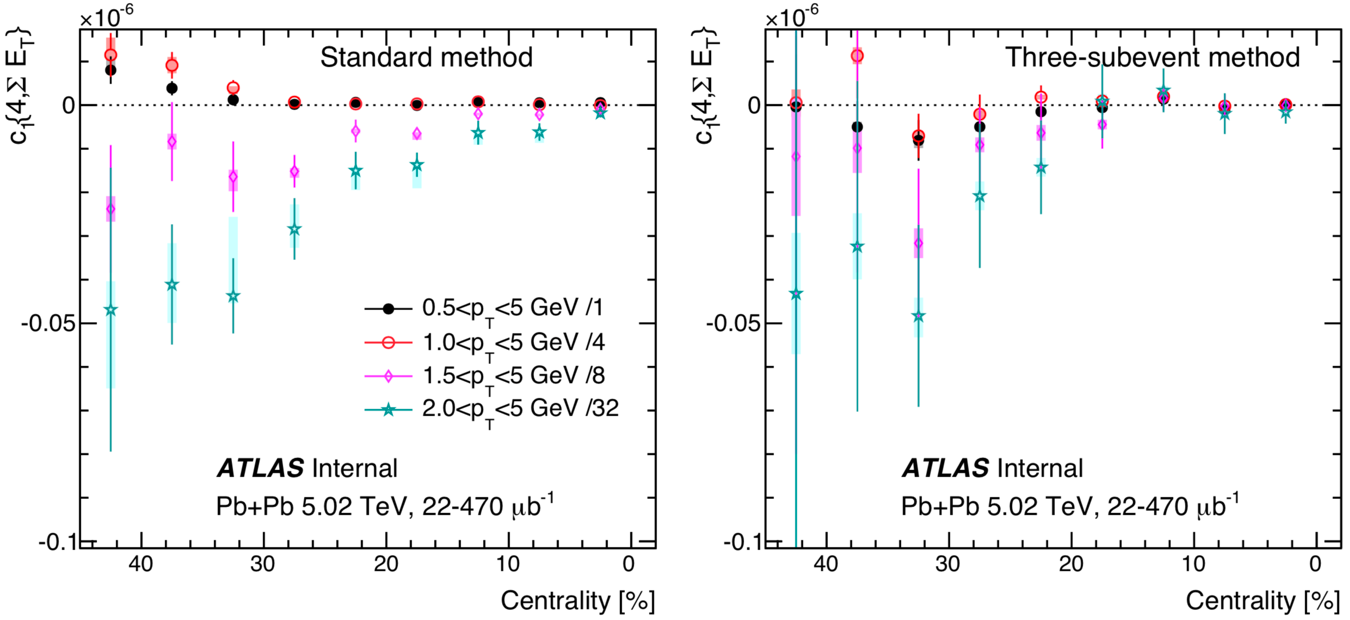
\includegraphics[width=.8\linewidth]{figs/sec_result/forQM/mtd_c4_v1.png}
\caption{4-particle cumulant $c_1\{4\}$ calculated using standard cumulant method (left) and 3-subevent method (right).}
\label{fig:mtd_c4_v1}
\end{figure}
To check whether negative $c_1\{4\}$ is caused by non-flow effects, measurement is repeated using 3-subevent method, as previously shown in Fig.~\ref{fig:mtd_c4_v1}. In addition, $c_1\{4\}$ with high $p_\text{T}$ cut is always negative in peripheral, regardless of event class definitions (shown in the paper draft~\cite{Jia:2311860}). This further supports our claim that this observation is due to genuine $v_1$ fluctuation, not other trivial effects.

\begin{figure}[H]
\centering
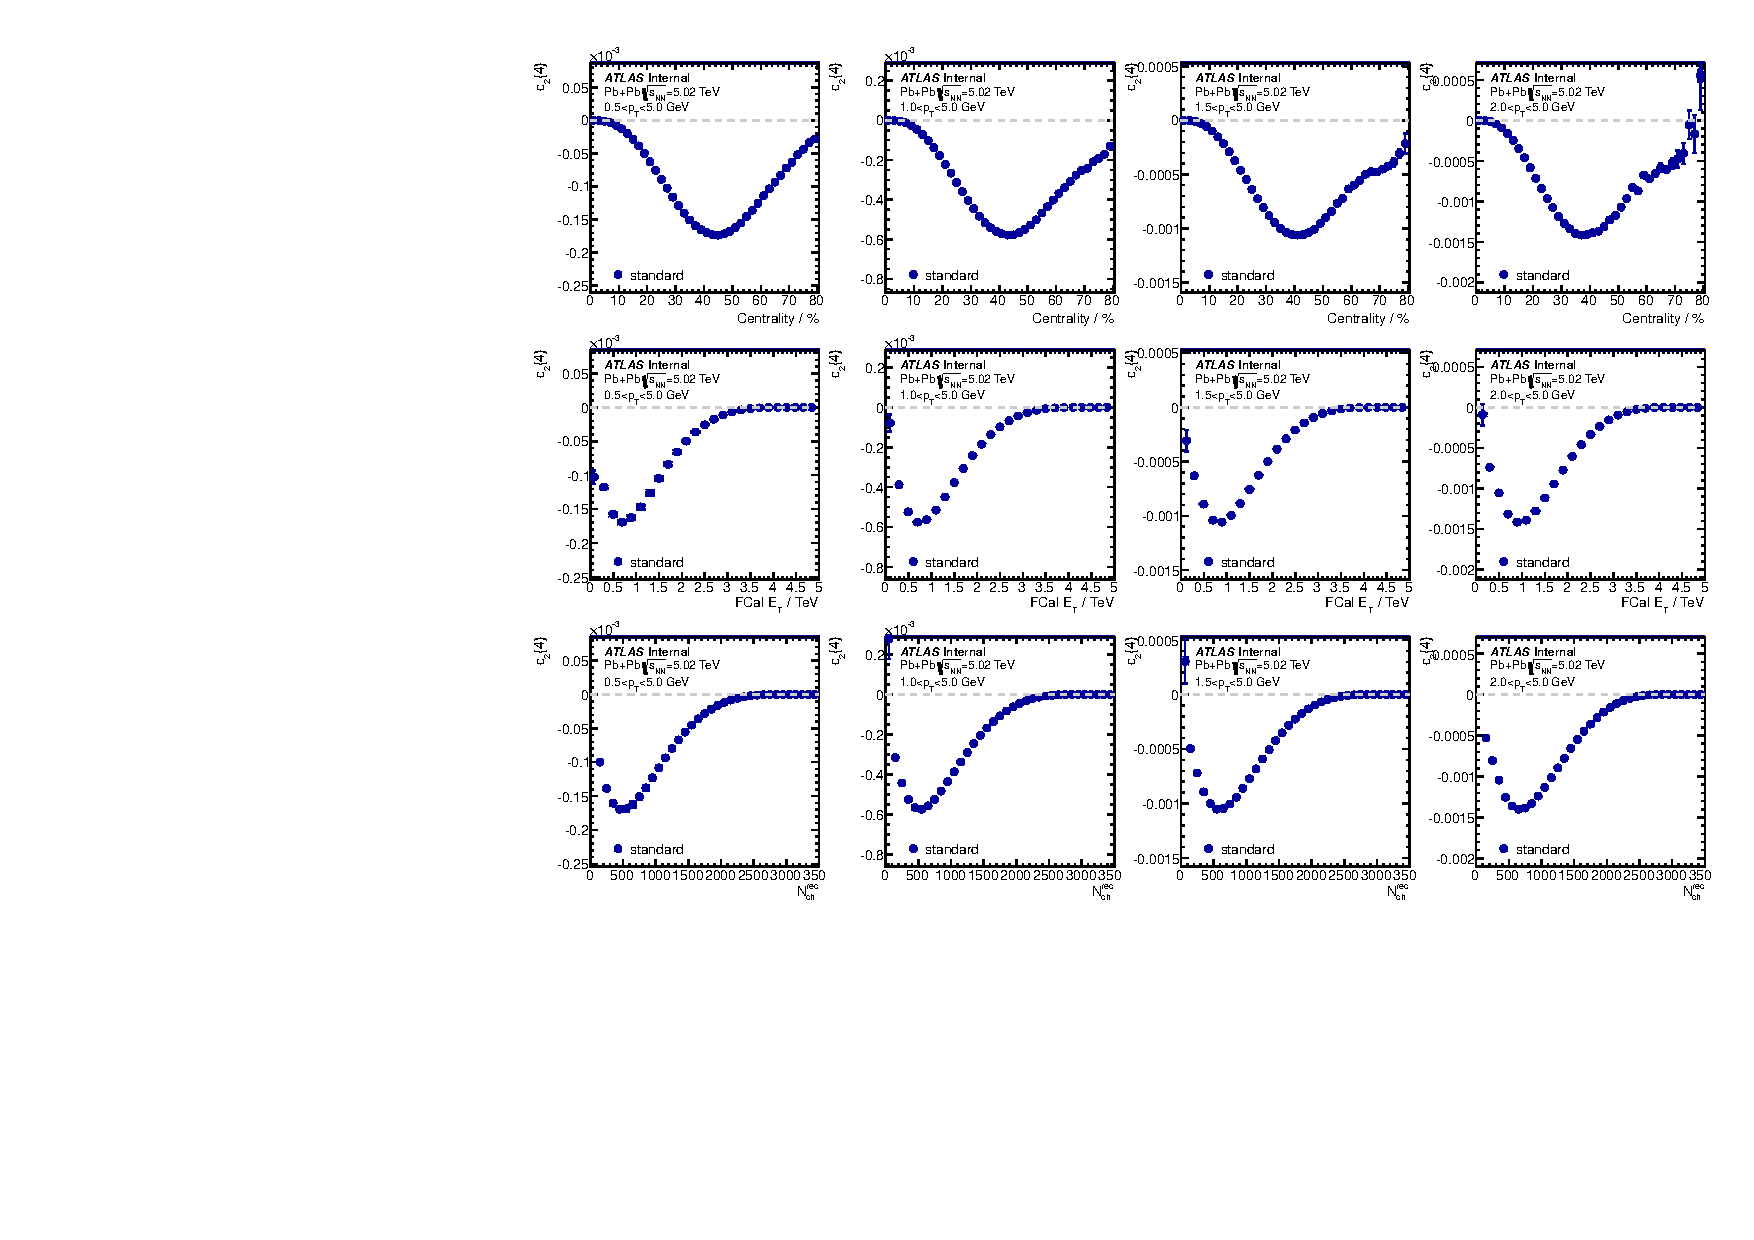
\includegraphics[width=.95\linewidth]{figs/sec_result/forQM/phy_c4_Har2.pdf}
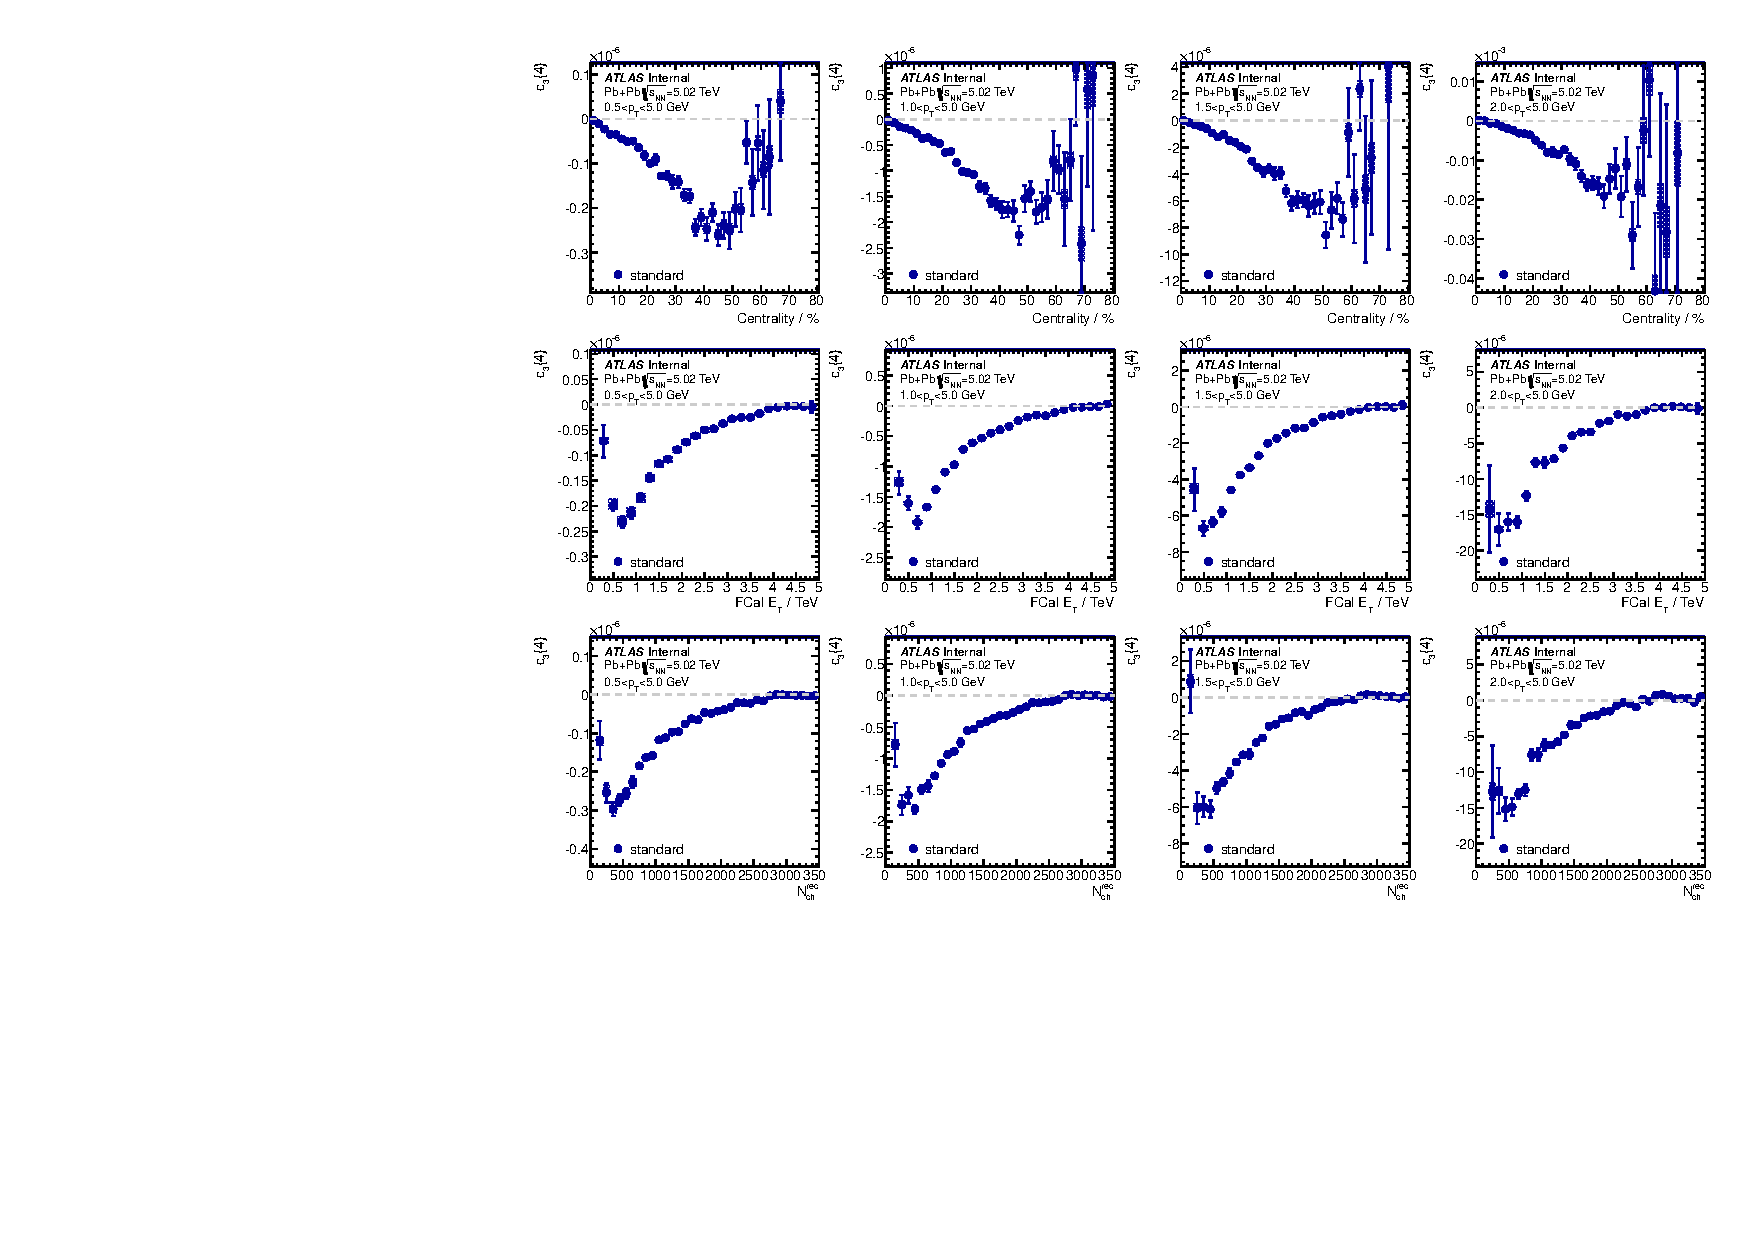
\includegraphics[width=.95\linewidth]{figs/sec_result/forQM/phy_c4_Har3.pdf}
\caption{4-particle cumulant $c_2\{4\}$ (top half) and $c_3\{4\}$ (bottom half) calculated with different $p_\text{T}$ ranges (columns) and different event class definitions (rows).}
\label{fig:result_phy_c4_Har23}
\end{figure}
Fig.~\ref{fig:result_phy_c4_Har23} present 4-particle cumulant $c_2\{4\}$ and $c_3\{4\}$ calculated with different $p_\text{T}$ ranges and different event class definitions. Both $c_2\{4\}$ and $c_3\{4\}$ follow similar centrality dependence: they start with small value, reach maximum around $40\%$ centrality, then decrease towards peripheral. Unlike the 2-particle correlation measurements, where $c_2\{2\}$ does not reach 0 in most central collision. The reason why $c_2\{4\}$ and $c_3\{4\}$ are close to 0 is driven by the flow fluctuation. In central collision, due to a large number of sources, the flow fluctuations approach Gaussian, which results in a close-to-0 4-particle cumulant. We will come back to this feature when discussing the normalized cumulant results.

As minimum $p_\text{T}$ cut increases from 0.5 to 2.0 GeV, the magnitudes of $c_2\{4\}$ and $c_3\{4\}$ increase rapidly. This $p_\text{T}$ dependence is qualitatively consistent with observations from 2-particle correlation measurements, which indicates that the fluctuations of $v_2$ and $v_3$ are so close to Gaussian, that the 4-particle cumulants are driven by the mean value of flow. We will verify this point by universality check of flow fluctuations.

\begin{figure}[H]
\centering
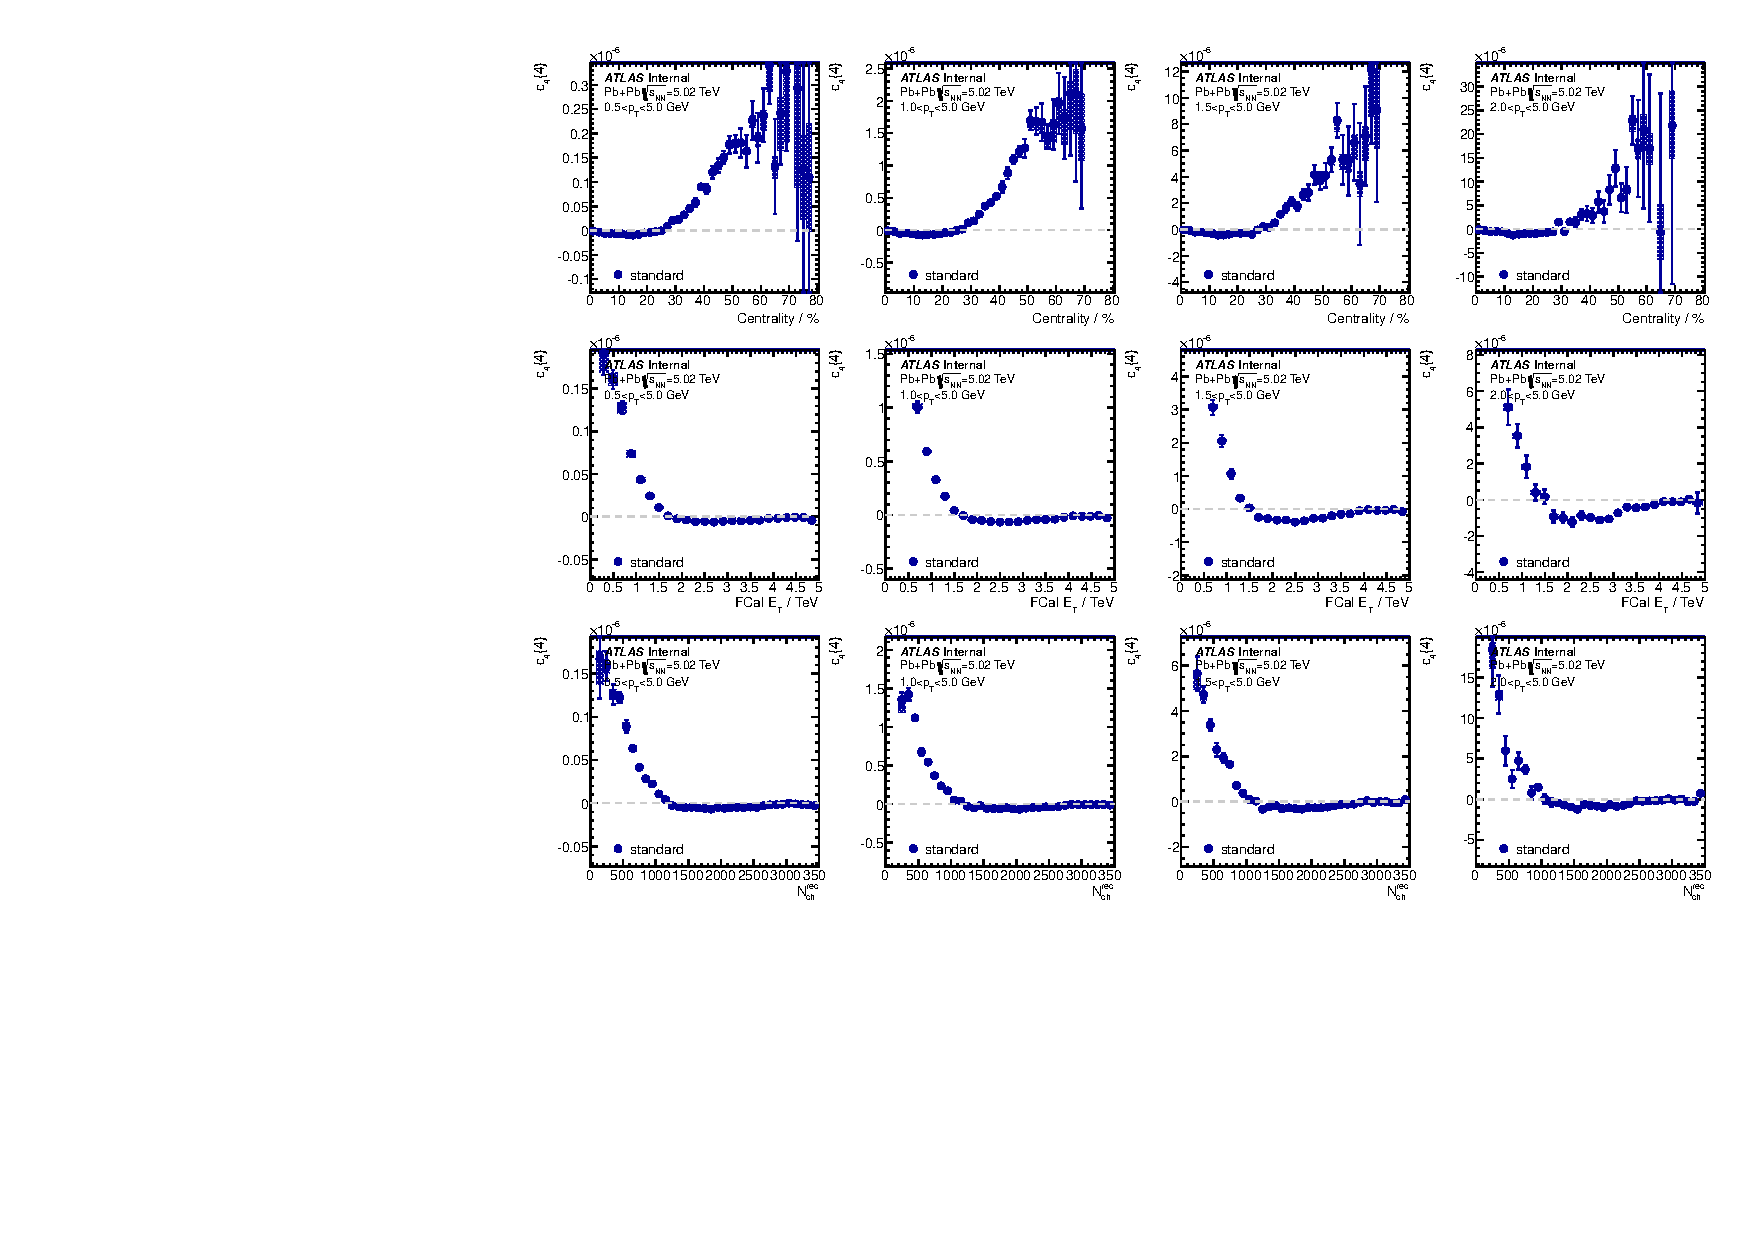
\includegraphics[width=.95\linewidth]{figs/sec_result/forQM/phy_c4_Har4.pdf}
\caption{4-particle cumulant $c_4\{4\}$ calculated with different $p_\text{T}$ ranges (columns) and different event class definitions (rows).}
\label{fig:result_phy_c4_Har4}
\end{figure}

$c_4\{4\}$ with different $p_\text{T}$ ranges are summarized in Fig.~\ref{fig:result_phy_c4_Har4}. Like $c_2\{4\}$ and $c_3\{4\}$, $c_4\{4\}$ shows strong $p_\text{T}$ dependence. It is also interesting to note that $c_4\{4\}$ is negative for centrality $<25\%$, then it turns positive and keeps increasing towards peripheral. This behavior is consistent with the hydrodynamic prediction: negative $c_4\{4\}$ in central and mid-central is due to the linear component of $v_4$, while in peripheral, the non-linear component from $v_2^2$ dominates over linear component:
\begin{equation}
v_4 = v_{4L} + k v_2^2
\end{equation}
and this non-linear component causes $v_4$ fluctuation to be non-Gaussian, which results in positive $c_4\{4\}$ (note that 4-particle cumulant is ill-defined if it's positive). By checking different event class definitions, it's also clear that the balance between linear and non-linear is not due to centrality fluctuation.

\begin{figure}[H]
\centering
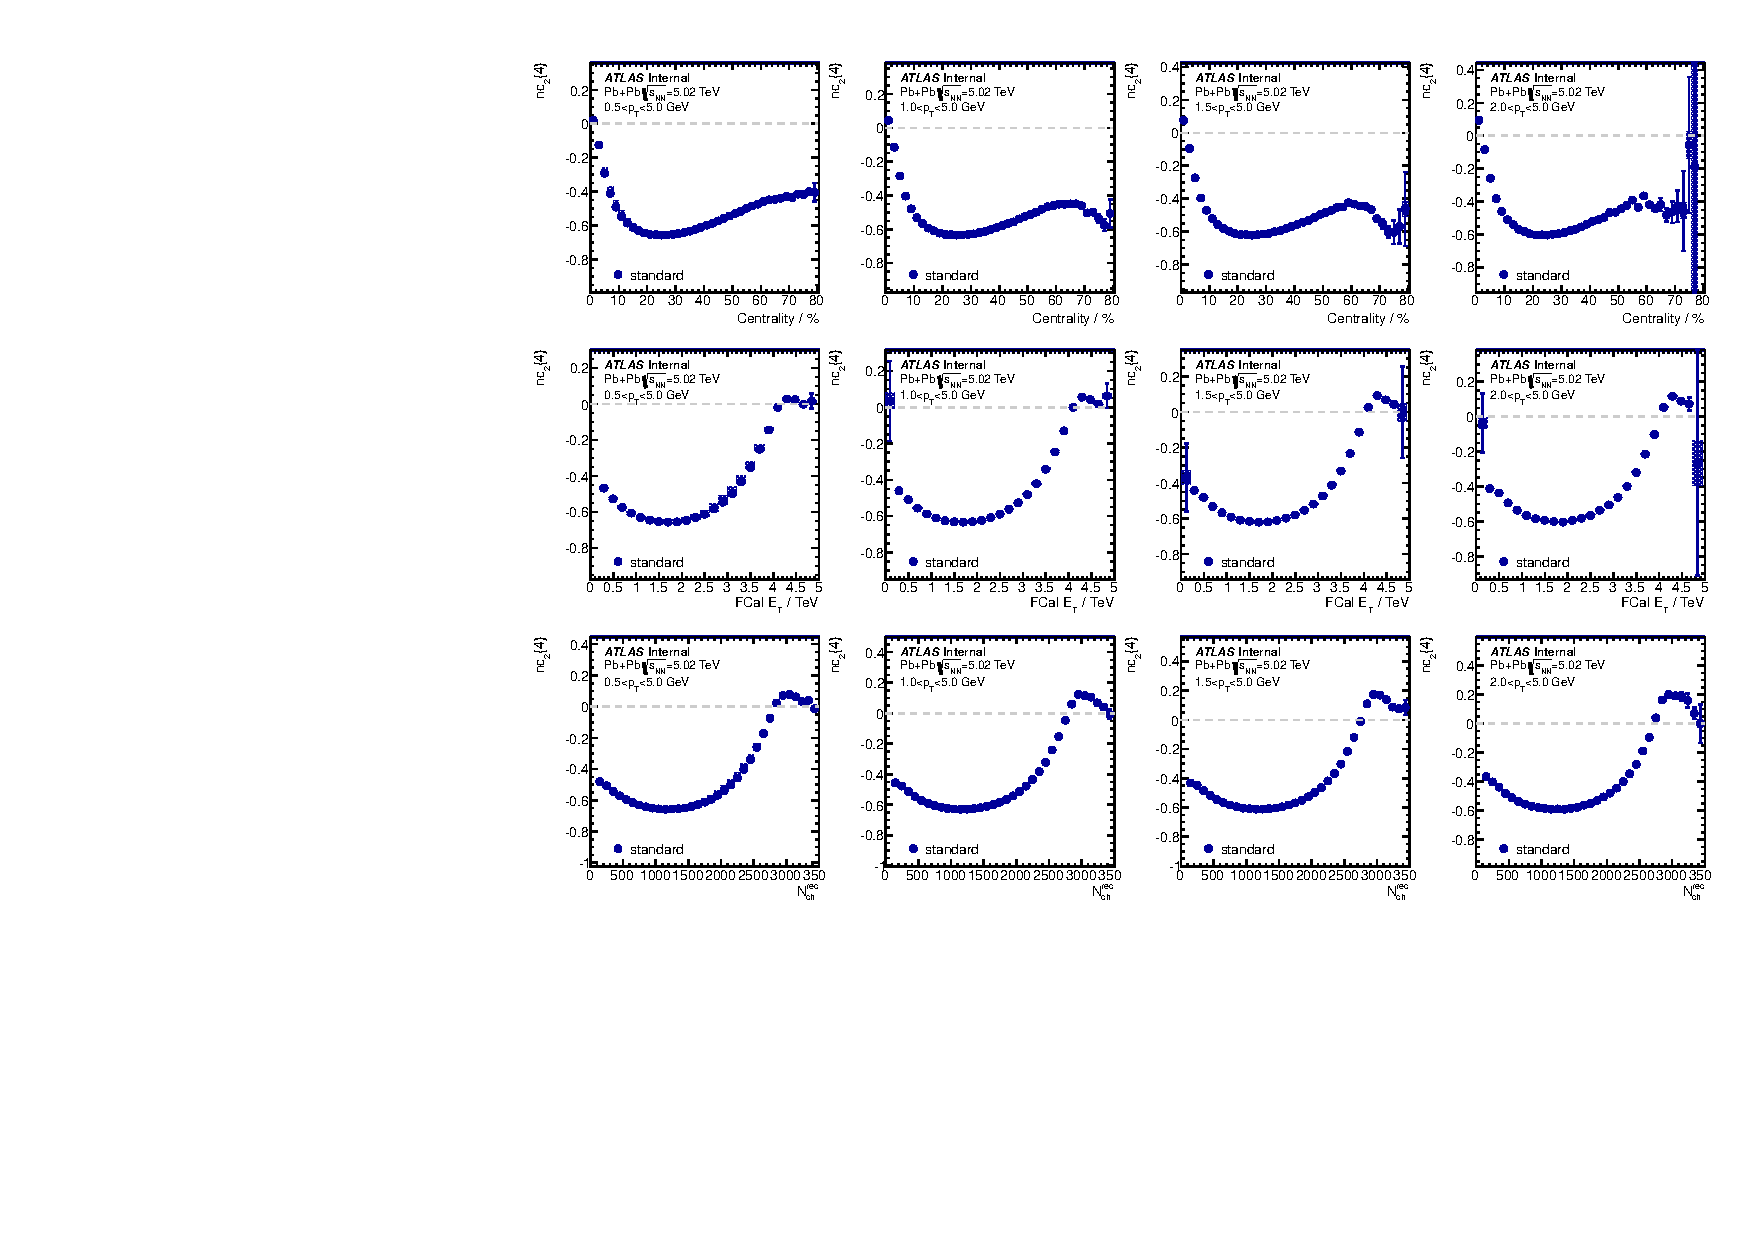
\includegraphics[width=.95\linewidth]{figs/sec_result/forQM/phy_nc4_Har2.pdf}
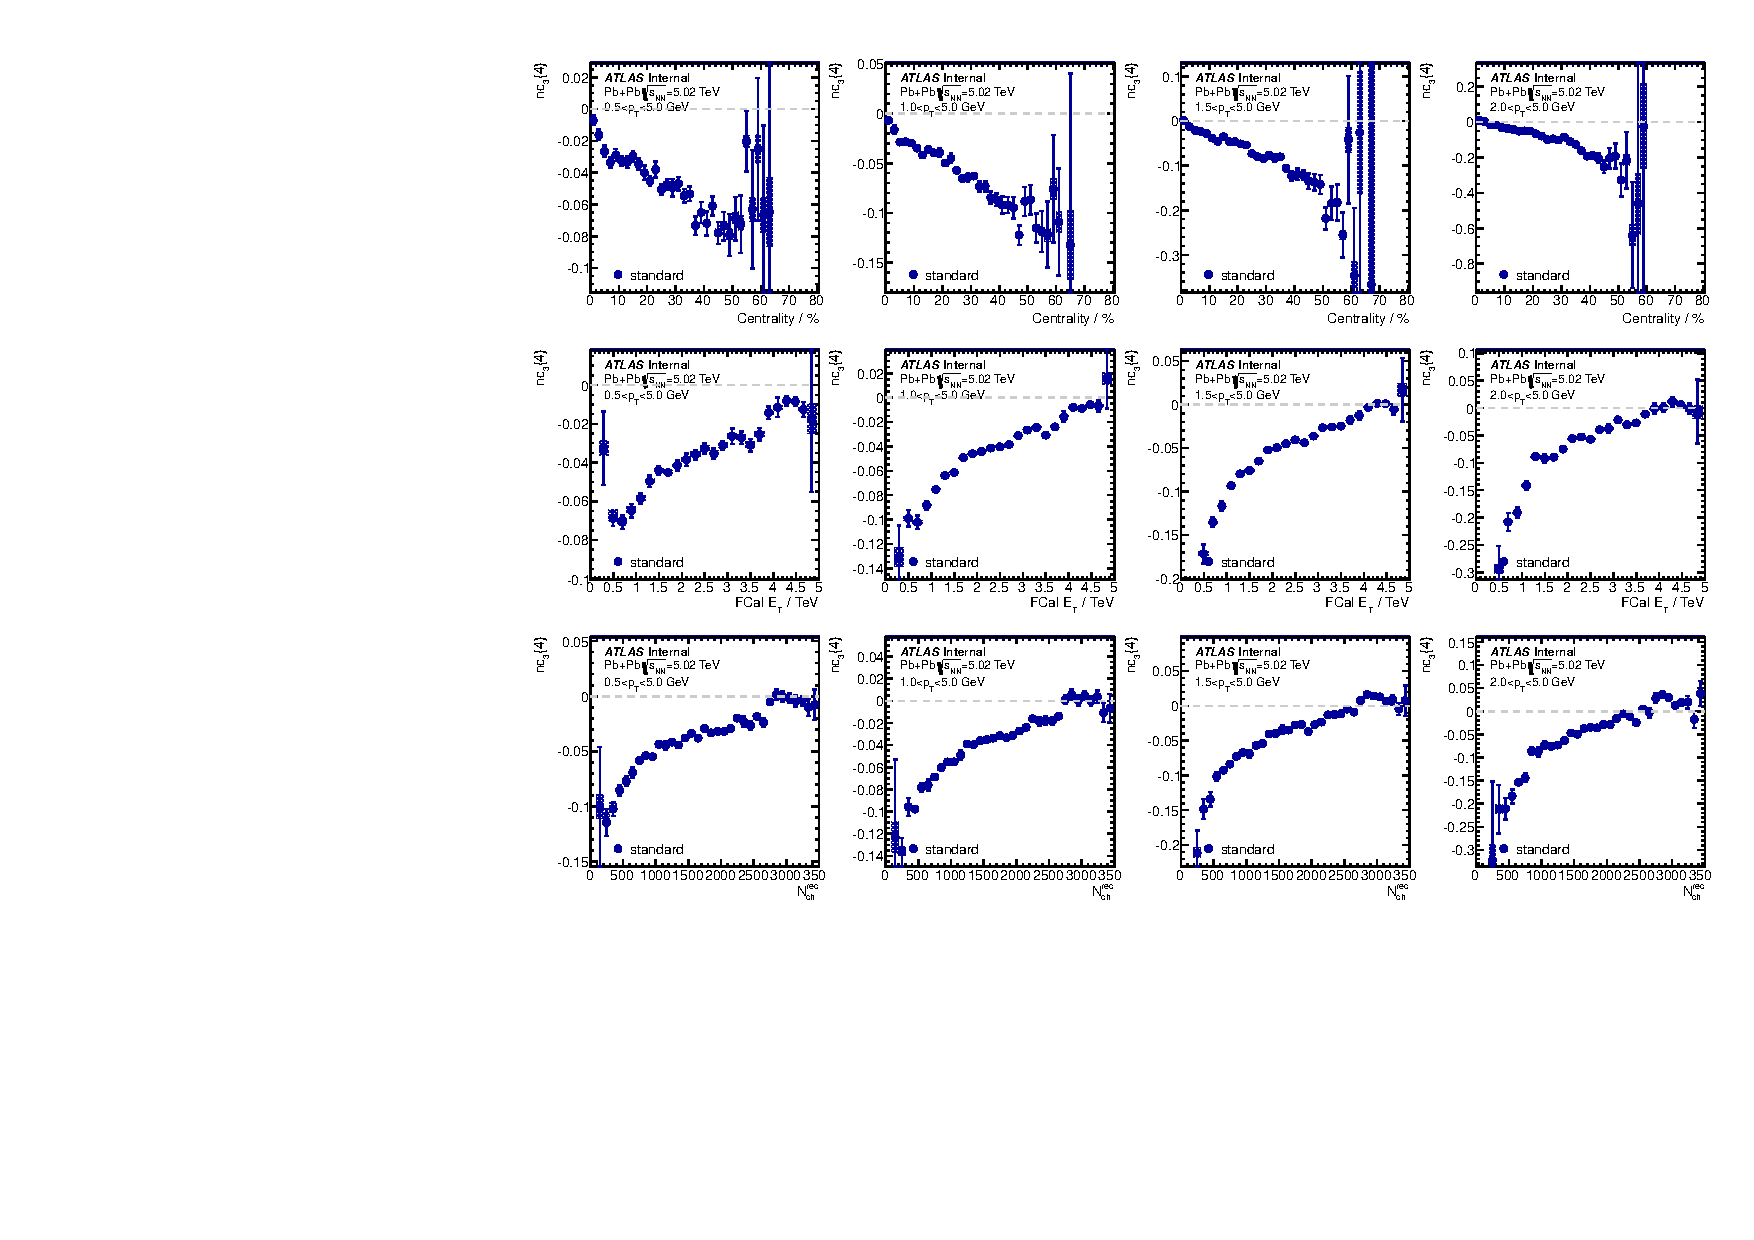
\includegraphics[width=.95\linewidth]{figs/sec_result/forQM/phy_nc4_Har3.pdf}
\caption{Normalized 4-particle cumulant $nc_2\{4\}$ and $nc_3\{4\}$ calculated with different $p_\text{T}$ ranges (columns) and different event class definitions (rows).}
\label{fig:result_phy_nc4_Har23}
\end{figure}
In order to show the fluctuation nature of flow harmonics, Fig.~\ref{fig:result_phy_nc4_Har23} presents the similar results but with normalized cumulants $nc_2\{4\}$ and $nc_3\{4\}$. By dividing out 2-particle correlations from 4-particle cumulant, normalized cumulant focuses on the fluctuation itself. For $v_2$, the fluctuation is largest in mid-centrality $20-30\%$ and it decreases towards central and peripheral. In the ultra-central collision with centrality $<1\%$, $nc_2\{4\}$ exhibits rich sign change behavior: it first reach 0 then becomes positive, in the most-central collisions, it drops back to 0. This behavior can be explained with centrality fluctuation, which we will dive into in details in the next section. For $v_3$, since there is no average geometry from the initial stage, the fluctuation nature is very different from $v_2$: magnitude of $\hat{3}\{4\}$ keeps increasing towards peripheral. This is expected because the number of sources drops quickly as collision moves to peripheral. Meanwhile, like $v_2$, $nc_3\{4\}$ quickly approaches 0 in central collision, however, in most cases, it does not change sign as $nc_2\{4\}$, expect for the $N_{ch}^{rec}$ binned cases with very high $p_\text{T}$ cuts. Finally, it is also noted that the $p_\text{T}$ dependence for normalized cumulant is much weaker than cumulant, indicating that the flow fluctuation has a weak $p_\text{T}$ dependence.

\begin{figure}[H]
\centering
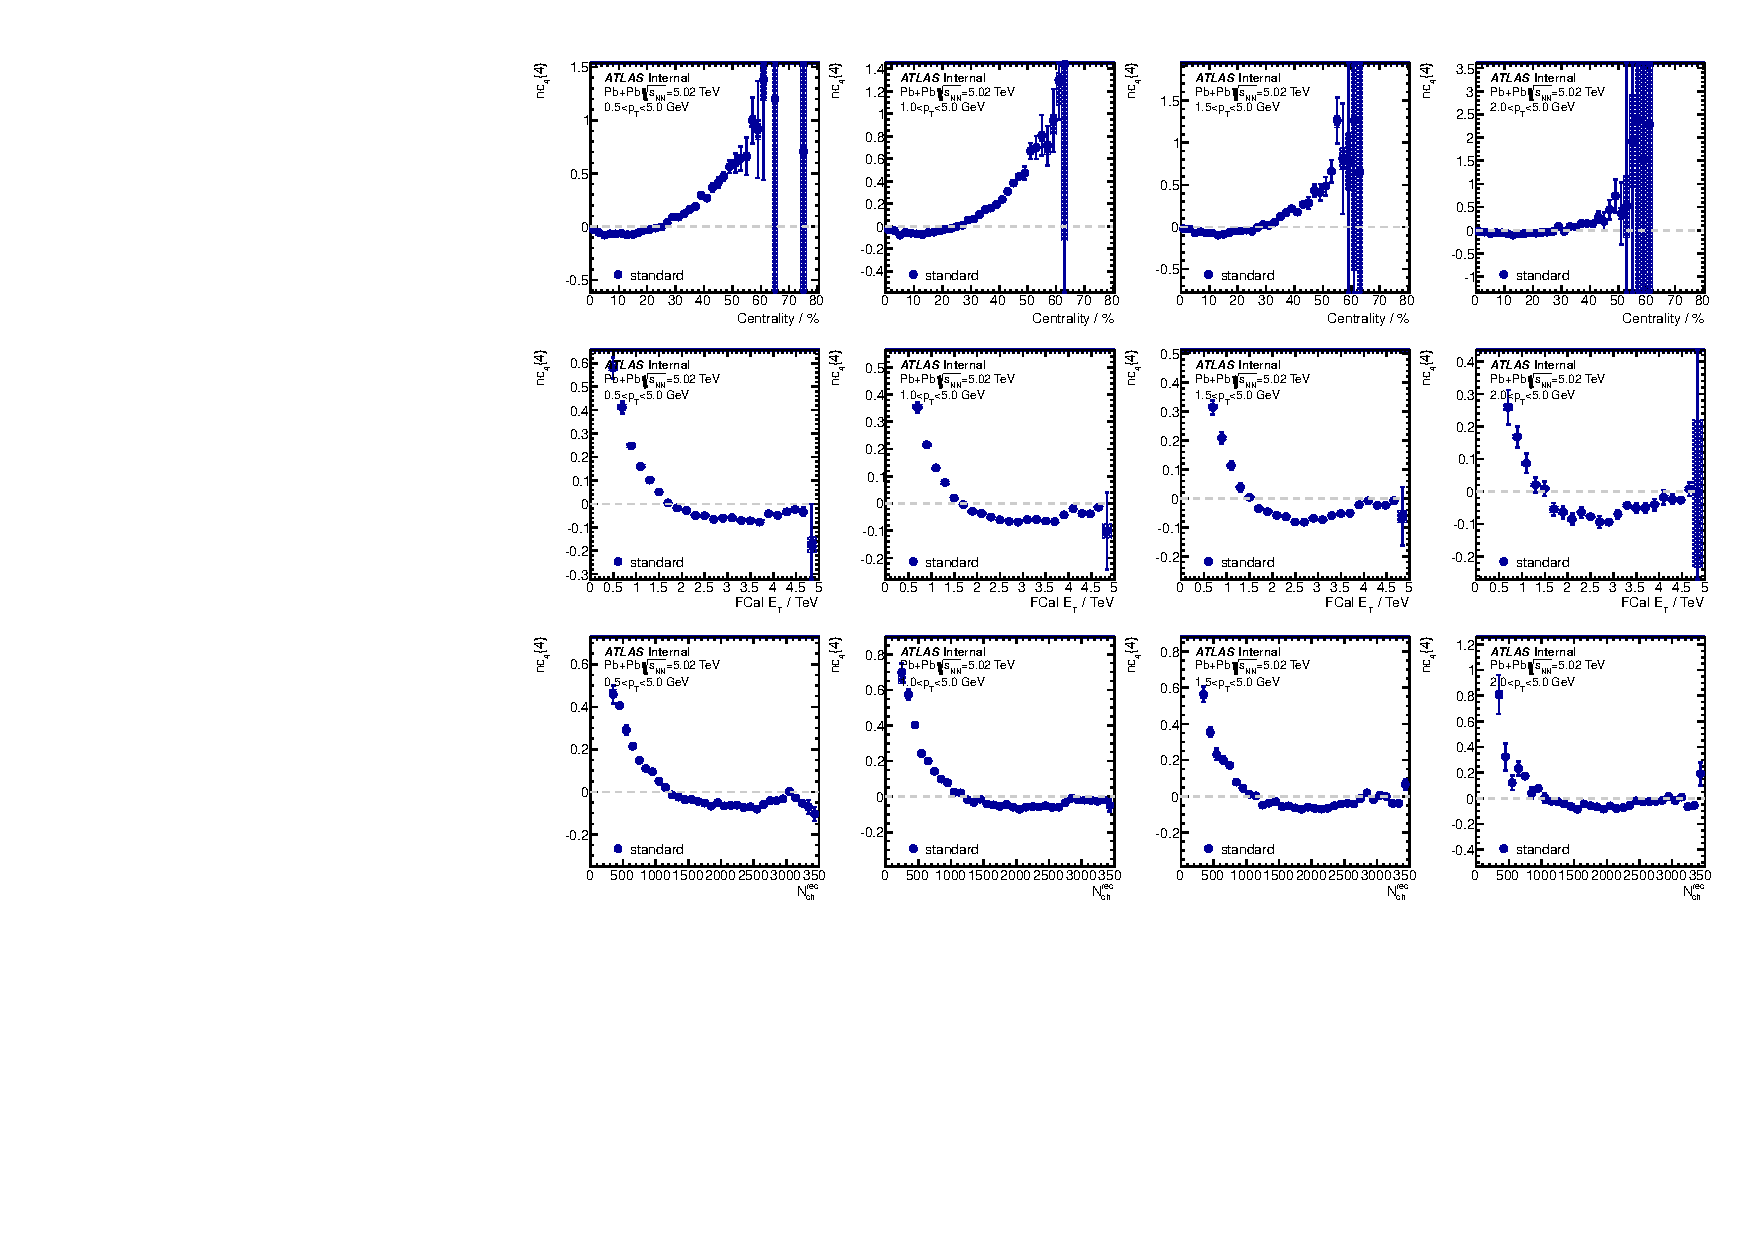
\includegraphics[width=.95\linewidth]{figs/sec_result/forQM/phy_nc4_Har4.pdf}
\caption{Normalized 4-particle cumulant $nc_4\{4\}$ calculated with different $p_\text{T}$ ranges (columns) and different event class definitions (rows).}
\label{fig:result_phy_nc4_Har4}
\end{figure}
Fig.~\ref{fig:result_phy_nc4_Har4} shows the normalized 4-particle cumulant $nc_4\{4\}$, where the negative trend in central and mid-central is more obvious than without normalization. This is actually the advantage of normalizing cumulant: fluctuation behaviors can be easily spotted without zooming in.

\subsection{4-particle cumulant in ultra-central collisions}
Follow the discussions in previous sections, magnitudes of $c_2\{4\}$ and $c_3\{4\}$ approach 0 towards central collisions, due to the increase of the number of sources. In Run 2 5.02 TeV Pb+Pb, ultra-central collision triggers are applied to enhance the statistics for events with centrality $<1\%$(See Section.~\ref{sec:evtSel}). With abundant statistics seeded by the UCC triggers, it provides a great opportunity to study the cumulant in ultra-central collisions. In this section, we are plotting $c_2\{4\}$, which has the largest signal, as function of FCal $E_\text{T}$ instead of centrality. It worth mentioning that the event class is also defined with FCal $E_\text{T}$, with bin width $=20$ GeV.

Fig.~\ref{fig:PbPb502_UCC_FCal_v2_mtd} presents the $c_2\{4\}$ in ultra-central Pb+Pb collisions, calculated with both cumulant methods. $c_2\{4\}$ from 3-subevent is systematically lower, even though within statistical uncertainties. This is because in large systems, the non-flow contributions are already largely suppressed with 4-particle cumulants. For lower $p_\text{T}$ range $0.5<p_\text{T}<5.0$ GeV (left plot), $c_2\{4\}$ is negative for FCal $E_\text{T}<4.1$ TeV, which picks up the tail of $c_2\{4\}$ as a function of centrality (Fig.~\ref{fig:result_phy_c4_Har23}). As FCal $E_\text{T}$ increases, $c_2\{4\}$ changes the sign at $E_\text{T}=4.2$ TeV and stays positive for $E_\text{T}<4.6$ TeV. For $E_\text{T}>4.6$ TeV, $c_2\{4\}$ is back to 0 again. The positive sign of $c_2\{4\}$ is very interesting, since with increasing number of sources, the $v_2$ fluctuation should approach Gaussian, which results in $c_2\{4\}=0$. However, as shown in this figure, this is actually not the case: $c_2\{4\}$ can be positive in ultra-central collision, with more than 3-sigma statistical significance. For the higher $p_\text{T}$ range $1.8<p_\text{T}<5.0$ GeV, trends are similar as lower $p_\text{T}$ range, but the magnitude of positive $c_2\{4\}$ becomes larger with $p_\text{T}$.
\begin{figure}[H]
\centering
\includegraphics[width=.45\linewidth]{figs/sec_result/PbPb502_UCC/PbPb502_mtd_Har2_pt0.pdf}
\includegraphics[width=.45\linewidth]{figs/sec_result/PbPb502_UCC/PbPb502_mtd_Har2_pt5.pdf}
\caption{$c_2\{4\}$ in 5.02 TeV ultra-central Pb+Pb, calculated with different cumulant methods. Event class is defined by FCal $E_\text{T}$. Left panel is for the lower $p_\text{T}$ range and right panel is for the higher $p_\text{T}$ range.}
\label{fig:PbPb502_UCC_FCal_v2_mtd}
\end{figure}

To directly show the $p_\text{T}$ dependence of $c_2\{4\}$ in ultra-central collisions, Fig.~\ref{fig:PbPb502_UCC_FCal_v2_pT} presents the $c_2\{4\}$ calculated in different $p_\text{T}$ ranges, with standard cumulant method. It is noticed that $c_2\{4\}$ from all the $p_\text{T}$ ranges follow similar trend: $c_2\{4\}$ starts with negative, turns positive around $E_\text{T}=4.1$ TeV, and drops back to 0 in most central collisions. The maximum magnitude of $c_2\{4\}$ increases quickly as minimum $p_\text{T}$ cut increases.
\begin{figure}[H]
\centering
\includegraphics[width=.45\linewidth]{figs/sec_result/PbPb502_UCC/PbPb502_pT_1sub_Har2.pdf}
\includegraphics[width=.45\linewidth]{figs/sec_result/PbPb502_UCC/PbPb502_pT_1sub_Har3.pdf}
\caption{$c_2\{4\}$ and $c_3\{4\}$ in 5.02 TeV Pb+Pb, with event class binned with FCal $E_\text{T}$. Results are calculated in different $p_\text{T}$ ranges, with standard cumulant method.}
\label{fig:PbPb502_UCC_FCal_v2_pT}
\end{figure}

The definition of event class is important in cumulant measurement. Since cumulant measures the underlying $v_n$ probability distribution within a bunch of similar events, by changing the event class definition, the magnitude, even the sign of cumulant could also change. In order to check whether the positive $c_2\{4\}$ observed in ultra-central collision is due to such binning effects, in this section, a different event class definition is applied: events are grouped according to their $N_{ch}^{rec}$, with $0.5<p_\text{T}<5.0$ GeV. To properly compare with FCal $E_\text{T}$ binning, the final results are mapped to the mean value of FCal $E_\text{T}$ for each $N_{ch}^{rec}$ bin.

The result is shown in Fig.~\ref{fig:PbPb502_UCC_FCal_v2_mtd}, with particles from lower and higher $p_\text{T}$ ranges separately. $c_2\{4\}$ from 3-subevent is systematically lower, even though still within statistical uncertainties. Compared with FCal $E_\text{T}$ binning, similar trend is observed: $c_2\{4\}$ starts with negative value, becomes positive, and drops back to 0 in the most central collisions. However, there are two major differences between the two event class definitions:
\begin{itemize}
\item the maximum magnitude depends on event class definition;
\item the point where $c_2\{4\}$ changes sign depends on event class definition;
\end{itemize}
which is not surprising since the $c_2\{4\}$ signal in ultra-central collision is small, and slight changes in event class definition will modify the $v_2$ fluctuation, which leads to the observations mentioned above. However, it is interesting that even though the magnitude of maximum $c_2\{4\}$ changes a lot, the trends of $c_2\{4\}$ from two event class definitions are still similar.

\begin{figure}[H]
\centering
\includegraphics[width=.45\linewidth]{figs/sec_result/PbPb502_UCC_Nch/PbPb502_mtd_Har2_pt0.pdf}
\includegraphics[width=.45\linewidth]{figs/sec_result/PbPb502_UCC_Nch/PbPb502_mtd_Har2_pt5.pdf}
\caption{$c_2\{4\}$ in 5.02 TeV ultra-central Pb+Pb, calculated with different cumulant methods. Event class is defined by $N_{ch}$. Left panel is for the lower $p_\text{T}$ range and right panel is for the higher $p_\text{T}$ range.}
\label{fig:PbPb502_UCC_FCal_v2_mtd}
\end{figure}

To directly show the $p_\text{T}$ dependence of $c_2\{4\}$ in ultra-central collisions, Fig.~\ref{fig:PbPb502_UCC_Nch_v2_pT} presents the $c_2\{4\}$ calculated in different $p_\text{T}$ ranges, with standard cumulant method. It is observed that $c_2\{4\}$ from all the $p_\text{T}$ ranges follow similar trend: $c_2\{4\}$ starts with negative, turns positive, and drops back to 0 in most-central collisions. The maximum magnitude of $c_2\{4\}$ increases quickly as minimum $p_\text{T}$ cut increases.
\begin{figure}[H]
\centering
\includegraphics[width=.45\linewidth]{figs/sec_result/PbPb502_UCC_Nch/PbPb502_pT_1sub_Har2.pdf}
\includegraphics[width=.45\linewidth]{figs/sec_result/PbPb502_UCC_Nch/PbPb502_pT_1sub_Har3.pdf}
\caption{$c_2\{4\}$ and $c_3\{4\}$ in 5.02 TeV Pb+Pb, with event class binned with $N_{ch}$. Results are calculated in different $p_\text{T}$ ranges, with standard cumulant method.}
\label{fig:PbPb502_UCC_Nch_v2_pT}
\end{figure}

\subsection{4-particle cumulant in 2.76 and 5.02 TeV}
\begin{figure}[H]
\centering
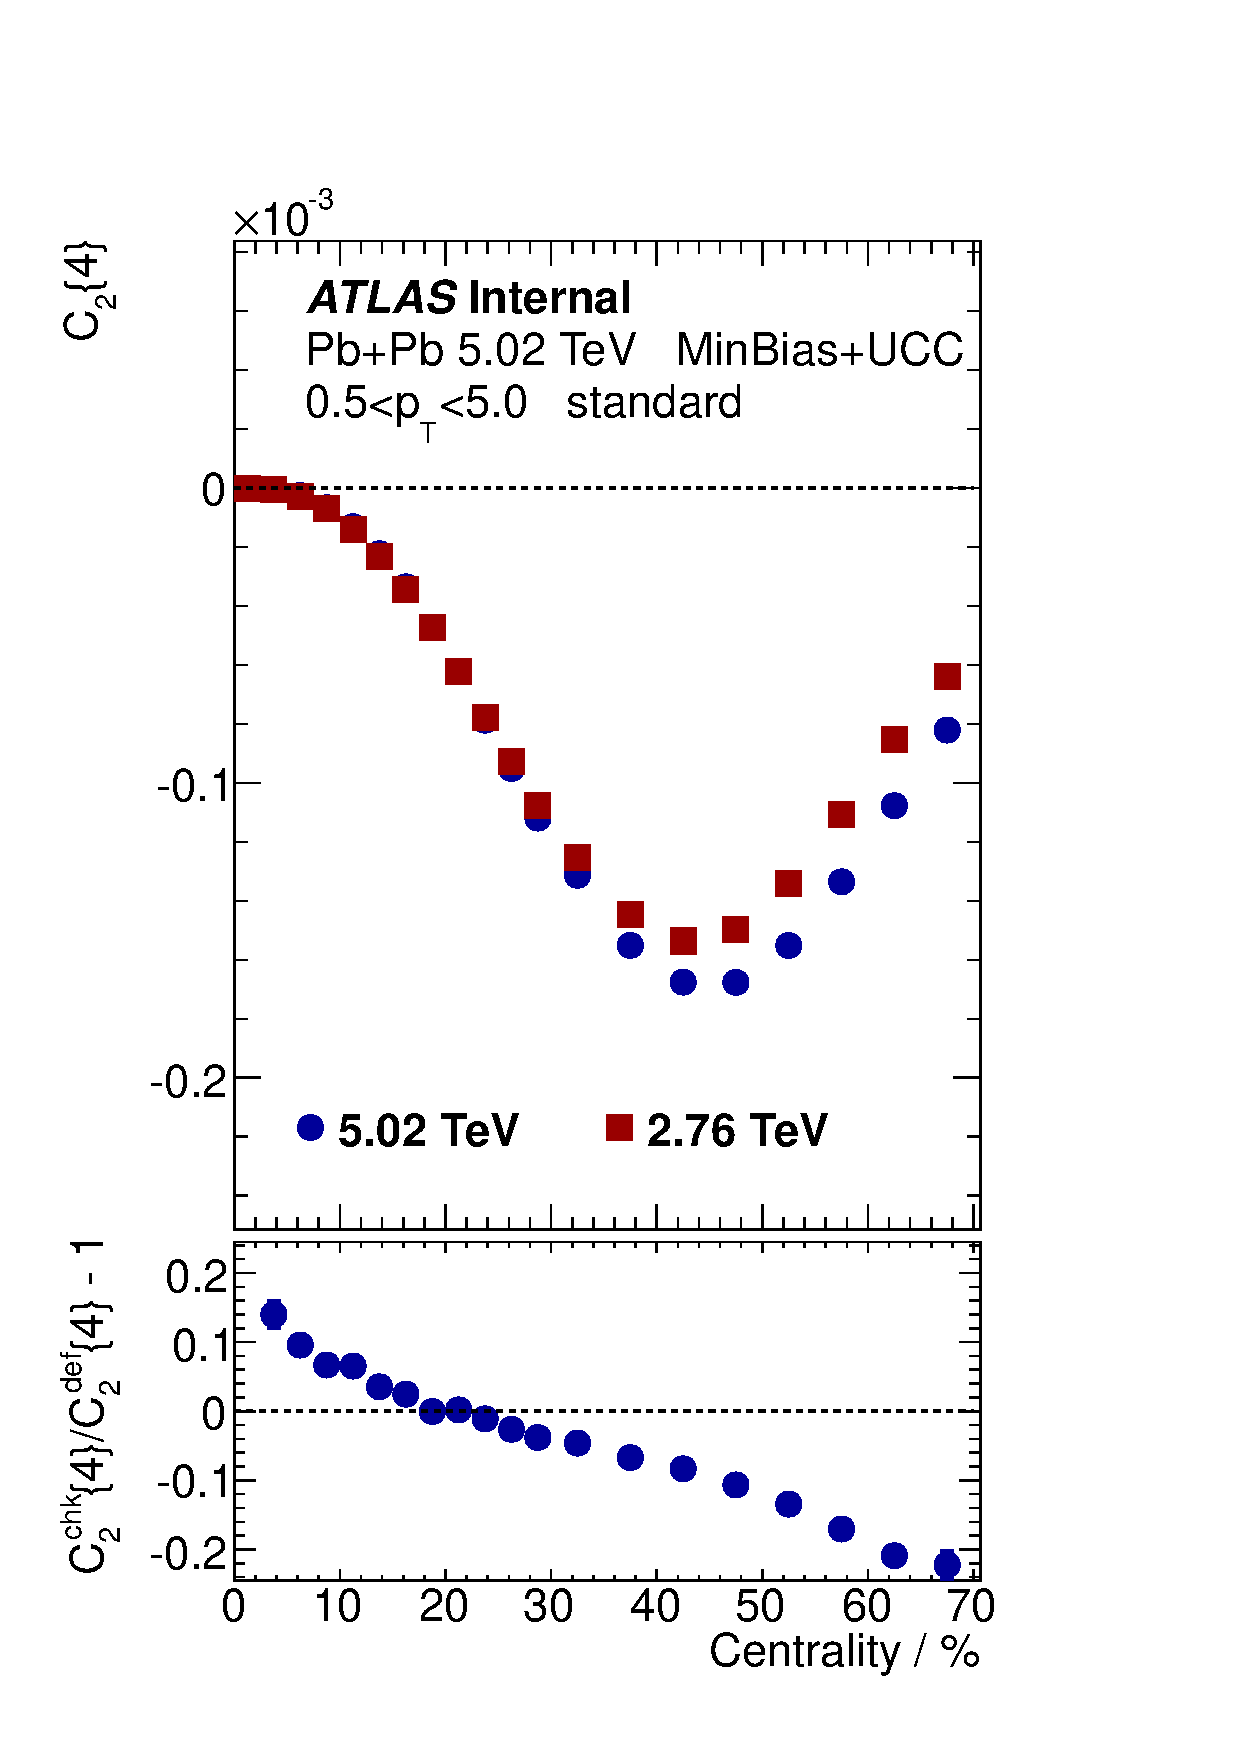
\includegraphics[width=.35\linewidth]{figs/sec_result/energyDep/PbPb502_sys1_1sub_Har2_Pt0.pdf}
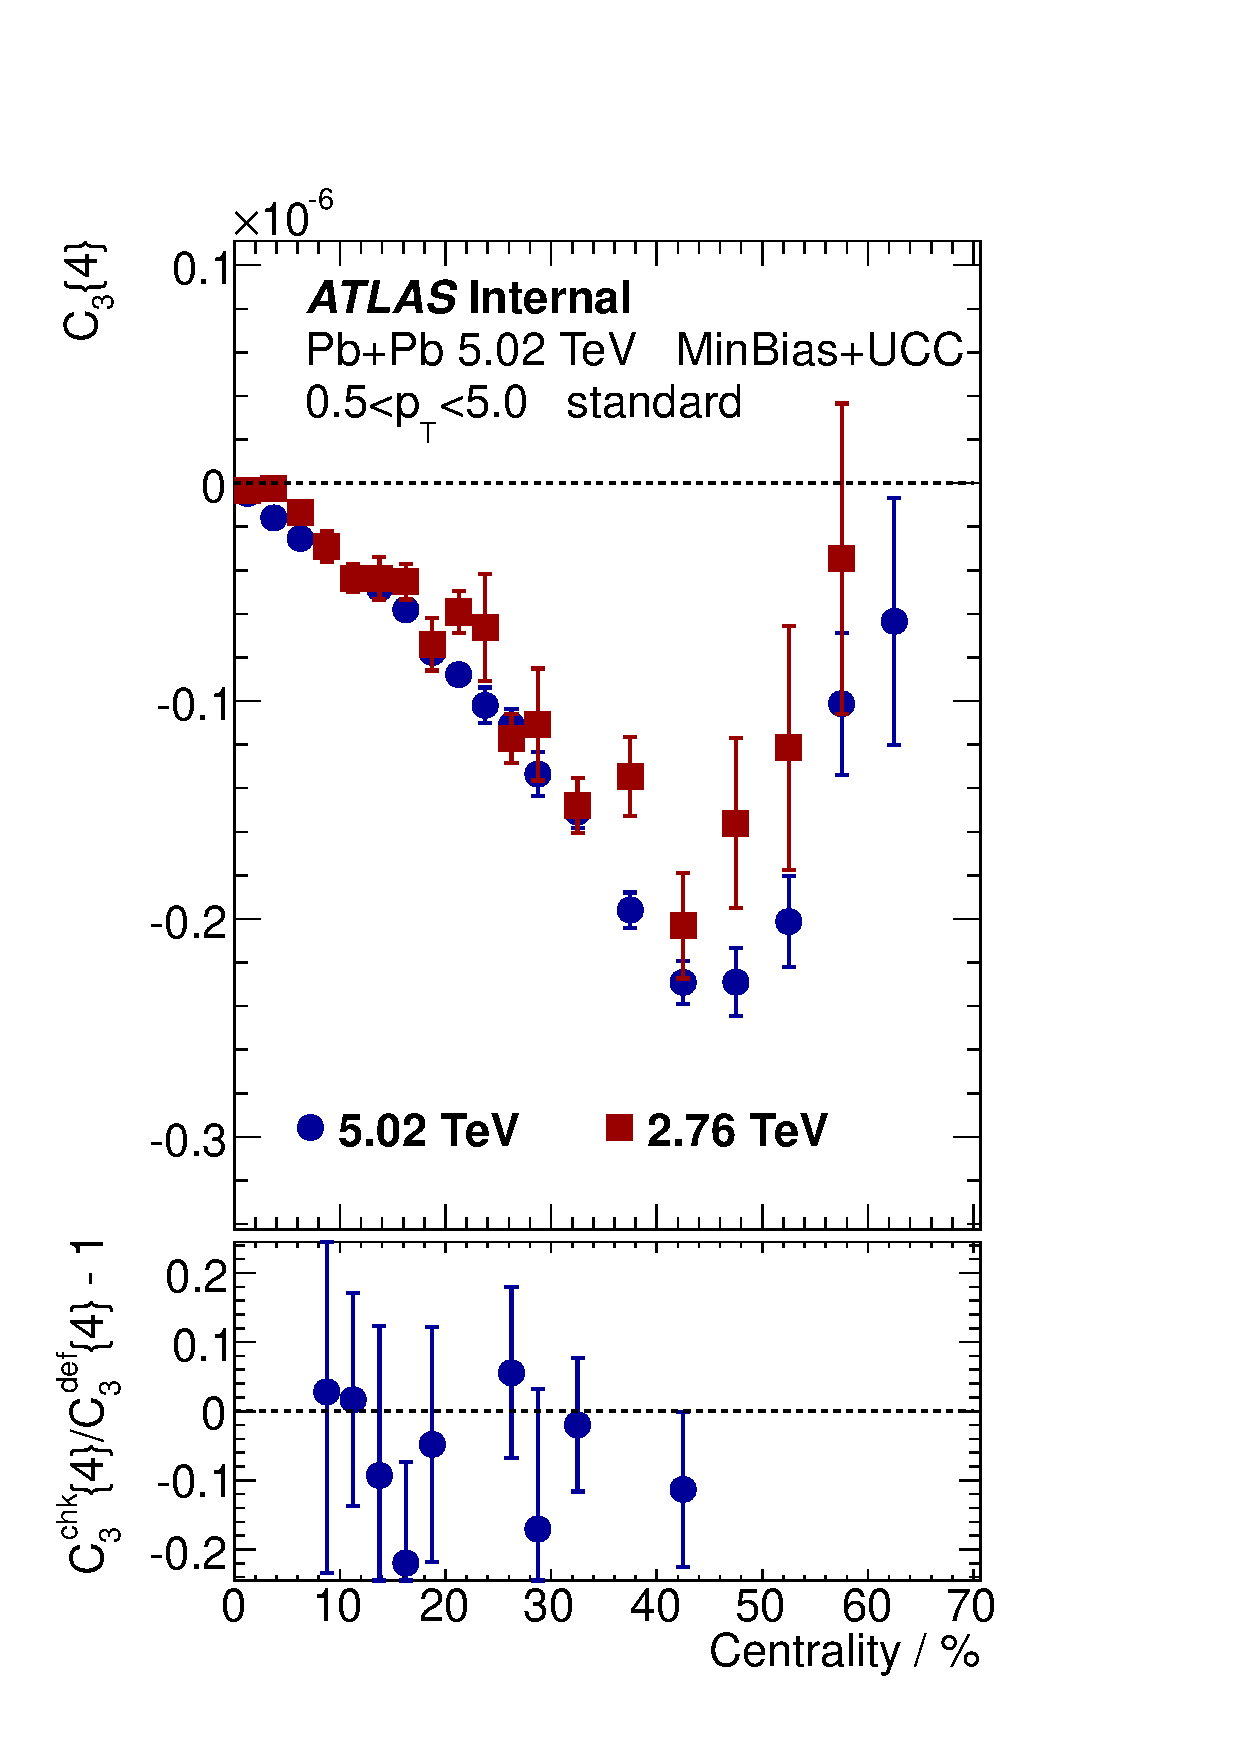
\includegraphics[width=.35\linewidth]{figs/sec_result/energyDep/PbPb502_sys1_1sub_Har3_Pt0.pdf}
\caption{$c_2\{4\}$ and $c_3\{4\}$ at 2.76 and 5.02 TeV Pb+Pb collision, calculated with standard cumulant. The bottom panels show the relative difference between 2.76 and 5.02 TeV Pb+Pb.}
\label{fig:result_energyDep}
\end{figure}
Judging from previous measurements of 2-particle correlation that discussed in Sec.~\ref{sec:pre}, we expect the 4-particle cumulant $c_n\{4\}$ is also weakly energy dependent. Fig.~\ref{fig:result_energyDep} shows the comparison of $c_2\{4\}$ and $c_3\{4\}$ between 2.76 and 5.02 TeV Pb+Pb collision, as a function of centrality. The cumulants are calculated using standard cumulant method with $0.5<p_\text{T}<5.0$ GeV. For $c_2\{4\}$, between $0\%$ and $20\%$ centrality, the magnitude of $c_2\{4\}$ in 2.76 TeV Pb+Pb is larger than 5.02 TeV. As collision goes to peripheral, the magnitude of $c_2\{4\}$ in 2.76 TeV Pb+Pb becomes smaller than 5.02 TeV. The maximum relative difference reaches about $20\%$ at most peripheral, which is around $5\%$ level if converted to $v_2\{4\}$. While for $c_3\{4\}$, the trend is simpler between two energies: magnitude of $c_3\{4\}$ at 2.76 TeV is always smaller than 5.02 TeV. The maximum relative difference is still around $~5\%$ on the $v_3\{4\}$ level. In summary, the energy dependence of $c_3\{4\}$ and $c_4\{4\}$ is weak between 2.76 and 5.02 TeV as expected. Note that it is possible that such weak energy dependence is due to the small mean $p_\text{T}$ difference, as well as the different $\eta$ distributions, between the two energies.

\subsection{6-particle cumulant $c_n\{6\}$ and $nc_n\{6\}$}
Enhancement of statistics in Run 2 makes it feasible to calculate up to 6-particle cumulant with high precision. In this section, we will show the 6-particle cumulant results for $v_2$ and $v_3$.
\begin{figure}[H]
\centering
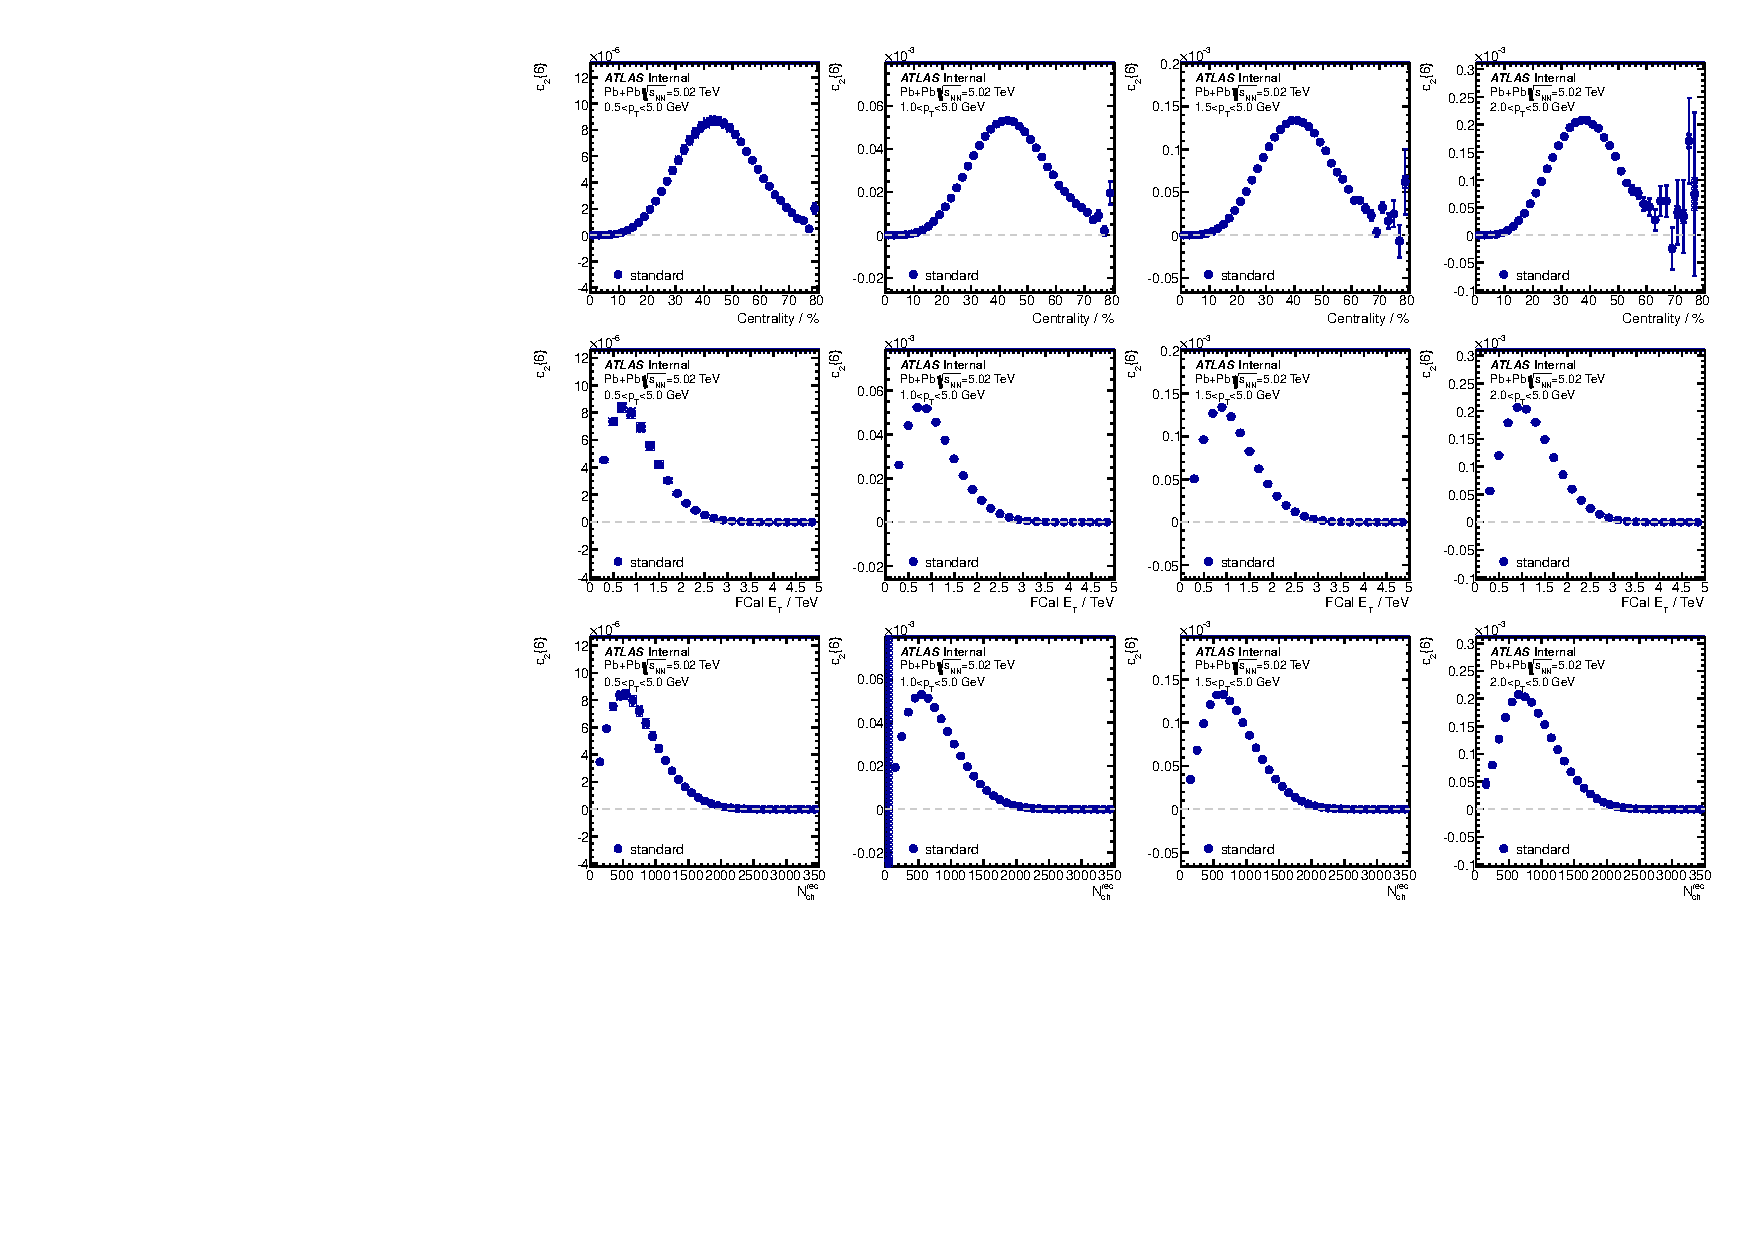
\includegraphics[width=.95\linewidth]{figs/sec_result/forQM/phy_c6_Har2.pdf}
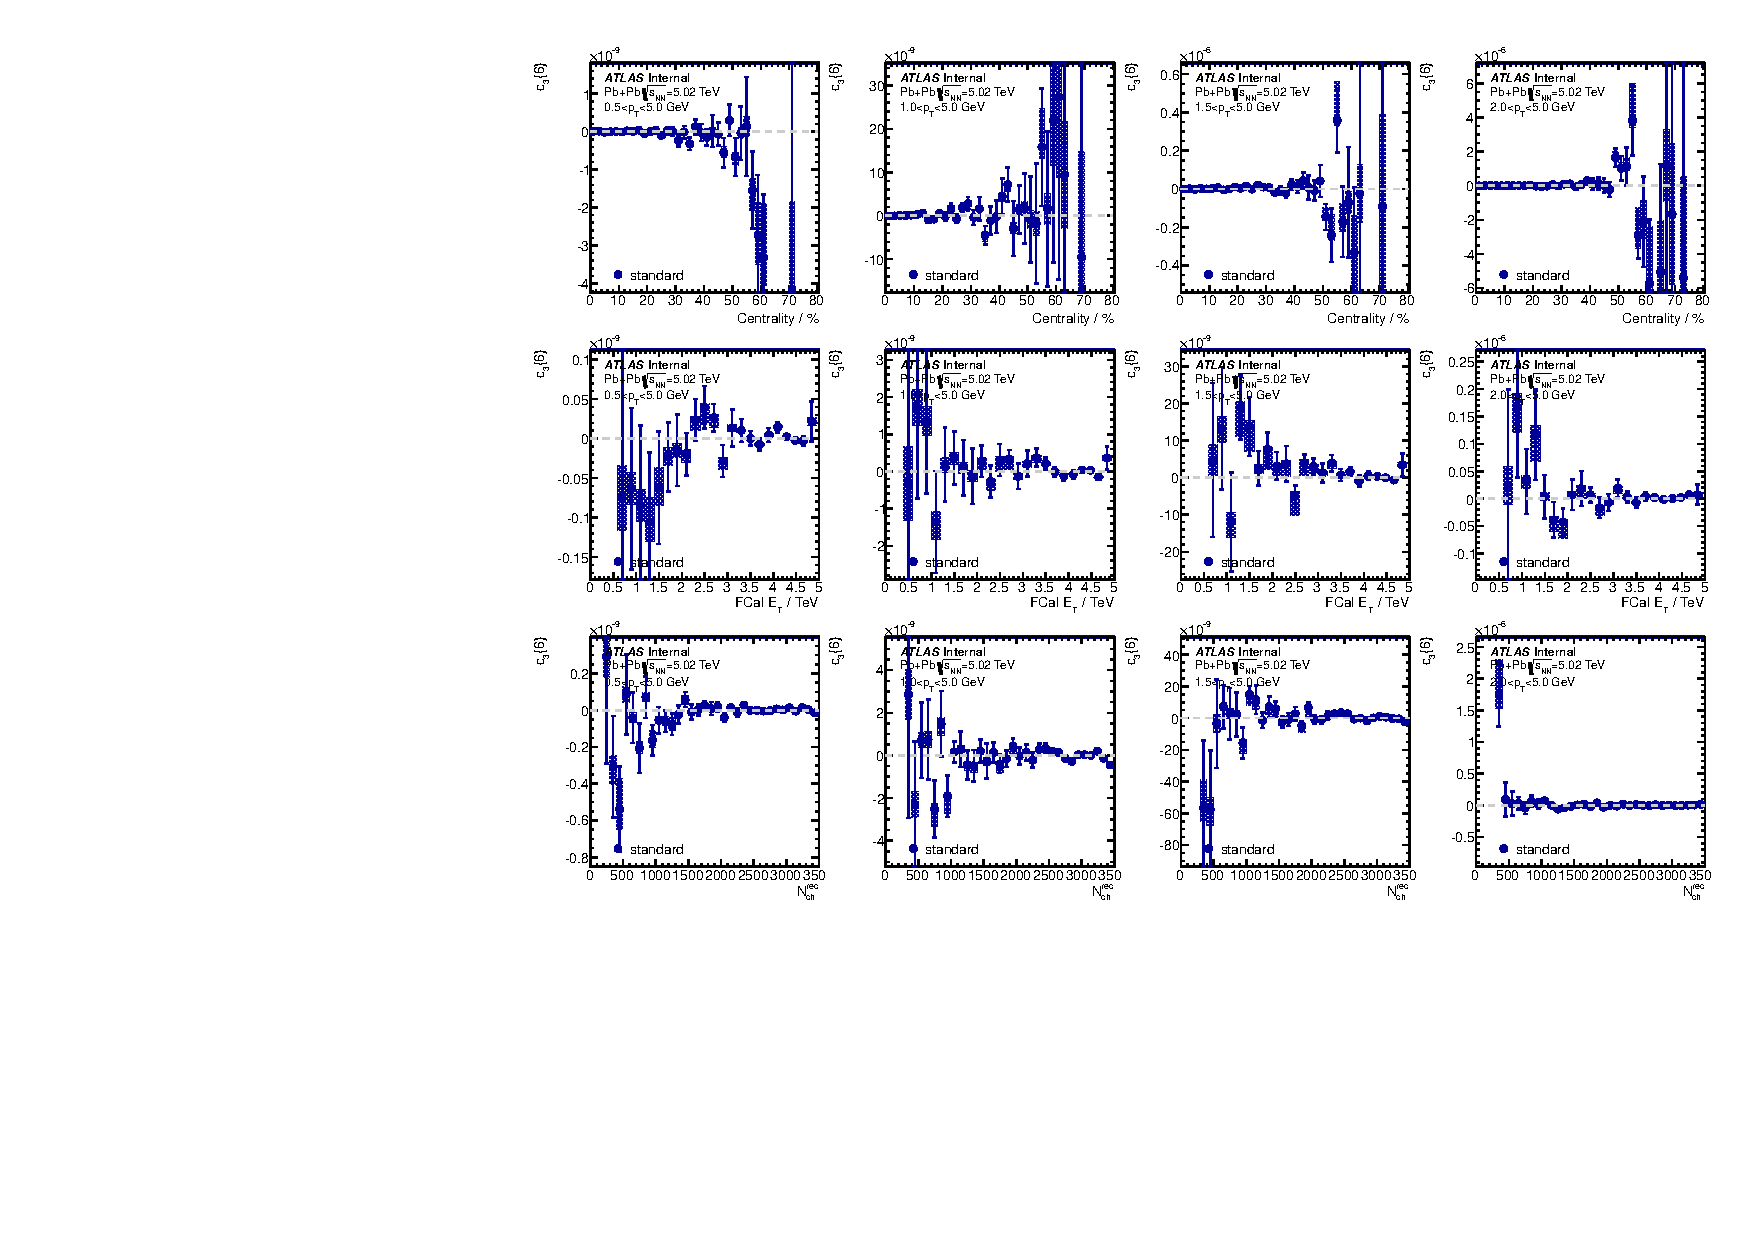
\includegraphics[width=.95\linewidth]{figs/sec_result/forQM/phy_c6_Har3.pdf}
\caption{6-particle cumulant $c_2\{6\}$ (top half) and $c_3\{6\}$ (bottom half) calculated with different $p_\text{T}$ ranges (columns) and different event class definitions (rows).}
\label{fig:result_phy_c6_Har23}
\end{figure}
Fig.~\ref{fig:result_phy_c6_Har23} shows $c_2\{6\}$ and $c_3\{6\}$ calculated with different $p_\text{T}$ ranges and different event class definitions. Unlike 4-particle cumulant, to have a well-defined $v_n\{6\}$, 6-particle cumulant needs to be larger than 0. For $v_2$, the centrality dependence of $c_2\{6\}$ follows the similar trend as $c_2\{4\}$: its magnitude reaches maximum in mid-centrality and drops to 0 in central collisions. Unlike the Gaussian fluctuation scenario, since $2k$-particle cumulant is proportional to the $2k$th power of $v_n$, this explains why the $c_2\{6\}$ with higher $p_\text{T}$ cuts yields larger magnitude. The results for the third harmonic $c_3\{6\}$ is also shown. Its magnitude is much smaller compared with $c_2\{6\}$. Unfortunately, since the magnitude of $v_3$ is significantly smaller than $v_2$, with current statistics, we could not measure significant non-zero $c_3\{6\}$: the results are consistent with within statistical uncertainties.

\begin{figure}[H]
\centering
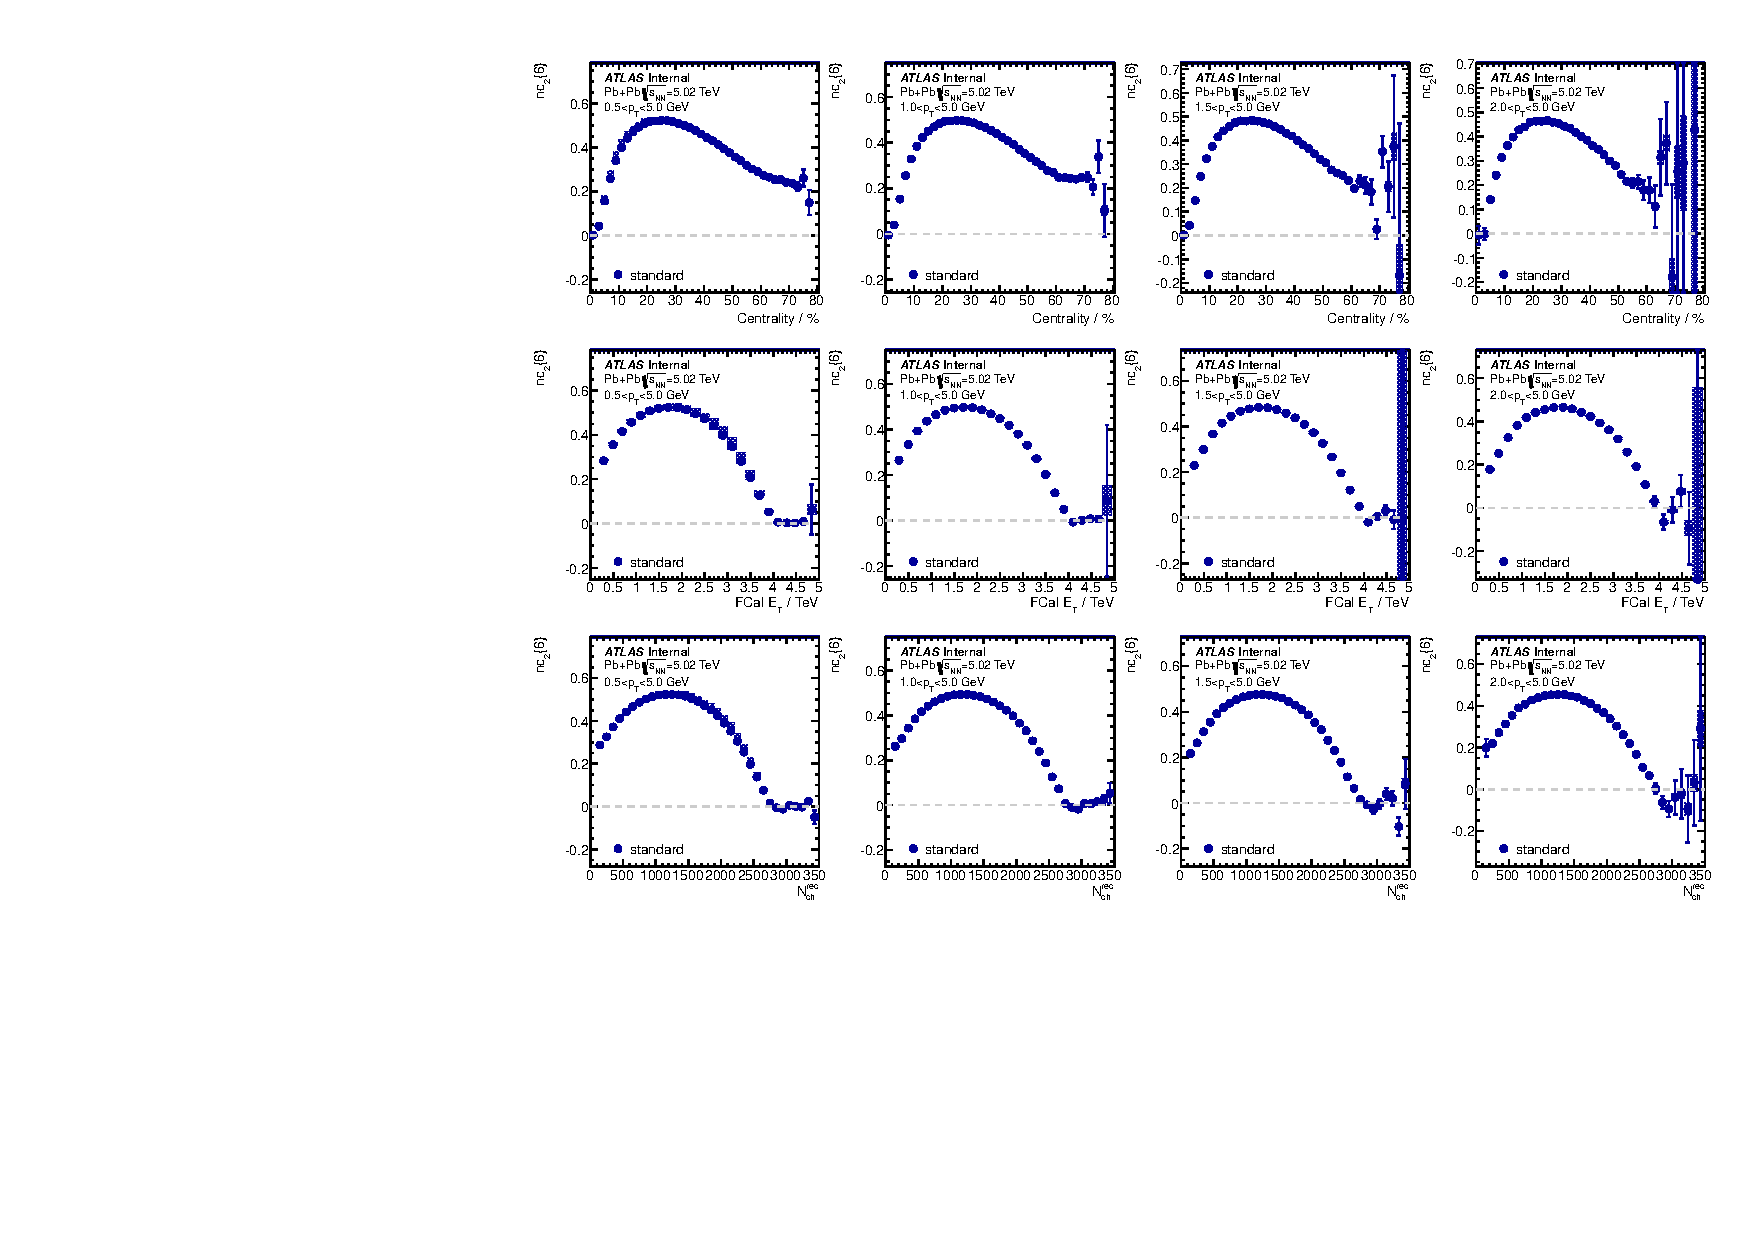
\includegraphics[width=.95\linewidth]{figs/sec_result/forQM/phy_nc6_Har2.pdf}
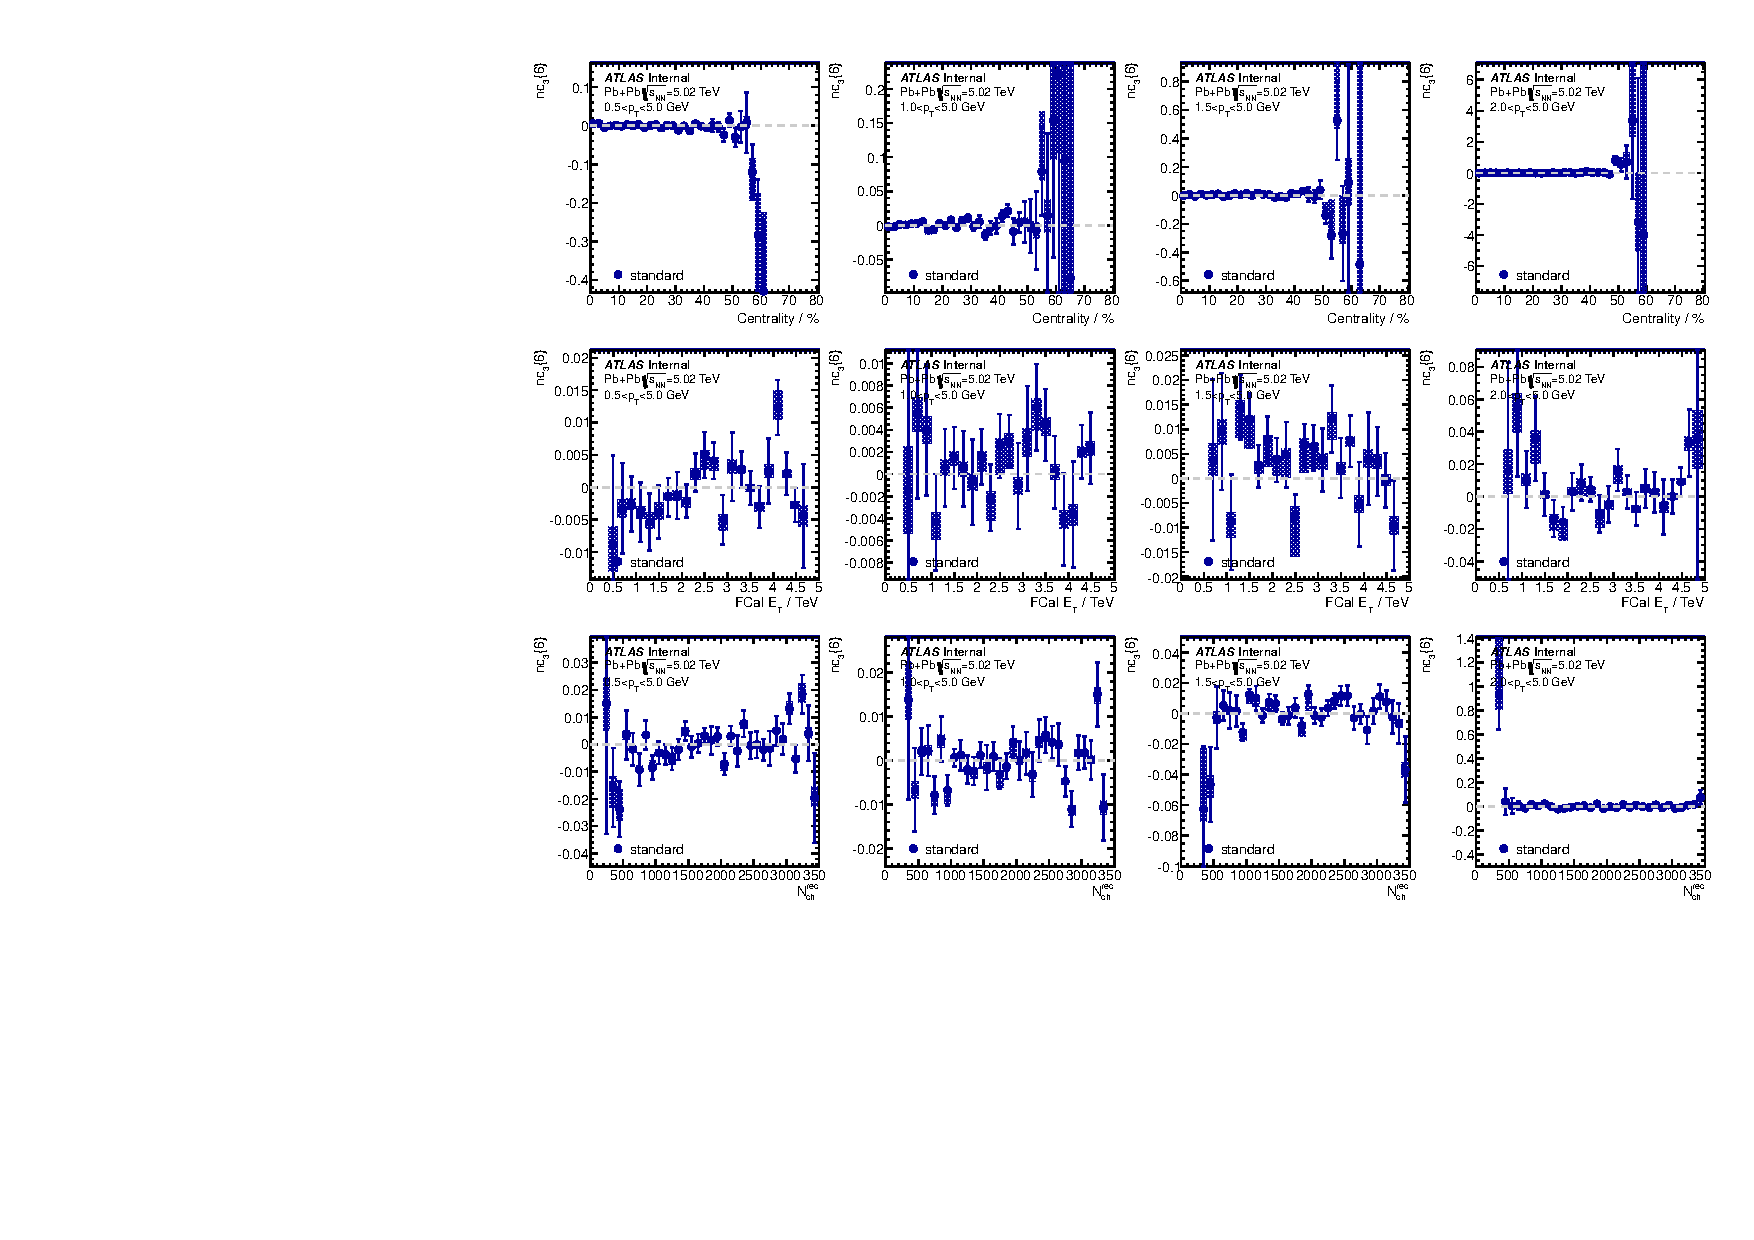
\includegraphics[width=.95\linewidth]{figs/sec_result/forQM/phy_nc6_Har3.pdf}
\caption{Normalized 6-particle cumulant $nc_2\{6\}$ (top half) and $nc_3\{6\}$ (bottom half) calculated with different $p_\text{T}$ ranges (columns) and different event class definitions (rows).}
\label{fig:result_phy_nc6_Har23}
\end{figure}
The centrality and $p_\text{T}$ dependence of 6-particle cumulant mostly originates from the centrality and $p_\text{T}$ dependence of $\bar{v}_n$. To disentangle the flow fluctuation from the mean value of flow, we have defined the normalized cumulant $nc_n\{6\}$, by dividing the 6-particle cumulant by 2-particle cumulant. The results are shown in Fig.~\ref{fig:result_phy_nc6_Har23}. For the $nc_2\{6\}$ with $1.5<p_\text{T}<5.0$ GeV, we observed a hint of double sign change in the ultra-central collisions, which is related to the single sign change of $nc_2\{4\}$. For $nc_3\{6\}$, results from all $p_\text{T}$ ranges are consistent with 0: similar conclusion as $c_3\{6\}$.

\subsection{Universality check of flow fluctuation models}
\begin{figure}[H]
\centering
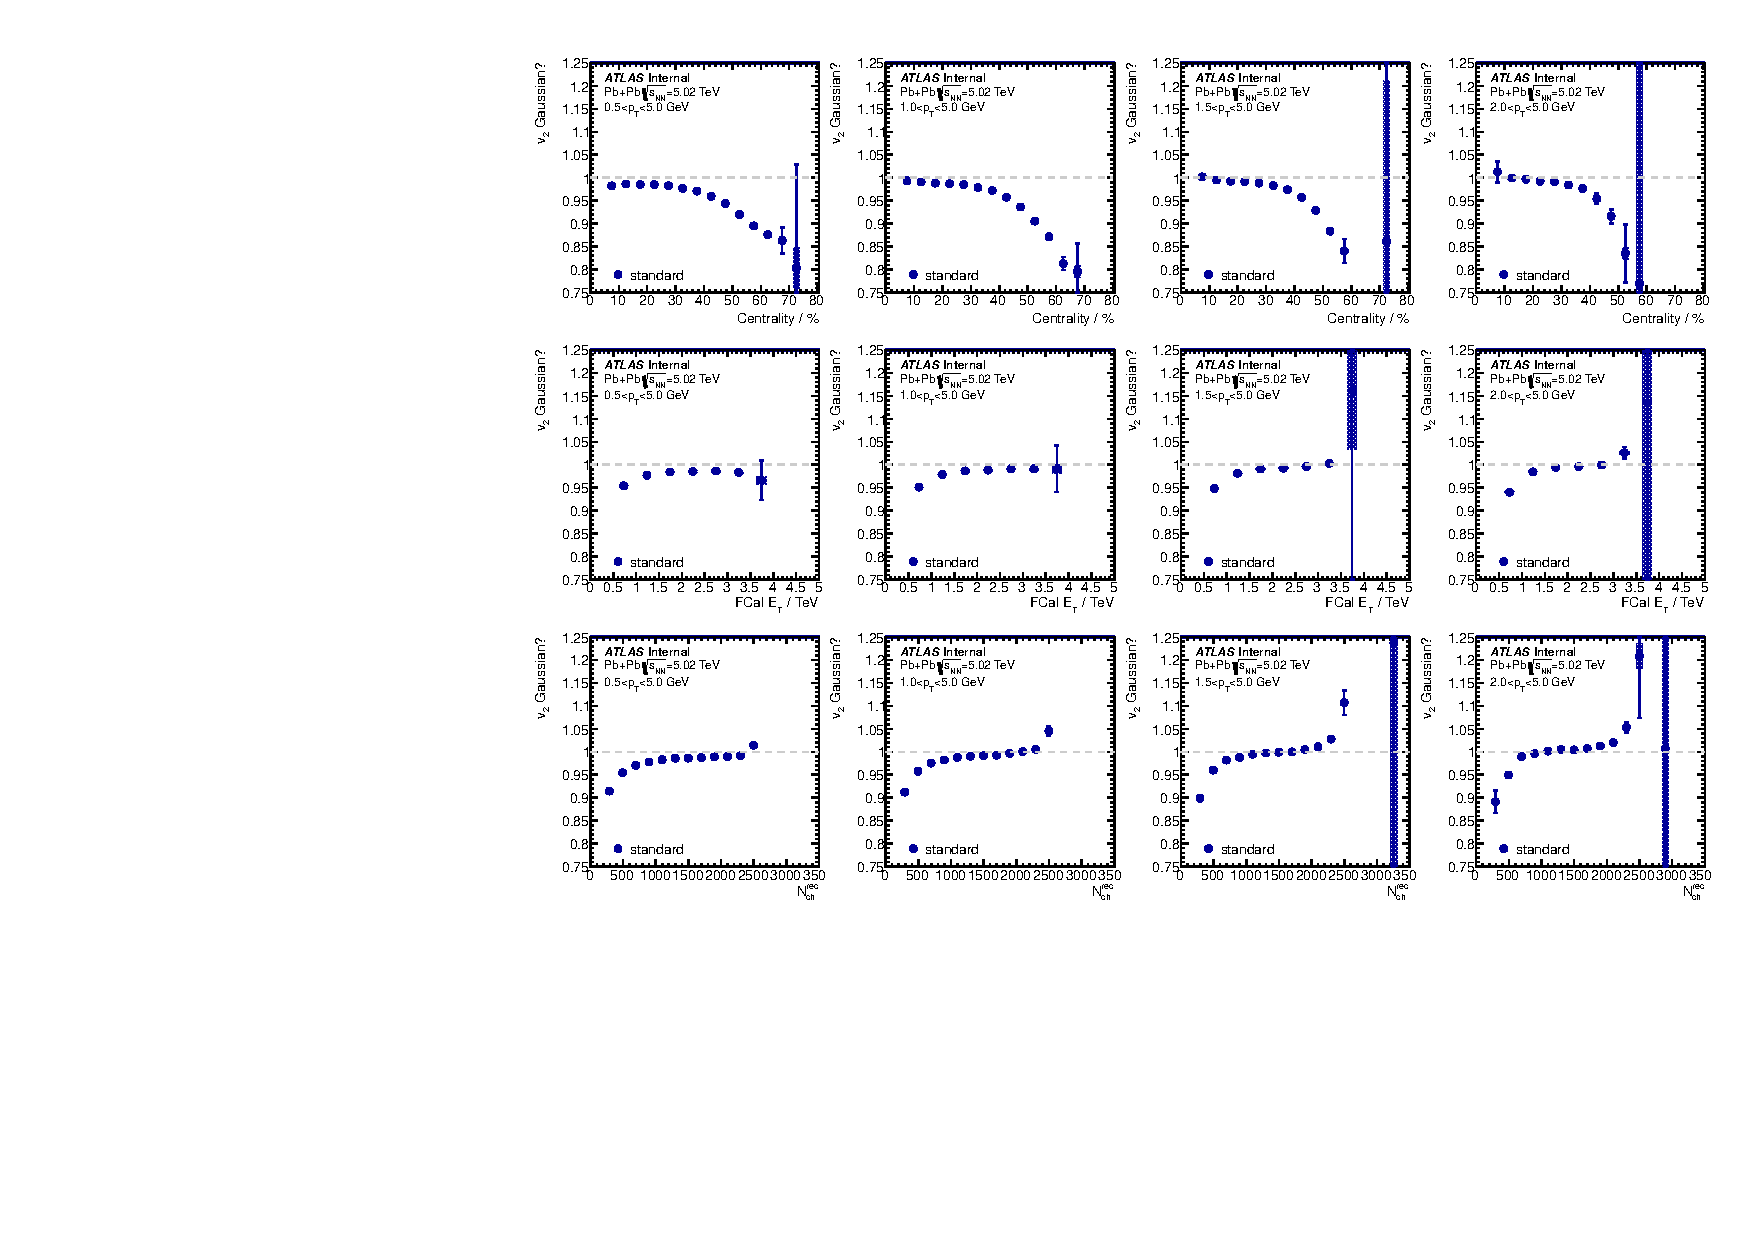
\includegraphics[width=.95\linewidth]{figs/sec_result/forQM/phy_isGauss_Har2.pdf}
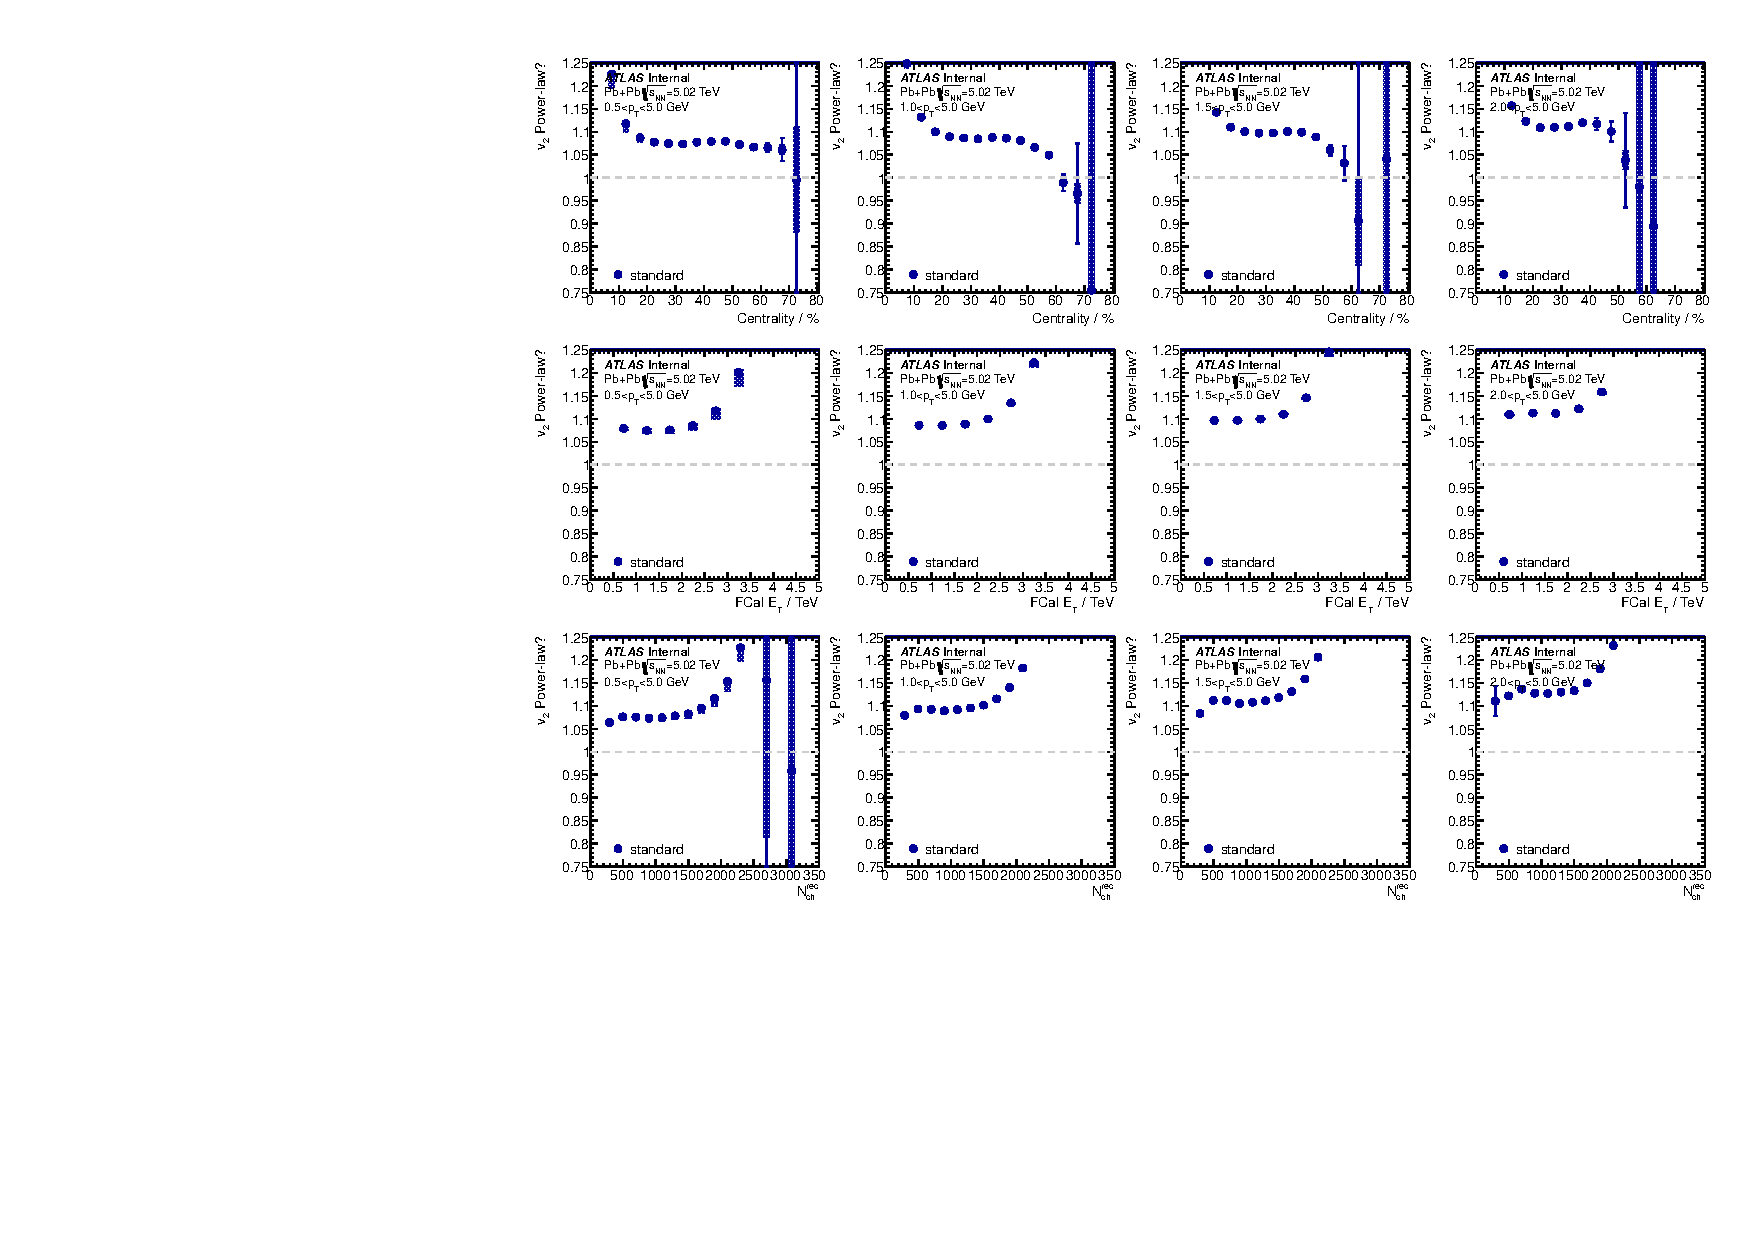
\includegraphics[width=.95\linewidth]{figs/sec_result/forQM/phy_isPower_Har2.pdf}
\caption{Check of flow fluctuation models, Gaussian (top half) or power-law (bottom half) calculated with different $p_\text{T}$ ranges (columns) and different event class definitions (rows).}
\label{fig:result_phy_fluc_Har2}
\end{figure}
To quantify the flow fluctuation in Pb+Pb, in Fig.~\ref{fig:result_phy_fluc_Har2}, we show the Gaussian universality test of $v_2$ fluctuation. As discussed in the methodology section, if the underlying flow fluctuation is Gaussian, the value should be 1. In other words, any deviation from 1 will indicate a non-Gaussian fluctuation. In Pb+Pb, the Gaussian check is consistent with 1 in central, very close to 1 in mid-central, and begins to deviate from 1 towards peripheral collisions. This trend is qualitatively consistent with the previous ATLAS $p(v_n)$ measurement, which used unfolding technique to directly measure the event-by-event $v_n$ distribution. The universality check for $v_3$ are consistent with 0, due to very large statistical uncertainties. In addition to Gaussian flow fluctuation, another competing fluctuation model follows the power-law distribution, which is shown in the same figure. Compared with the Gaussian check, the power-law check is further away from 1, meaning that the underlying flow fluctuation is closer to Gaussian than power-law. For $v_3$, there are not enough statistics to quantify whether the fluctuation follows power-law.

\subsection{Symmetric cumulant $sc_{n,m}\{4\}$ and $nsc_{n,m}\{4\}$}
\begin{figure}[H]
\centering
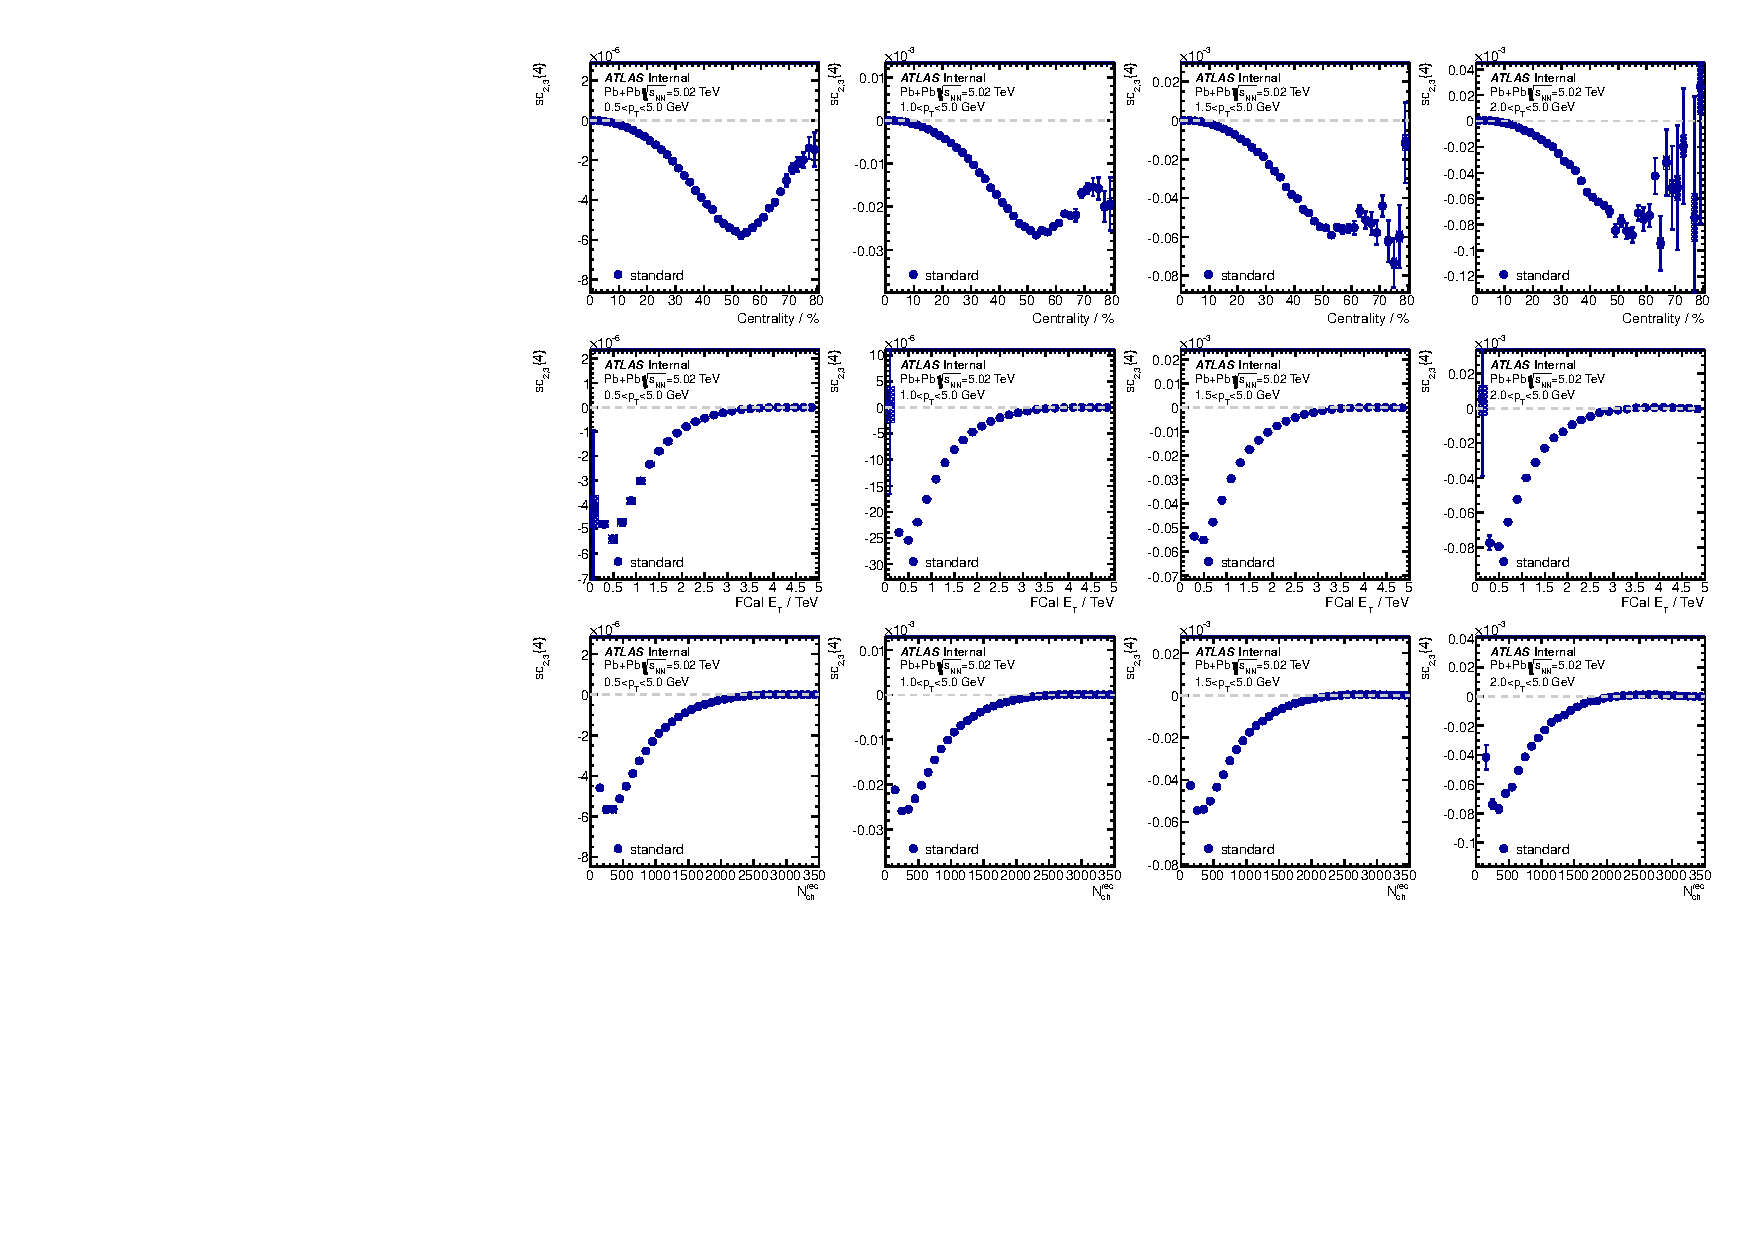
\includegraphics[width=.95\linewidth]{figs/sec_result/forQM/phy_sc_Har2.pdf}
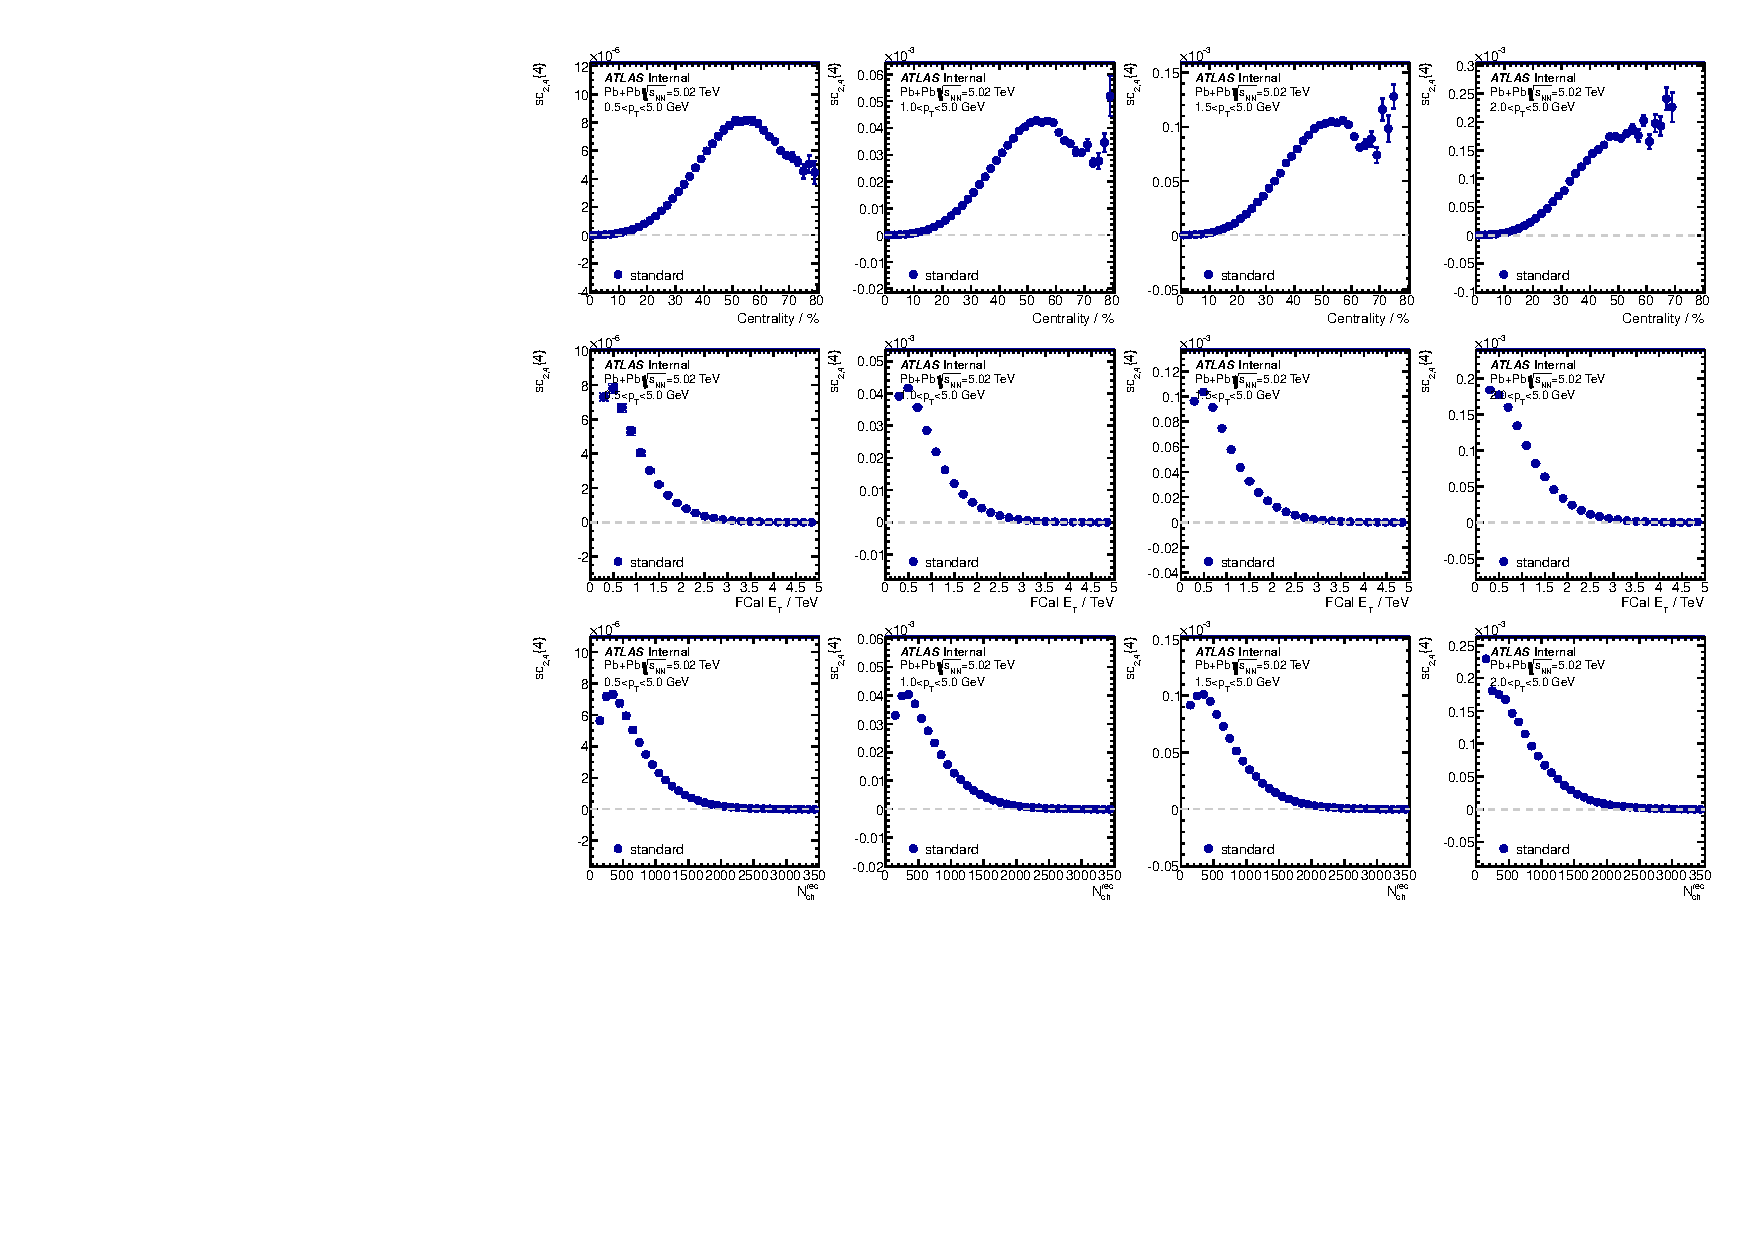
\includegraphics[width=.95\linewidth]{figs/sec_result/forQM/phy_sc_Har3.pdf}
\caption{Symmetric cumulant $sc_{2,3}\{4\}$ (top half) and $sc_{2,4}\{4\}$ (bottom half) calculated with different $p_\text{T}$ ranges (columns) and different event class definitions (rows).}
\label{fig:result_phy_sc_Har23}
\end{figure}
To unveil the correlation and fluctuation between flow harmonics $v_n$ and $v_m$, Fig.~\ref{fig:result_phy_sc_Har23} shows the symmetric cumulant $sc_{2,3}\{4\}$ and $sc_{2,4}\{4\}$ calculated with different $p_\text{T}$ ranges and different event class definitions. $sc_{2,3}\{4\}$ measures the correlation between $v_2$ and $v_3$, a negative value indicates that the correlation between $v_2$ and $v_3$ are anti-correlated. This is not hard to understand since an enhancement of elliptic flow will suppress the leading odd harmonic $v_3$. The centrality dependence of $sc_{2,3}\{4\}$ basically follows the centrality dependence of $v_2$ and $v_3$, and $sc_{2,3}\{4\}$ has a strong $p_\text{T}$ dependence, all of which will be weakened once we calculate the normalized symmetric cumulant. For $sc_{2,4}\{4\}$, the value is larger than 0, meaning that the correlation between $v_2$ and $v_4$ are positively correlated. Part of the cause is due to the similar geometric features of elliptic and quadratic flow, more importantly, the other cause is due to the non-linear component of $v_2^2$ in $v_4$, which is covered in the discussion of sign change of $c_4\{4\}$. 

\begin{figure}[H]
\centering
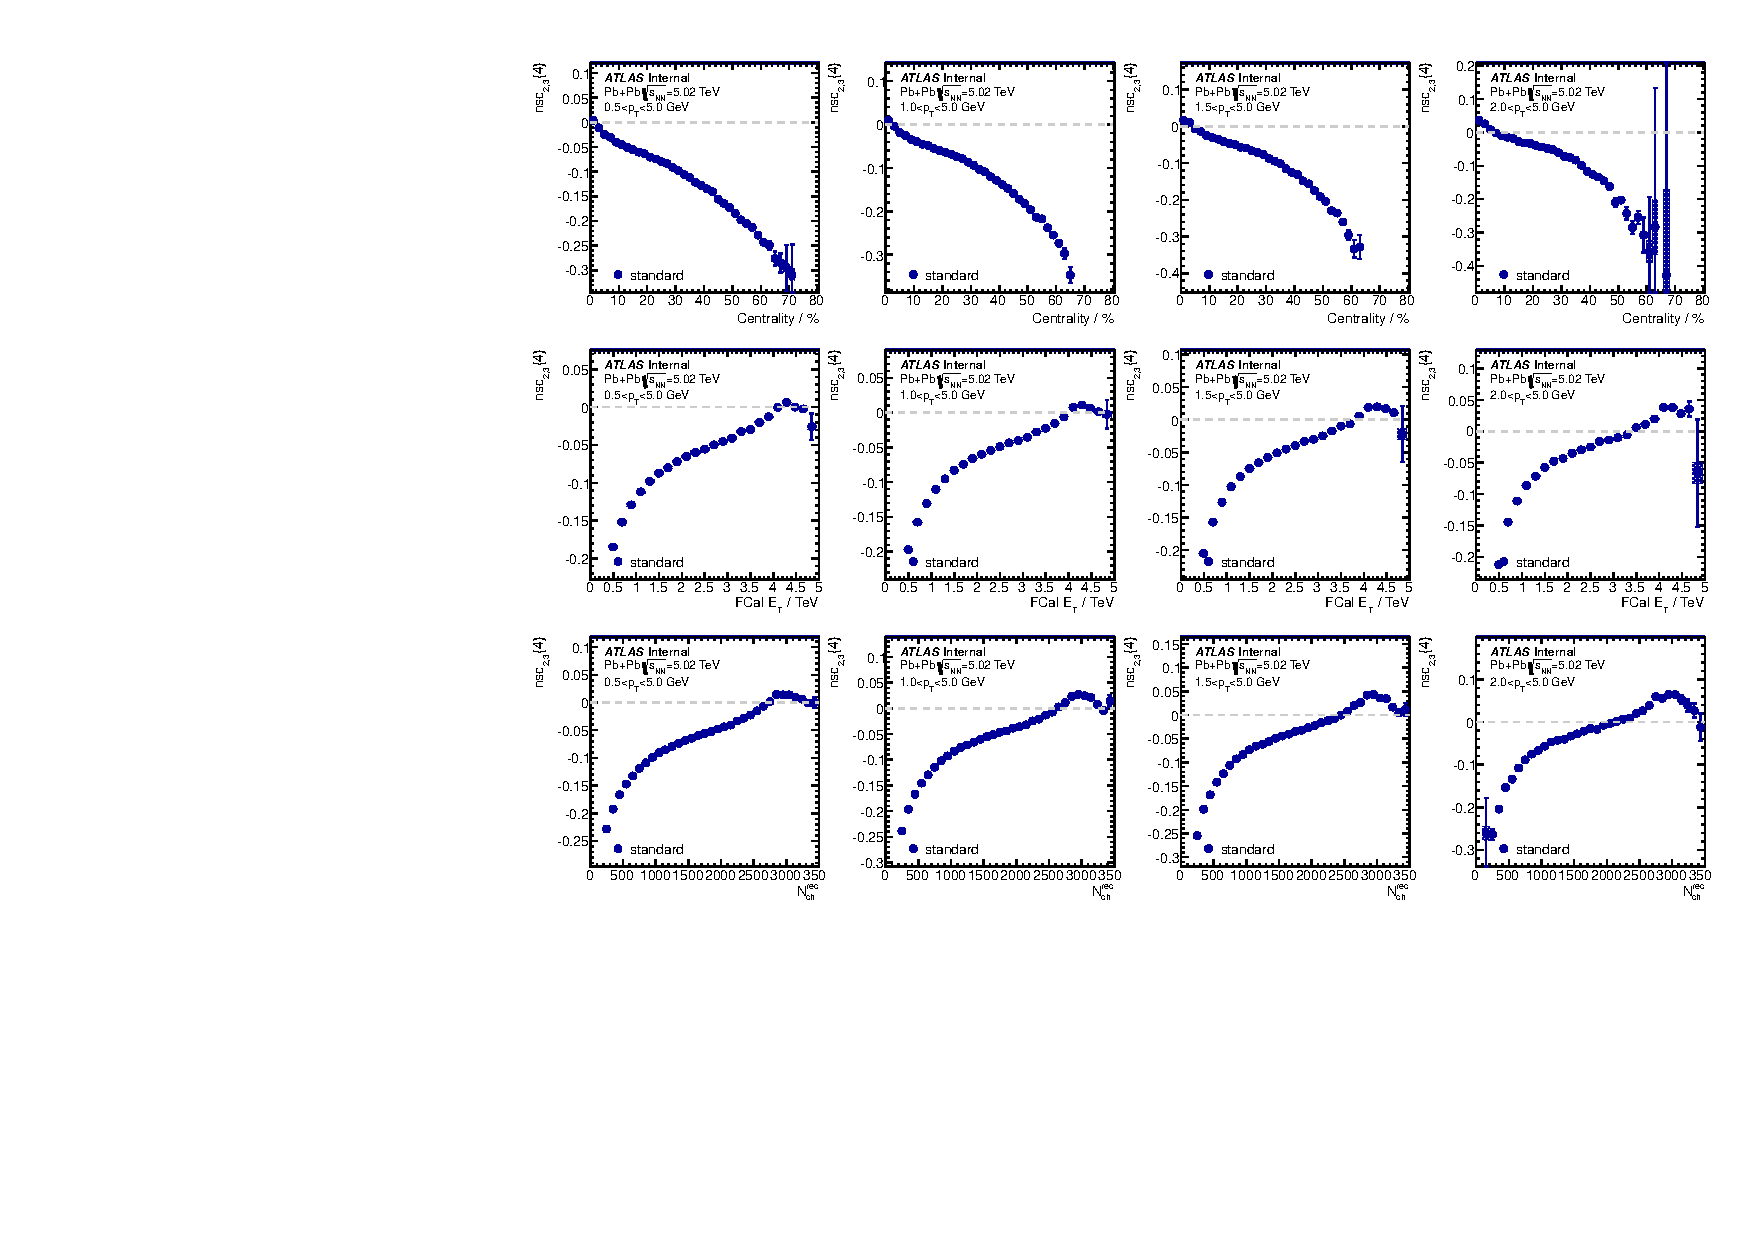
\includegraphics[width=.95\linewidth]{figs/sec_result/forQM/phy_nsc_Har2.pdf}
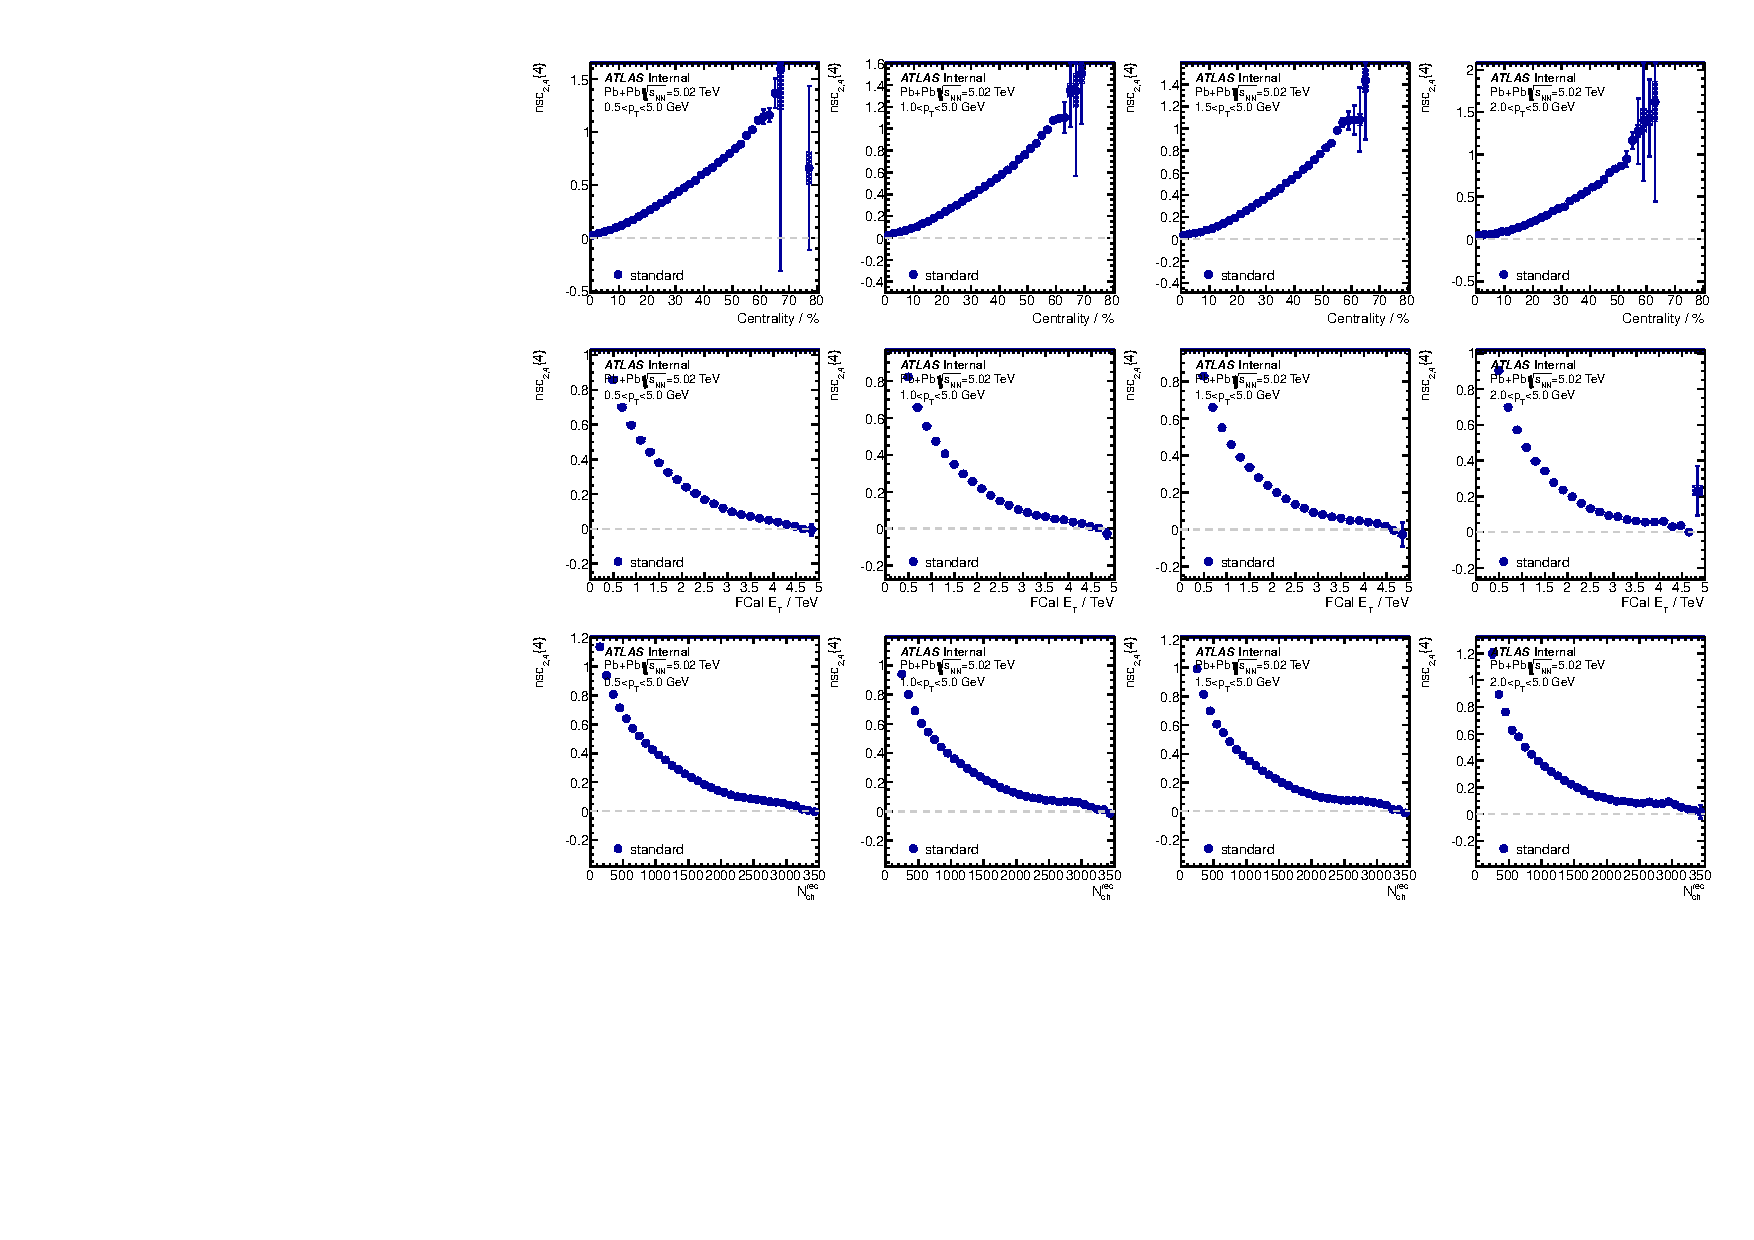
\includegraphics[width=.95\linewidth]{figs/sec_result/forQM/phy_nsc_Har3.pdf}
\caption{Normalized symmetric cumulant $nsc_{2,3}\{4\}$ (top half) and $nsc_{2,4}\{4\}$ (bottom half) calculated with different $p_\text{T}$ ranges (columns) and different event class definitions (rows).}
\label{fig:result_phy_nsc_Har23}
\end{figure}
To take out the centrality and $p_\text{T}$ dependence of symmetric cumulant, normalized symmetric cumulants $nsc_{n,m}\{4\}$ are calculated, and the results are summarized in Fig.~\ref{fig:result_phy_nsc_Har23}. For $nsc_{2,3}\{4\}$, the centrality and $p_\text{T}$ dependence are very different from $sc_{2,3}\{4\}$: the magnitude keeps increasing as collision moves towards peripheral, and the $p_\text{T}$ dependence is much weaker in the normalized case. Interestingly, similar sign change behaviour is also observed in central collision: $nsc_{2,3}\{4\}$ becomes positive for centrality $<1\%$, especially when the events are binned according to $N_{ch}^{rec}$. This sign change behavior can be explained in the similar way as the sign change of $c_2\{4\}$: centrality fluctuation changes the flow fluctuation, and results in positive correlation between $v_2$ and $v_3$. For $nsc_{2,4}\{4\}$, the centrality and $p_\text{T}$ dependence are also very different from $nsc_{2,4}\{4\}$, but no hint of sign change is observed. This could be due to the fact that $v_2\{2\}$ never drops to 0, even in central collisions, which makes $nsc_{2,4}\{4\}$ positive. However, a hint of kink is observed in ultra-central collision, indicating that the centrality fluctuation still plays a role.

\subsection{Asymmetric cumulant $ac_{n,n+m}\{3\}$ and $nac_{n,n+m}\{3\}$}
\begin{figure}[H]
\centering
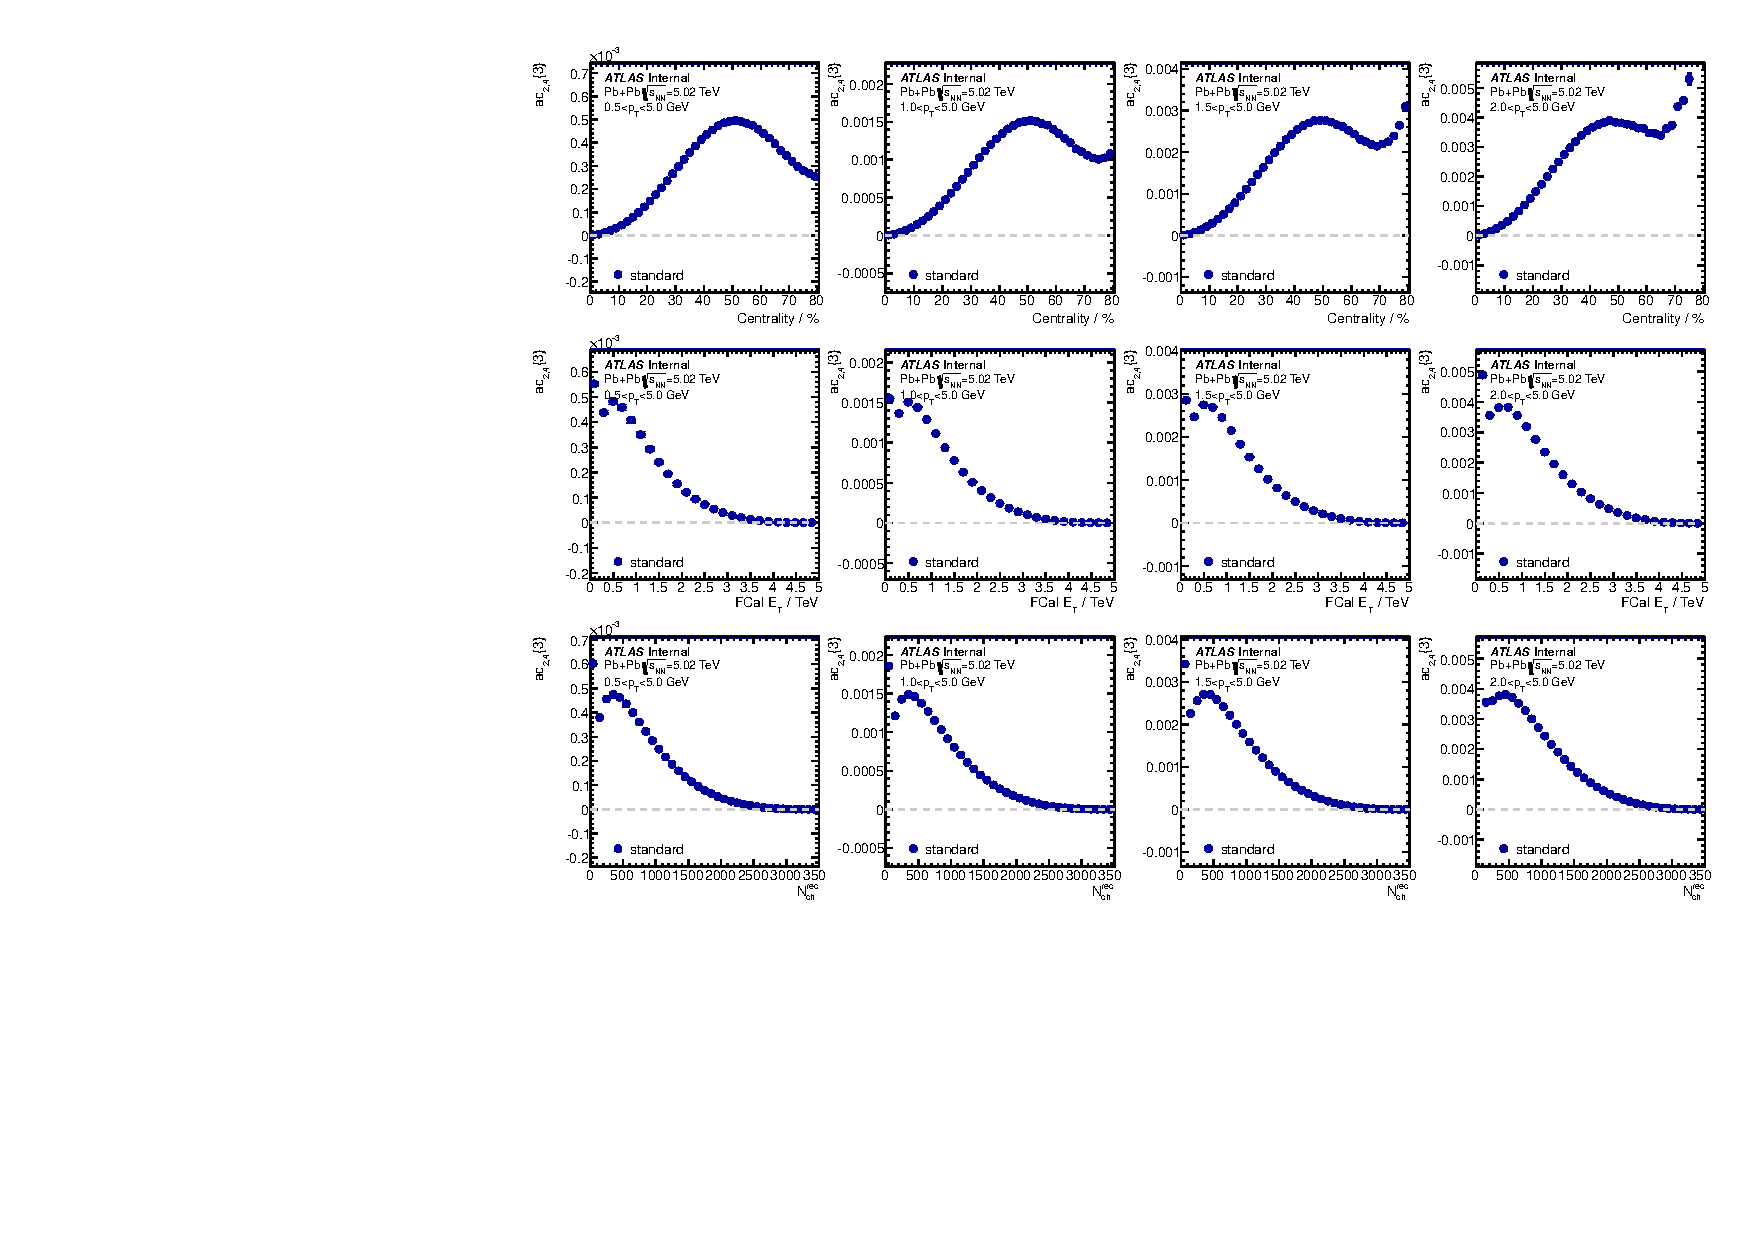
\includegraphics[width=.95\linewidth]{figs/sec_result/forQM/phy_ac_Har2.pdf}
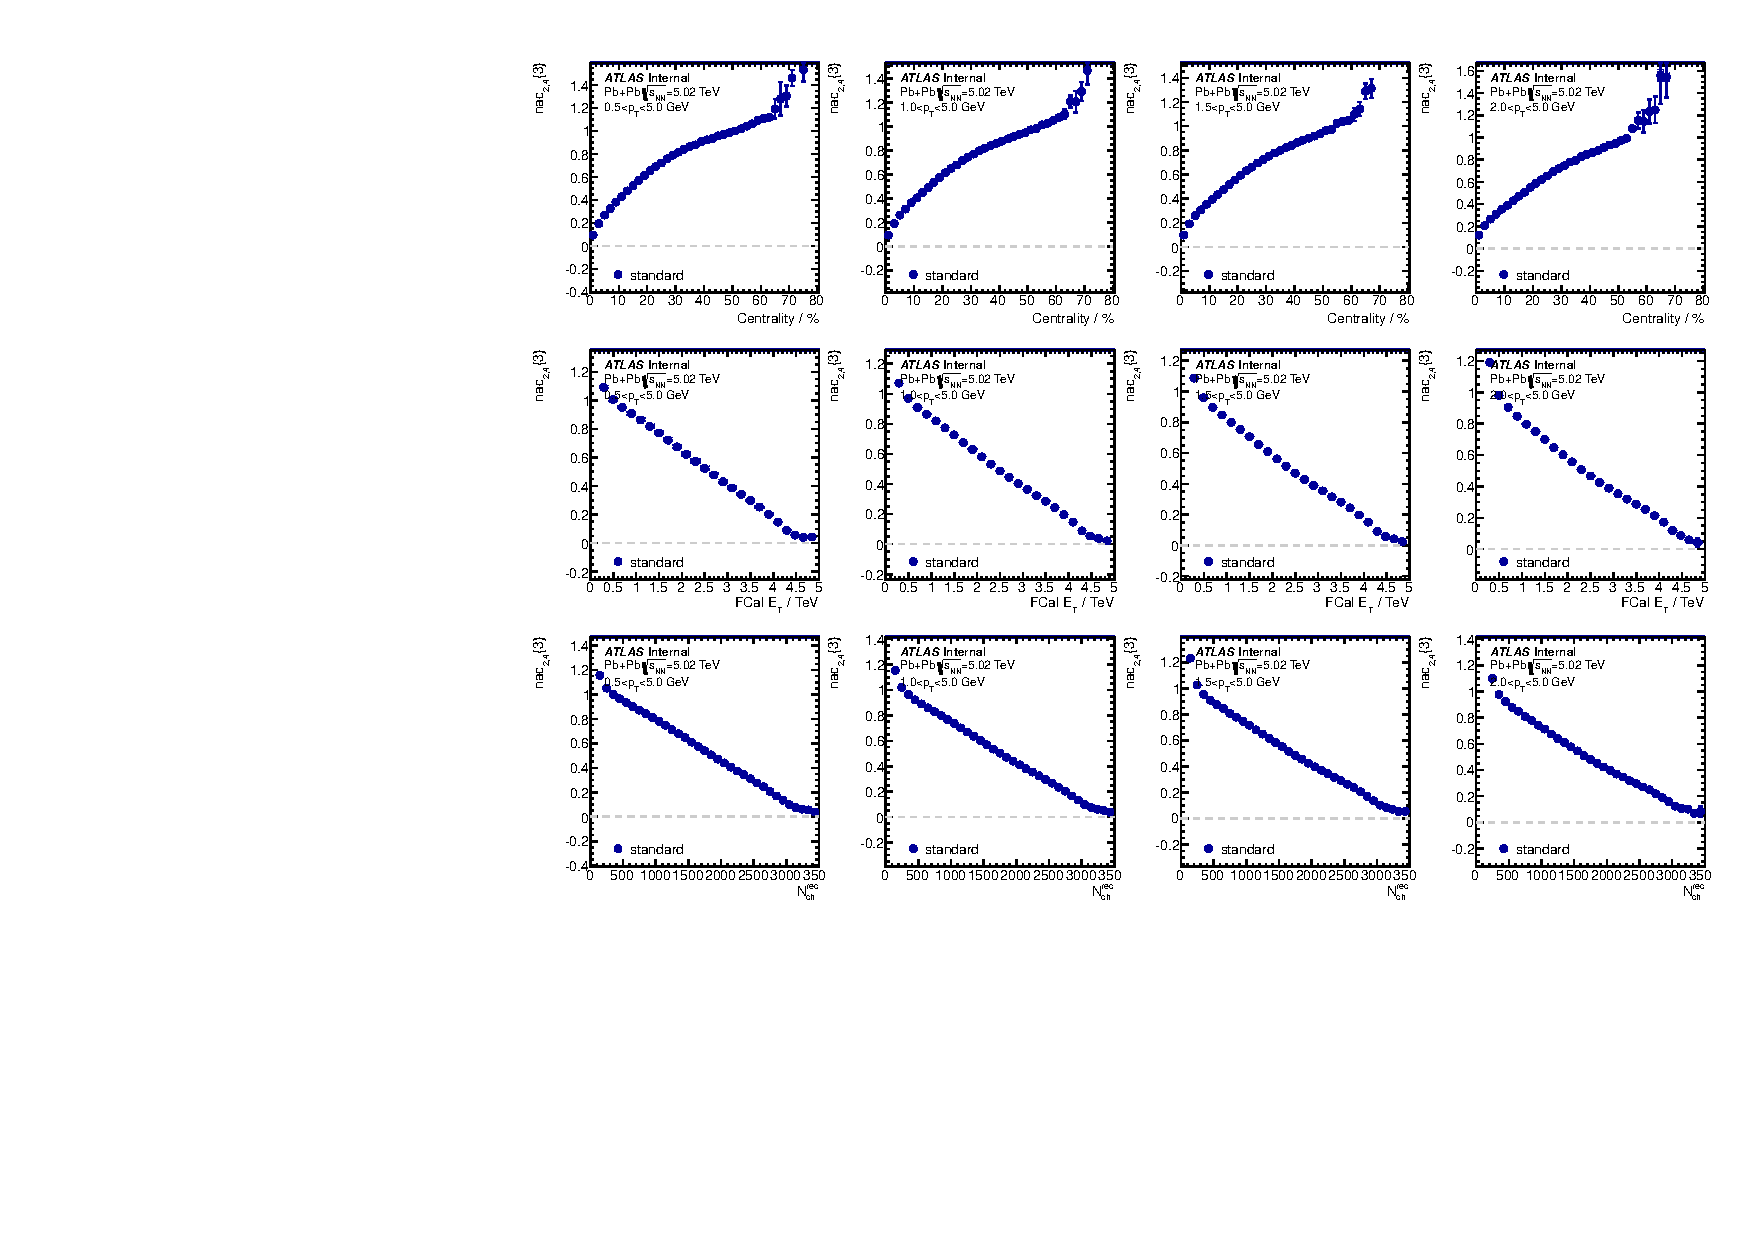
\includegraphics[width=.95\linewidth]{figs/sec_result/forQM/phy_nac_Har2.pdf}
\caption{Asymmetric cumulant $ac_{2,4}\{3\}$ (top half) and normalized asymmetric cumulant $nac_{2,4}\{3\}$ (bottom half) calculated with different $p_\text{T}$ ranges (columns) and different event class definitions (rows).}
\label{fig:result_phy_ac_Har2}
\end{figure}
In the last part of this section we show the asymmetric cumulant $ac_{2,4}\{3\}$ results in Fig.~\ref{fig:result_phy_ac_Har2}. $ac_{2,4}\{3\}$ measures the correlation among $v_2$, $v_2$ and $v_4$, which is similar to the event plane correlation that has been measured before. Like $sc_{2,4}\{4\}$, $ac_{2,4}\{3\}$ follows the similar centrality and $p_\text{T}$ dependence, most of which is due to the centrality and $p_\text{T}$ dependence of $v_2$ and $v_4$. Note that the increase of magnitude in peripheral with high $p_\text{T}$ is probably cause by the non-flow, as shown in the method comparison section. After the asymmetric cumulant is normalized, the centrality dependence becomes monotonic and the $p_\text{T}$ dependence is much weaker.









